\documentclass[a4paper,10pt]{book}
\usepackage[utf8]{inputenc}


\usepackage{amsmath}
\usepackage{amssymb}

\usepackage{cite}

\usepackage{graphicx}
\usepackage{subfig}
\usepackage{color}
\usepackage{transparent}

\usepackage{tabularx}

\usepackage{hyperref}

\newcommand{\bv}{\hbox{\boldmath $v$}}
\newcommand{\bnu}{\hbox{\boldmath $\nu$}}
\newcommand{\bomega}{\hbox{\boldmath $\omega$}}
\newcommand{\brho}{\hbox{\boldmath $\rho$}}
\newcommand{\btau}{\hbox{\boldmath $\tau$}}

\renewcommand{\bibname}{R\'ef\'erences}
\def\chaptername{Chapitre}

\begin{document}

%\include{./titlepage/titlepage}

%\pagebreak

%\include{preambule/preambule}

%\pagebreak

%% CDPR
%\chapter{Les robots parall\`eles \`a c\^ables} \label{chap0}

Il s'agit dans ce chapitre d'introduire les problématiques et méthodologies qui 
nous guideront dans notre étude de l'utilisation de l'asservissement visuel pour 
une architecture de robot très particulière, les robots parall\`eles \`a 
c\^ables. Deux objectifs animent ce travail : il s'agit dans un premier temps 
de perfectionner les fonctionnalités de saisie et manipulation d'objets de ces 
robots, et d'en améliorer les propriétés dans un second temps.

Pour cela, nous  évoquons dans une première section les avantages et 
inconvénients des structures parallèles comparativement aux structures en série. 
Les spécificités des manipulateurs à c\^ables sont introduites dans une deuxième 
section, suivie d'un rappel de leurs modèles géométriques et cinématiques. 
Nous présentons ensuite dans une troisième section la classe des manipulateurs 
de type N-1, \`a laquelle appartient le prototype sur lequel nous avons 
effectu\'e nos expérimentations et validations, et dont nous donnerons 
les principales propri\'et\'es.

%Dans une quatrième section, à la suite d'un rappel des modèles 
%d'asser\-vissement visuel, nous justifierons les choix de configuration 
%d'asservissement que nous avons opérés, et indiquerons de quelles manières 
%notre approche se démarque des travaux existants dans ce domaine précis. En 
%particulier, les robots à câbles peuvent fonctionner selon différents modes ; 
%nous montrerons comment nous avons utilisé cette spécificité pour en optimiser 
%la commande. La cinquième et dernière section présentera les problématiques de 
%l'étude de la manipulation et les choix méthodologiques qui en ont permis la 
%résolution.

\section{Manipulateurs série et parallèles} \label{chap0-0}

C'est incontestablement l'industrie qui aura été le principal vecteur de 
développe\-ment de la robotique ces deux derniers siècles. L'introduction des 
robots dans les usines s'inscrit dans une démarche d'augmentation de la 
productivité et d'amélio\-ration des performances. Cela aura permis dès lors de 
soulager le travailleur humain dans des situations de travail pénible et/ou 
répétitif, et d'augmenter ses compétences en permettant par exemple une 
précision qu'il ne saurait fournir seul, ou la possibilité de déplacer des 
charges élevées. Si la grande diversité que recouvre aujourd'hui le terme de 
{\it robot} rend extrêmement difficile l'élaboration d'une définition générique, 
nous pouvons cependant en dériver des sous-catégories plus faciles à 
appréhender. Parmi celles-ci, nous distinguons en particulier la classe des 
manipulateurs dont l'objectif sera le déplacement et positionnement d'objets 
dans l'espace.

\subsection{Définitions} \label{chap0-0-0}

Un manipulateur sera constitué de manière générale d'une base et d'un organe 
terminal, reliés par une ou plusieurs chaînes cinématiques plus ou moins 
élaborées.

Une chaîne cinématique est caractérisée par une succession de solides reliés 
par des articulations simples ou complexes. Les articulations simples peuvent 
être de nature {\it prismatique} (Fig.\ref{intro:fig0view0}) -- permettant la 
translation d'un solide par rapport à l'autre -- ou {\it rotoïdes} 
(Fig.\ref{intro:fig0view1}) -- effectuant un mouvement de rotation autour d'un 
axe donné. Des articulations complexes sont obtenues à partir de la combinaison 
de mouvements prismatiques et/ou rotoïdes : une articulation cylindrique 
(Fig.\ref{intro:fig0view2}) permet par exemple la combinaison d'un mouvement de 
translation selon un axe donné et d'un mouvement de rotation autour de ce même 
axe ; autre exemple, une articulation sphérique (Fig.\ref{intro:fig0view3}) 
combinera quant à elle trois rotations.

\begin{figure}[!ht]
  \centering
      \subfloat[Articulation simple de type prismatique]{\label{intro:fig0view0}
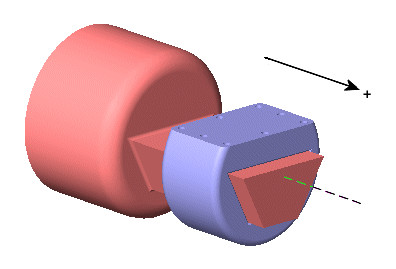
\includegraphics[width=.24\linewidth]{./chapter0/figures/prismaticJoint.jpg}} 
\hfill
    \subfloat[Articulation simple de type rotoïde]{\label{intro:fig0view1}
    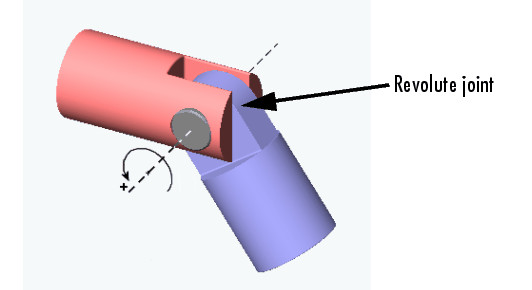
\includegraphics[width=.24\linewidth]{./chapter0/figures/revoluteJoint.jpg}} 
\hfill
  \subfloat[Articulation composée de type cylindrique]{\label{intro:fig0view2}
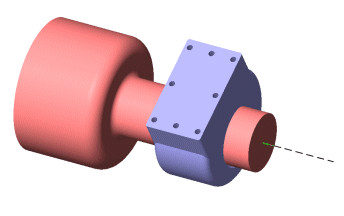
\includegraphics[width=.24\linewidth]{./chapter0/figures/cylindricalJoint.jpg}} 
\hfill
  \subfloat[Articulation composée de type sphérique]{\label{intro:fig0view3}   
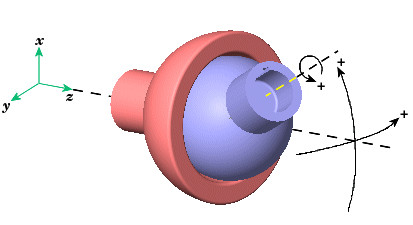
\includegraphics[width=.24\linewidth]{./chapter0/figures/sphericalJoint.jpg}}
    \caption{\footnotesize{Différents exemples d'articulations.}}
\label{intro:fig0}
\end{figure}

On appelle {\it coordonnées articulaires} l'ensemble des valeurs prises par les 
paramètres permettant de décrire l'état des articulations à un instant donné. 
Les coordonnées articulaires sont exprimées dans un espace articulaire propre à 
chaque articulation. Les paramètres nécessaires à l'expression des coordonnées 
articulaires sont généralement au nombre de 3 pour un point (ses coordonnées 
dans l'espace cartésien) et de 6 pour un solide (position cartésienne complétée 
par trois angles de rotation). Le nombre de paramètres non fixés par la 
géométrie du robot et nécessaires à la description exhaustive des coordonnées 
d'une articulation est appelé {\it degré de liberté}. Lorsque les articulations 
ne sont pas laissées libres, leur valeur dans l'{\it espace articulaire} sera 
contr\^olée par des {\it actionneurs} : on distinguera donc les {\it 
articulations actionnées} des {\it articulations passives}.

De la même manière, on parlera des {\it coordonnées opérationnelles} pour 
définir la pose de l'organe terminal, exprimées par rapport à un référentiel de 
référence. A nouveau, nous pouvons définir les degrés de liberté de l'organe 
terminal comme le nombre de paramètres contr\^olés pour le déplacer dans 
l'espace. Cette notion est à distinguer de la mobilité de l'organe terminal, 
qui 
correspond aux possibilités de déplacement de l'organe terminal, contrôlées ou 
laissées libres. Si l'on décide par exemple de contr\^oler les mouvements en 
translation, de bloquer deux rotations mais d'en laisser libre une, la mobilité 
sera de 4, mais le nombre de degrés de libertés ne sera que de 3.

Enfin, on peut définir pour chaque segment son {\it degré de connexion} comme 
étant le nombre de solides auxquels il est relié par une articulation libre ou 
actionnée. Lorsque l'ensemble des segments ont un degré de connexion égal à 2 à 
l'exception de la base et de l'organe terminal qui ont de degré de connexion 
égal à 1, on parle de {\it cha\^ine cinématique ouverte} 
(Fig.\ref{intro:fig1view0}). Lorsque l'un des segments au moins (différent de 
la 
base) possède un degré de connexion supérieur ou égal à 3, nous avons une {\it 
cha\^ine cinématique fermée} (Fig.\ref{intro:fig1view1}) 
\cite{journals/gosselin1989}. Les cha\^ines cinématiques complexes sont 
constituées de plusieurs cha\^ines fermées et/ou ouvertes.

\begin{figure}[!ht]
  \centering
      \subfloat[Schéma d'une cha\^ine cinématique 
ouverte]{\label{intro:fig1view0}
    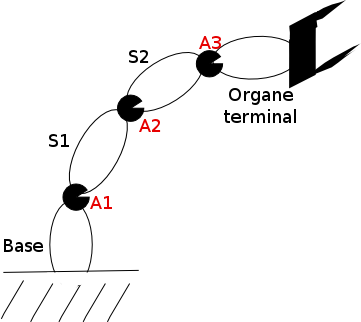
\includegraphics[width=.48\linewidth]{./chapter0/figures/openchain.png}} 
\hfill
    \subfloat[Schéma d'une cha\^ine cinématique fermée]{\label{intro:fig1view1}
    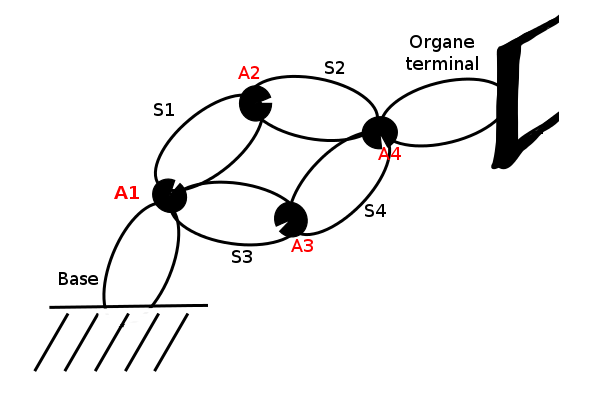
\includegraphics[width=.48\linewidth]{./chapter0/figures/closedchain.png}}
    \caption{\footnotesize{Exemples de cha\^ines cinématiques ouvertes et 
fermées : les $S_i$ représentent les différents segments intermédiaires, tandis 
que les $A_i$ correspondent aux articulations. Dans Fig.\ref{intro:fig1view0}, 
tous les segments $S_i$ ont un degré de connexion égal à 2 ; seuls la base et 
l'organe terminal ont un degré de connexion égal à 1. On peut voir au 
contraire dans Fig.\ref{intro:fig1view1} que tous les segments $S_i$ -- \`a 
l'exception donc de la base et de l'organe terminal -- possèdent un degré de 
connexion \'egal à 3.}}
\label{intro:fig1}
\end{figure}

\subsection{Architectures séries} \label{chap0-0-1}

{\it On appelle robot série un système constitué d'une chaîne cinématique 
ouverte dont chaque segment est relié au suivant par une articulation simple} 
(Fig.\ref{intro:fig2}). Longtemps dominants dans l'industrie, les robots séries 
ont été privilégiés grâce à un erelative simplicité de la commande et un espace 
de travail important.

\begin{figure}[!ht]
  \centering
      \subfloat[Robot série présentant 3 articulations 
rotoïdes]{\label{intro:fig2view0}
    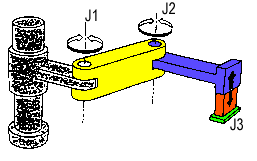
\includegraphics[width=.48\linewidth]{./chapter0/figures/serialrobot01.png}} 
\hfill
    \subfloat[Robot série présentant 3 articulations 
prismatiques]{\label{intro:fig2view1}
    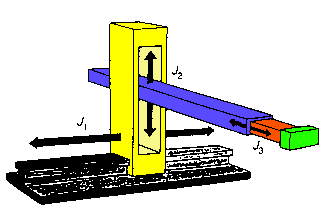
\includegraphics[width=.48\linewidth]{./chapter0/figures/serialrobot02.png}}
    \caption{\footnotesize{Exemples de robots séries (type SCARA et 
cart\'esien)}}
\label{intro:fig2}
\end{figure}

Une architecture série présente toutefois plusieurs inconvénients non 
négli\-gea\-bles dans un contexte industriel tels que :
\begin{itemize}
 \item chaque segment et articulation porte la charge de tous ceux qui leur 
succèdent dans la chaîne cinématique, ce qui pénalise la dynamique : segments 
et 
articulations doivent donc être rigidifiés et deviennent plus lourds, 
 \item les erreurs de positionnement se propagent de segments en segments ; la 
précision tout comme la répétabilité du manipulateur en sont affectées,
 \item les charges manipulables ne peuvent être \'elev\'ees, en raison des 
sollicitations en flexion sur les segments et de l'effet de bras de levier sur 
les premiers segments.
\end{itemize}

Ainsi, une architecture série impose souvent un dispositif imposant, dont la 
précision, la dynamique et la faible capacité de charges se révèleront 
insuffisants pour certaines tâches requises en particulier par l'industrie 
moderne.

Constitu\'ees de plusieurs cha\^ines cin\'ematiques ferm\'ees, les 
architectures parallèles pr\'sentent une alternative efficace aux limites des 
robots s\'eries.  Leurs caractéristiques, sur lesquel\-les nous allons \`a 
pr\'esent nous pencher, ont contribué à ce qu'elles s'installent 
progressivement 
dans le paysage de la robotique.

\subsection{Architectures parallèles} \label{chap0-0-2}

Une définition des robots parallèles est donnée dans \cite{merlet1997robots} :\\
{\it Un manipulateur parallèle est constitué d’un organe terminal à $n$ degrés 
de li\-berté et d’une base fixe, reliés entre eux par au moins deux chaînes
cinématiques indépendantes, la motorisation s’effectuant par $n$ actionneurs 
simples.}\\

Parmi les exemples les plus cités dans la littérature, nous trouvons 
la plate-forme de Gough-Stewart \cite{1956:Gough}, \cite{1965:Stewart} 
(Fig.\ref{intro:fig3view0},\ref{intro:fig3view1})et le 
robot Delta \cite{1988:Clavel} (Fig.\ref{intro:fig3view2}).

Initialement développée pour des applications li\'ees \`a l'industrie 
automobile (Fig.\ref{intro:fig3view0}), la plate-forme de Gough-Stewart a par 
la 
suite été utilisée dans des applications diverses parmi lesquelles les 
simulateurs de vols (Fig.\ref{intro:fig3view1}). Sa plate-forme mobile peut 
être déplacée selon 6 degrés de liberté (3 translations $+$ 3 rotations) à 
l'aide de six jambes indépendantes actionnées par des vérins pneumatiques. Les 
articulations la reliant à la base (cardan) et à la plate-forme (rotule) sont 
quant à elles laissées libres.

Le robot Delta (Fig.\ref{intro:fig3view2}) permet un déplacement de sa 
platforme 
selon les trois degrés de liberté de translation. Trois jambes sont utilisées 
pour cela, chacune étant reliée à la base par une articulation rotoïde à un 
levier, lui-même relié à un parallélogramme par une seconde articulation 
rotoïde, une troisième articulation rotoïde liant ce segment à l'organe 
terminal. Il peut atteindre des vitesses allant jusqu'à 10 m/s et des 
accélérations jusqu'à 20G, ce qui le rend particulièrement adapté pour des 
tâches de conditionnement. 

\begin{figure}[!ht]
  \centering
      \subfloat[Plateforme de Gough utilisée dans une usine de 
pneumatiques]{\label{intro:fig3view0}
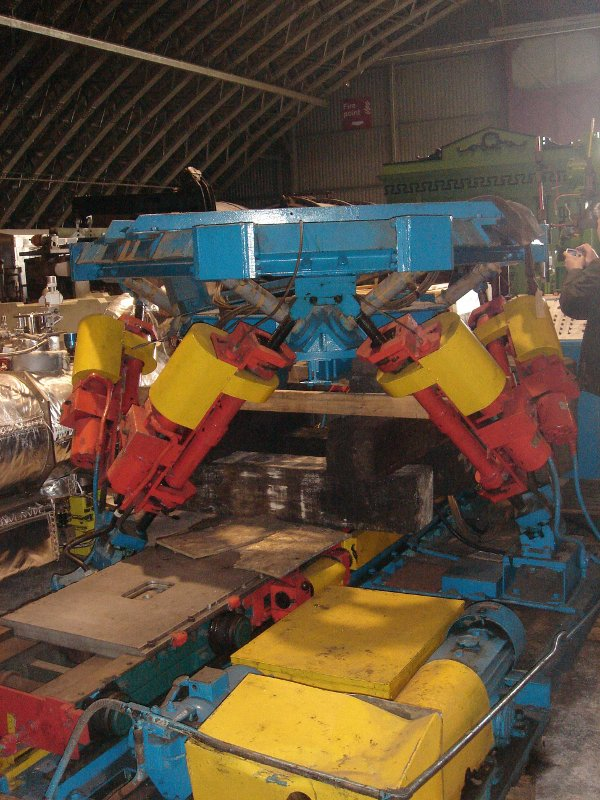
\includegraphics[width=.34\linewidth]{./chapter0/figures/parallelrobot01.jpg}} 
\hfill
    \subfloat[Plateforme de Gough-Stewart utilisée pour des simulateurs de 
vols]{\label{intro:fig3view1} 
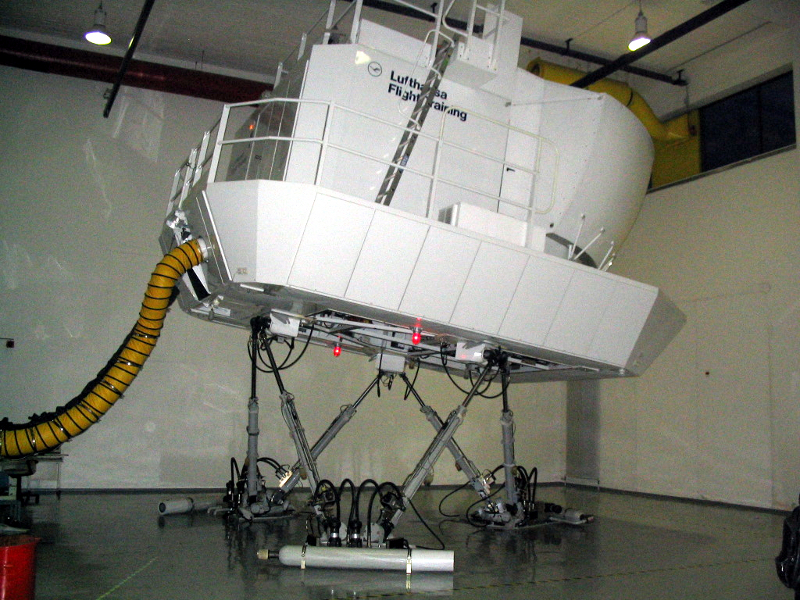
\includegraphics[width=.60\linewidth]{./chapter0/figures/parallelrobot02.jpg}} 
\\
    \subfloat[Robot Delta, particulièrement adapté aux tâches de 
conditionnement 
ou de ``pick and place'']{\label{intro:fig3view2}  
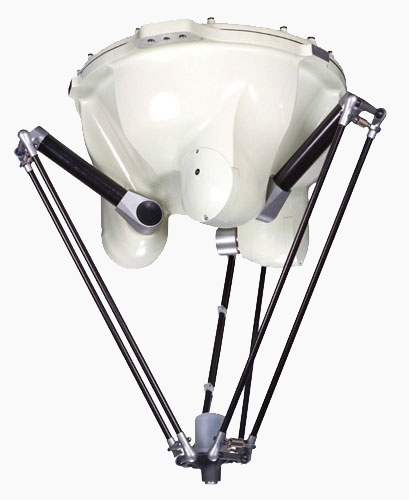
\includegraphics[width=.45\linewidth]{./chapter0/figures/parallelrobot03.jpg}}
    \caption{\footnotesize{Exemples de robots parallèles}}
\label{intro:fig3}
\end{figure}

De manière générale, les manipulateurs parallèles présentent les 
caractéristi\-ques sui\-vantes permettant de les comparer avantageusement aux 
manipulateurs séries :
\begin{itemize}
 \item une précision accrue par un mécanisme de {\bf compensation} des erreurs 
entre les différentes chaînes cinématiques (parfois appelées {\it jambes}),
 \item une capacité de charge élevée due à la {\bf répartition} de la charge 
sur 
les différentes jambes,
 \item une rigidité élevée car les éléments de chaînes sont sollicités en 
traction/compression plutôt qu'en flexion.
 \item une dynamique élevée conséquente de la {\bf coopération} des différentes 
jam\-bes dans le positionnement de l'organe terminal.
\end{itemize}

Toutefois, les mécanismes parallèles possèdent plusieurs inconvénients qui 
doivent être pris en compte lors du choix d'une architecture :
\begin{itemize}
 \item des relations complexes entre entrées et sorties,
 \item des positions dites {\it singulières} pouvant conduire à une perte de 
contrôle du manipulateur, et qui limite l'espace de travail.
 \item un espace de travail restreint par les limites de variation des 
variables articulaires. A titre d'exemple, la variation d'altitude d'une 
plate-forme de Gough-Stewart ne peut excéder la course des actionneurs 
linéaires des jambes.
\end{itemize}

L'architecture des robots parallèles à c\^ables que nous allons présenter dans 
la section suivante a été proposée dans le but de s'affranchir de la contrainte 
de limitation de l'espace de travail, qui est une contrainte forte des 
mécanismes parallèles \cite{journals/jfr/AlbusBD93}, 
\cite{1985:Landsberger.Sheridan*1}. L'intégralité des travaux présentés 
dans ce manuscrit étant consacré à l'étude et au développement de cette 
catégorie particulière de manipulateurs, nous utiliserons dorénavant pour les 
désigner les noms de robots, manipulateurs, robots parallèles à câbles ou CDPR 
(pour {\it cable-driven parallel robot}).

\section{Les manipulateurs parallèles à câbles} \label{chap0-1}

Les manipulateurs parallèles à câbles présentent une structure en chaînes 
cinéma\-tiques fermées, la base et la plate-forme étant reliées au moyen de 
câbles. Les actionneurs sont en général positionnés sur la base et leur 
fonction 
consiste à contrôler la longueur des câbles.

Afin de contrôler la longueur des câbles, plusieurs types de systèmes peuvent 
être utilisés, parmi lesquels :
\begin{itemize}
 \item un tambour actionné par un moteur rotatif sur lequel s'enroule ou se 
déroule le câble (Fig.\ref{intro:fig4view0}). La mesure de la longueur du câble 
déroulé est obtenue en mesurant la rotation du tambour ; cette mesure est 
relativement imprécise si l'enroulement n'est pas guidé.
 \item le câble est attaché au chariot d'un actionneur linéaire, un système de 
démultiplication à poulies permettant d'amplifier le déplacement du câble 
(Fig.\ref{intro:fig4view1}). La mesure du déplacement du chariot permet une 
estimation précise de la longueur du câble \cite{merlet2008}. 
\end{itemize}

\begin{figure}[!ht]
  \centering
      \subfloat[L'enroulement et le déroulement des câble se fait ici par un 
système de poulie actionnée par un moteur]{\label{intro:fig4view0}   
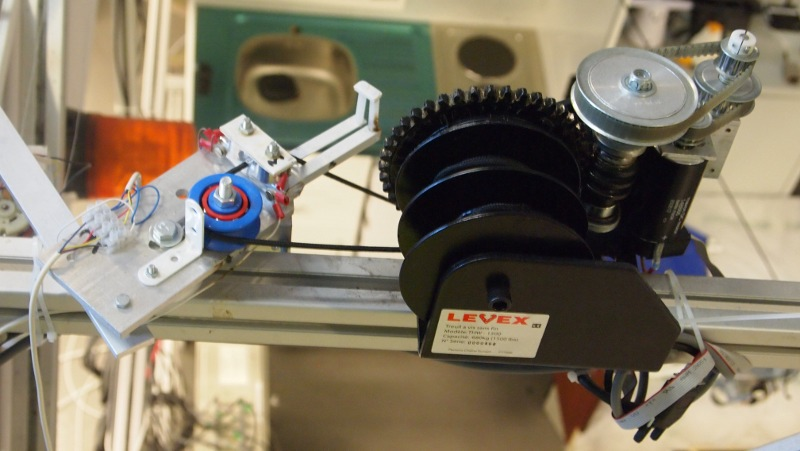
\includegraphics[width=.55\linewidth]{./chapter0/figures/winchesactuator.jpg}} 
\hfill
    \subfloat[Les câbles sont fixés à des plate-formes pouvant se déplacer 
linéairement sur des rails, permettant un contrôle de la 
longueur]{\label{intro:fig4view1}   
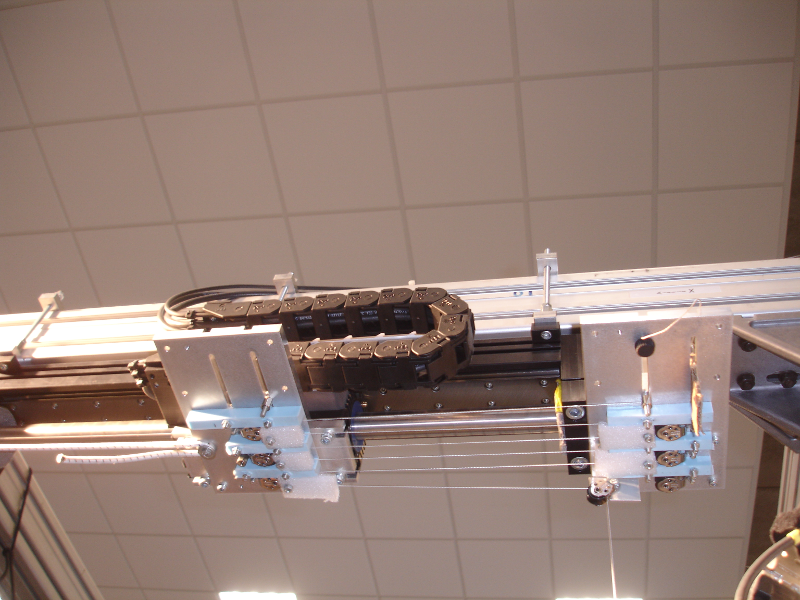
\includegraphics[width=.42\linewidth]{./chapter0/figures/linearactuator.png}}
    \caption{\footnotesize Deux types d'articulations et d'actionnement pour un 
robot à câble}
\label{intro:fig4}
\end{figure}

Dans tous les cas, ces systèmes permettent d'obtenir une très large variation 
sur les longueurs des câbles, solutionnant ainsi le problème de l'espace de 
travail. On a pu ainsi construire des robots travaillant sur des volumes de
$100m\times35m\times35m$ ({\tt Marionet-Crane}, \cite{merlet2010} 
Fig.\ref{intro:fig7view0}).

Toutefois, quelque-soit le type d'articulation et d'actionnement choisis, la 
force que peut exercer un seul câble sur l'organe terminal est nécessairement 
unilatérale : {\em un câble seul peut tirer, mais ne peut pas pousser la 
plate-forme}. Il faut donc, pour pouvoir contrôler le mouvement dans son 
intégralité, que les câbles subissent une opposition. Il a ainsi été montré que 
$n+1$ câbles au minimum sont requis pour assurer le contrôle de $n$ degrés de 
liberté \cite{1994:Ming.Higuchi}. On peut cependant considérer la gravité comme 
une force unilatérale et la représenter comme un câble virtuel jouant le rôle 
d'opposition : il est ainsi possible de n'utiliser que $n$ câbles pour $n$ 
degrés de liberté.

On distingue donc deux types de configurations pour un robot parallèle à câbles 
:
\begin{itemize}
 \item en {\it configuration suspendue} (Fig.\ref{intro:fig5view1}), la gravité 
agit comme un câble virtuel : les câbles sont fixés généralement au point le 
plus haut du dispositif, et $n$ suffisent pour déplacer et orienter l'organe 
terminal selon $n$ degrés de liberté. On retrouve parfois ce type de 
configuration dans la littérature sous le nom de {\it grue}/{\it crane}. A 
titre d'exemple, le manipulateur {\it Nist Spider} 
\cite{1992:Albus.Bostelman.ea} présente une configuration suspendue.
 \item en {\it configuration pleinement contrainte} 
(Fig.\ref{intro:fig5view0}), 
les câbles travaillent en opposition et $n+1$ sont nécessaires pour assurer des 
déplacements et l'application de forces correspondant à $n$ degrés de liberté.
\end{itemize}

\begin{figure}[!ht]
  \centering
     \subfloat[Exemple de configuration pleinement 
contrainte]{\label{intro:fig5view0}

\includegraphics[width=.50\linewidth]
{./chapter0/figures/robot_cdpr_noncrane.jpg}} 
\hfill
    \subfloat[Exemple de configuration suspendue]{\label{intro:fig5view1}   
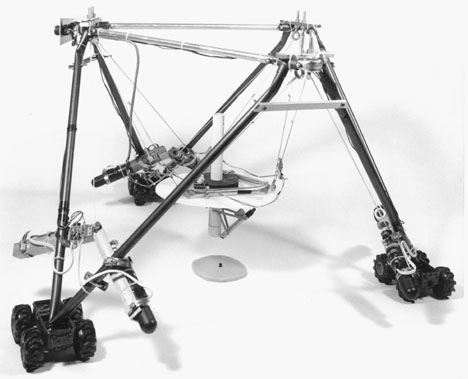
\includegraphics[width=.40\linewidth]{./chapter0/figures/robot_cdpr_crane.jpg}}
    \caption{\footnotesize Deux configurations possibles pour un robot 
parallèle 
à câble}
\label{intro:fig5}
\end{figure}

Une caractéristique particulière des manipulateurs parallèles à câbles qui les 
différencie des manipulateurs parallèles classiques est la {\bf non-rigidité 
des 
jam\-bes}. Sous certaines conditions, un ou plusieurs câbles peuvent être 
détendus, ce qui a pour effet qu'ils n'exercent plus de force sur la 
plate-forme. Nous reviendrons plus loin sur ce point essentiel.

Comparativement donc aux robots parallèles classiques, les robots parallèles à 
câbles présentent les caractéristiques suivantes :
\begin{itemize}
 \item la structure parallèle permet de conserver les propriétés de 
compensation 
des erreurs, de répartition des charges et des efforts, de coopération des 
chaînes cinématique pour l'exécution d'un mouvement
 \item l'espace de travail est considérablement agrandi par rapport aux robots 
parallèles à jambes rigides
 \item l'équipage mobile est très léger, ce qui favorise la dynamique
 \item le comportement des câbles (non-déformables, élastiques, pesants, \dots) 
peut complexifier s\'erieusement le modèle du robot
 \item l'unilatéralité des forces implique que nous puissions nous retrouver 
dans une situation avec un ou plusieurs câbles détendus, ce qui doit être pris 
en compte dans le contrôle.
\end{itemize}

Après avoir introduit quelques notations, nous allons à présent décrire les 
modèles géométriques direct et inverse, cinématiques ainsi que l'équilibre 
statique pour les robots parallèles à câble. Ceci nous permettra de lister tant 
que faire se peut l'ensemble des difficultés posées par ce type de manipulateur 
et auxquelles nous avons été confrontées dans le cadre de nos recherches.

\subsection{Notations} \label{chap0-1-0}

\begin{figure}[!ht]
\centering
\def\svgwidth{.85\linewidth}
\input{./chapter0/figures/notation_schema.pdf_tex}
\end{figure}

\begin{itemize}
 \item $R_b$ : référentiel de la base
 \item $R_e$ : référentiel de l'organe terminal
 \item $A_i$ : point d'attache du $i^{\hbox{ème}}$ câble à la base ; le terme 
de 
{\it point de sortie} sera également utilisé.
 \item $B_i$ : point d'attache du $i^{\hbox{ème}}$ câble à l'organe terminal
 \item $C$ : un point arbitraire de l'organe terminal utilisé comme référence 
pour sa position
 \item $\rho_i$ : longueur réelle du câble $i$
 \item $l_i$ : longueur déroulée du câble $i$
 \item $\boldmath {\mathcal F}$ : vecteur des forces exercées sur l'organe 
terminal
 \item $\bf J$ : jacobienne du robot
\end{itemize}
Enfin, on utilisera la notation ${\bf J}^{-1}$ pour exprimer la jacobienne 
inverse, et ${\bf J}^{-T}$ sera utilisé comme raccourci de notation pour sa 
transposée.

Sauf mention du contraire, {\bf nous supposerons dans la suite que les câbles 
sont non-pesants et non-élastiques}, ce qui est une hypothèse adéquate pour le 
robot que nous avons utilisé.

\subsection{Modèle géométrique inverse} \label{chap0-1-1}

Le modèle géométrique inverse consiste à déterminer les coordonnées 
articulaires 
à partir des coordonnées opérationnelles. Dans le cas des robots parallèles à 
câbles, les coordonnées articulaires correspondent aux longueurs $\rho$ des 
câbles. Lorsque ceux-ci sont tendus, cette longueur doit être égale à la 
distance entre les points de sortie ${\bf A}_i$ et le point d'attache à la 
plate-forme ${\bf B}_i$. Dans le cas où le câble est détendu, la longueur sera 
supérieure à cette distance (Fig.\ref{intro:fig6view0}).\\

%%%%%% une figure différente
\begin{figure}[!ht]
  \centering
      \subfloat[Forme d'un câble dont la tension serait 
nulle]{\label{intro:fig6view0}
\def\svgwidth{.45\linewidth}
\input{./chapter0/figures/nulltensionwire.pdf_tex}} 
\hfill
\subfloat[Câble élastique sur lequel est appliquée une tension positive : 
la longueur réelle diffère de la longueur déroulée]{\label{intro:fig6view1}
\def\svgwidth{.45\linewidth}
\input{./chapter0/figures/positivetensionwire.pdf_tex}}
    \caption{\footnotesize{Dans le cas d'un câble détendu (tension nulle), la 
longueur déroulée (en bleu pointill\'e) sera supérieure à la distance entre les 
deux points d'attache (en rouge plein) ; de plus, la forme du câble sera telle 
qu'il y a risque d'intersection avec d'autres câbles, l'environnement, \dots. 
Dans le cas d'un câble élastique tendu (tension strictement positive), la 
longueur déroulée $l_i$ (en bleu pointill\'e) sera inférieure à la 
distance entre les points d'attache correspondant à la longueur réelle du 
câble $\rho_i$ (en rouge plein)}}
\label{intro:fig6}
\end{figure}

Nous partons donc des relations suivantes :
\begin{eqnarray}
\rho_i &=& ||{\bf A}_i {\bf B}_i||, \hbox{ si } \tau_i > 0 \\ 
\rho_i &\geq& ||{\bf A}_i {\bf B}_i||, \hbox{ si } \tau_i = 0
\label{intro:eq1}
\end{eqnarray}

Comme on le voit, il n'est pas possible d'obtenir les longueurs $\rho_i$ sans 
prendre en compte les tensions $\tau_i$. Dès lors, tout comme dans l'approche 
développée par \cite{2010:Carricato.Merlet}, nous parlerons donc de modèle 
géométrico-statique inverse, requérant l'étude de l'équilibre statique.

\subsection{Equilibre statique} \label{chap0-1-2}

On dit d'un solide au repos qu'il est en équilibre statique lorsque l'ensemble 
des forces extérieures $\mathcal {\bf F}_{\hbox{ext}_i}$ qui s'exercent sur lui 
s'annulent, ce qui se traduit par la relation suivante :
\begin{equation}
\sum_i \boldmath {\mathcal F}_{\hbox{ext}_i} = {\bf 0}
\label{intro:eq2}
\end{equation}

Sous l'hypothèse que les forces mécaniques de frottement et de résistance 
peuvent être ici négligées, nous considérons uniquement la force de gravité 
exercée sur la plate-forme ainsi que les efforts exercés par chacun des câbles.

La direction dans laquelle un câble de longueur $\rho_i$ relié à la base au 
point ${\bf A}_i$ et à la plate-forme au point ${\bf B}_i$ exerce une force sur 
la plate-forme est donnée par le vecteur ${\bf u}_i = \frac{{\bf A}_i{\bf 
B}_i}{\rho_i}$. On peut dès lors définir pour ce câble un torseur ${\bf W}_i$ 
correspondant aux efforts et couples exercés par celui-ci sur la plate-forme :
\begin{equation}
{\bf W}_i = -({\bf u}_i^T, (p_i \times {\bf u}_i)^T)^T
\label{intro:eq3}
\end{equation}
où $p_i$ est un vecteur allant d'un premier point de référence arbitraire 
$C$ localisé sur la plate-forme au point ${\bf B}_i$. La force exercée par le 
câble sur la plate-forme est alors $ \tau_i {\bf W}_i$ , où $\tau_i$ est un 
scalaire positif représentant l'intensité de la tension.

Soit ${\bf W}_g$ le torseur indiquant la direction dans laquelle la gravité est 
exercée dans le référentiel choisi, pour $n$ câbles, (Equ.\ref{intro:eq2}) 
s'écrit pour nous :
\begin{equation}
\begin{bmatrix}
 {\bf W}_1 & {\bf W}_2 & \dots & {\bf W}_n & {\bf W}_g
\end{bmatrix}
\begin{bmatrix}
 \tau_1 \\ \tau_2 \\ \dots \\ \tau_n \\ \hbox{mg}
\end{bmatrix}
= {\bf 0}
\label{intro:eq4}
\end{equation}

En posant ${\bf \tau} = (\tau_1, \tau_2, \dots, \tau_n)^T$, ${\bf W}$ la 
matrice 
$6 \times n$ dont les colonnes sont les $n$ torseurs ${\bf W}_i$, et en isolant 
$\mathcal {\bf F} =  \hbox{mg} {\bf W}_g$ modélisant la force de gravité, la 
relation (Equ.\ref{intro:eq4}) s'écrit également :
\begin{equation}
\mathcal {\bf F} + {\bf W} \tau = {\bf 0}
\label{intro:eq5a}
\end{equation}

soit  
\begin{equation}
\mathcal {\bf F} = {\bf J}^{-T} {\bf \tau}
\label{intro:eq5b}
\end{equation}
où ${\bf J}^{-1} = - {\bf W}^T$ est une matrice que l'on appelle {\it 
jacobienne 
inverse}.

\subsection{Modèle géométrico-statique inverse (ou {\it MGSI})} 
\label{chap0-1-3}


Connaissant les paramètres de pose de la plate-forme, on veut en déduire les 
longueurs supposées $\rho_i$ des câbles : c'est le modèle géométrique inverse. 
Dans le cas où nous avons $m \geq 6$ câbles, connaissant la pose 
${\bf B}$ et les points de sorties ${\bf A}_i$, on peut calculer les longueurs 
$\rho_i$. Si $m = 6$, la solution de l'équilibre statique est unique, 
l'\'equilibre statique possède sinon en théorie une infinité de solution (nous 
ne devons toutefois consid\'erer que les ensembles de solutions pour lesquelles 
les $\tau_i$ sont tous strictement positifs).

Il est cependant n\'ecessaire d'envisager les possibilit\'es pour lesquelles 
moins de $6$ c\^ables sont en tension. Nous avons d\`es lors $m < 6$, et nous 
ne pouvons donc plus sp\'ecifier que $m$ degr\'es de libert\'es : il faut alors 
faire intervenir la statique afin de calculer les $6-m$ degr\'es de libert\'e. 
Plusieurs m\'ethodes s'offrent \`a nous, dont :
\begin{itemize}
 \item par r\'esolution inverse de l'\'equilibre statique, on \'elimine les 
$\tau$ correspondant aux c\^ables mous, puis on reporte dans les \'equations du 
mod\`ele g\'eom\'etrique inverse, ce qui nous donne $6-m$ \'equations.
\item L'équilibre statique est vérifié 
uniquement si l'ensemble des déterminants $m+1 \times m+1$ de la matrice ${\bf 
W}$ sont nuls \cite{carricato_merlet2013}. Si tous les $\tau_i$ sont 
strictement positifs, le modèle géométrico-statique possède alors une solution, 
mais correspondant à un mode dégradé du système.
\end{itemize}


\subsection{Modèle géométrico-statique direct}\label{chap0-1-4}

Résoudre le modèle géométrique direct consiste à calculer les coordonnées 
opéra\-tionnelles à partir de la donnée des coordonnées articulaires. Il s'agit 
donc dans le contexte d'un robot parallèles à câbles de déduire la pose de la 
plate-forme (position et orientation) à partir des longueurs des câbles. C'est 
un problème qui a posé de nombreux défis mathématiques et algorithmiques dans 
le 
cas des robots parallèles rigides \cite{merlet1997robots}, et nous allons voir 
qu'il peut \^etre plus complexe dans le cas des CDPR.

On distinguera les cas suivants :
\begin{itemize}
  \item $m > 6$ : dans le cas o\`u nous avons $m > 6$ c\^ables, les inconnues 
sont les $6$ param\`etres de pose de $\bf X$. Nous avons $6 > m$ \'equations 
fournies par le mod\`ele g\'eom\'etrique. Le syst\`eme \`a r\'esoudre ne 
poss\`ede cependant en g\'en\'eral aucune solution : on en d\'eduit alors qu'un 
ou plusieurs c\^ables sont mous, ce que l'\'etude de l'\'equilibre statique 
nous permettront de v\'erifier. On cherche alors les solutions valides pour 
$m-1$ c\^ables.
  \item $m = 6$ : cette situation peut \^etre ramen\'ee \`a son 
\'equivalent pour les robots parall\`eles classiques ; dans ce cas, les 
\'equations g\'eom\'etriques et celles de la statique sont d\'ecoupl\'ees. La 
g\'eom\'etrie nous donne les poses $\bf X$, et on v\'erifie la validit\'e de 
celles-ci avec la statique.
  \item $m < 6$ : ici, nous avons $6$ inconnues (les param\`etres de pose $\bf 
X$). Or, le mod\`ele g\'eom\'etrique ne fournit que $m < 6$ \'equations. On 
compl\`etera d\`es lors le syst\`eme avec les \'equations de l'\'equiibre 
statique. Dans cette nouvelle situation, nous avons $6 + m$ inconnues ($6$ 
param\`etres de pose et $m$ tensions) pour $6 + m$ \'equations (dont $m$ sont 
fournies par le mod\`ele g\'eom\'etrique et $m$ par l'\'equilibre statique). On 
obtient alors bien un syst\`eme carr\'e, mais dont le nombre d\'equations est 
tr\`es sup\'erieur \`a son \'equivalent pour les robots parall\`eles \`a jambes 
rigides. Dans le cas $m = 5$, on a en effet $11$ \'equations pour les robots 
parall\`eles \`a c\^ables, contre $5$ pour les robots parall\`eles rigides.
Toutefois, le syst\`eme de $n+6$ \'equations \`a $n+6$ inconnues ainsi obtenu 
n'est valide qu'`a la condition que tous les c\^ables soient tendus, soit que 
$\forall i \in [0,m], \rho_i = ||{\bf A}_i{\bf B}_i||$. On ne peut jamais 
exclure que la plate-forme soit dans une pose pour la\-quelle $\exists i \in 
[1,m], \rho_i > ||{\bf A}_i{\bf B}_i||$. Dans ce cas, une des \'equations du 
mod\`ele g\'eom\'etrique ne sera plus valide. Il faut donc consid\'erer tous 
les cas avec $6+m-p$ \'equations ($p \in [1, m-1]$) et v\'erifier $p$ fois la 
validit\'e des r\'esultats ($\rho_i > ||{\bf A}_i{\bf B}_i||$, $\tau_i > 0$). 
\end{itemize}

Ce qui doit \^etre retenu ici est qu'il est difficile lors d'un déplacement de 
prévoir à l'avance quels câbles seront en tension en chaque point de la 
trajectoire ainsi que la valeur des tensions.

Ce point, très peu mentionné dans la littérature, est un des inconvénients 
majeurs de l'utilisation des robots parallèles à câbles. Le premier chapitre de 
ce travail montrera qu'il est toutefois possible d'élaborer une stratégie 
prenant ce problème en compte pour améliorer le contrôle et la stabilité du 
système pour la grande majorité des situations.

\subsection{Modèle cinématique}\label{chap0-1-5}

Le modèle cinématique consiste à établir une relation entre les 
vitesses articulaires ${\bf \dot \Theta}$ et la vitesse (translation et 
angulaire) de la plate-forme $\bf \Omega$.

Nous avons vu que le vecteur ${\bf A}_i{\bf B}_i$ peut être calculé de deux 
manières différentes :
\begin{itemize}
 \item connaissant la pose de la plate-forme et sa géométrie, les coordonnées 
de 
${\bf B}_i$ sont données ; ${\bf A}_i$ étant connu par la géométrie du robot, 
on 
peut définir une fonction $H_1$ dépendante uniquement de la pose telle que :
\begin{equation}
{\bf A}_i{\bf B}_i = H_{1_{|i}}({\bf X})
\label{intro:eq6}
\end{equation}
 \item à partir des coordonnées articulaires (et éventuellement de la pose si 
l'intervention de l'équilibre statique est requise), le {\it MGSD} permet de 
définir la relation suivante :
\begin{equation}
{\bf A}_i{\bf B}_i = H_{2_{|i}}({\bf X}, {\bf \Theta})
\label{intro:eq7}
\end{equation}
\end{itemize}
 
Si ${\bf AB}$ est le vecteur composé des différents ${\bf A}_i{\bf B}_i$, alors 
on obtient en combinant (Equ.\ref{intro:eq6}) et (Equ.\ref{intro:eq7}) :
\begin{equation}
\begin{matrix}
{\bf AB} &=& H_1({\bf X}) \\
{\bf AB} &=& H_2({\bf X}, {\bf \Theta}) \\
\Longrightarrow & & H_1({\bf X}) = H_2({\bf X}, {\bf \Theta})
\end{matrix}
\label{intro:eq8}
\end{equation}

En différentiant (Equ.\ref{intro:eq8}), on obtient :
\begin{equation}
\frac{\partial H_1}{\partial {\bf X}} \frac{\partial {\bf X}}{\partial t} 
=  \frac{\partial H_2}{\partial {\bf X}} \frac{\partial {\bf X}}{\partial t} + 
\frac{\partial H_2}{\partial {\bf \Theta}} \frac{\partial {\bf 
\Theta}}{\partial t}
\label{intro:eq9}
\end{equation}

soit :

\begin{equation}
\dot {\bf \Theta} = \left ( \frac{\partial H_2}{\partial {\bf \Theta}} \right 
)^{-1} \left (\frac{\partial H_1}{\partial {\bf X}} - \frac{\partial 
H_2}{\partial {\bf X}} \right ) \dot {\bf X}
\label{intro:eq10}
\end{equation}

Si $\left ( \frac{\partial H_2}{\partial {\bf \Theta}} \right )$ est bien 
inversible, nous pouvons définir une matrice ${\bf J}^{-1}$ de manière à 
obtenir la 
relation suivante :
\begin{equation}
\dot {\bf \Theta} = {\bf J}^{-1} \dot {\bf X}
\label{intro:eq11}
\end{equation}

Toutefois, le vecteur $\dot {\bf X}$ ainsi d\'etermin\'e ne correspond pas \`a 
$\bf \Omega$, il d\'epend de la param\'etrisation choisie pour les param\`etres 
de pose. En particulier, si nous utilisons les angles d'Euler pour param\'etrer 
l'orientation de la plate-forme, nous pouvons exprimer la v\'elocit\'e d'un 
point ${\bf B}$ en fonction de la vitesse d'un point ${\bf C}$ de r\'ef\'erence 
de la plate-forme avec la relation suivante :
\begin{equation}
{\bf v_B} = {\bf v_C} + {\bf BC} \times {\bomega_c}
\label{intro:eq11b}
\end{equation}
o\`u $\bf V_C$ d\'enote la v\'elocit\'e de la plate-forme au point ${\bf C}$, 
et ${\bomega_C}$ le vecteur des v\'elocit\'es angulaires.

Ainsi, comme ${\bf A}_i$ est fix\'e, nous avons pour le c\^able $i$ :
\begin{equation}
\dot { {\bf A}_i{\bf B}_i } = {\bf v_C} + {\bf B}_i{\bf C} \times {\bomega_c}
\label{intro:eq11c}
\end{equation}

En posant :
\begin{equation}
\dot {\bf X} = \begin{matrix}
                {\bf V_C} \\
		{\bomega_C}
               \end{matrix}
\label{intro:eq11d}
\end{equation}
nous construisons ainsi une relation entre les vitesses articulaires et les 
vitesses de translation et d'orientation, ces derni\`eres param\'etr\'ees par 
les angles d'Euler.

La matrice ${\bf J}^{-1}$ ainsi construite est appelée {\it Jacobienne 
inverse param\'etr\'e} par les angles d'Euler. On notera qu'elle dépend à la 
fois des paramètres de pose et des coordonnées articulaires : il requiert d\`es 
lors la r\'esolution des mod\`ele g\'eom\'etriques direct et inverse.

\section{Les robots N-1} \label{chap0-2}

On parle de configuration N-1 pour un robot parall\`ele \`a c\^ables en 
configuration suspendue lorsque l'ensemble des c\^ables sont reli\'es \`a la 
plate-forme en un m\^eme point ${\bf B}$. Cette architecture pr\'esente les 
caract\'eristiques suivantes :
\begin{itemize}
  \item puisque l'ensemble des points ${\bf B}_i$ sont confondus, le contr\^ole 
en orientation n'est plus possible : c'est donc une architecture d\'edi\'ee aux 
d\'eplacements en translation. Entre autres avantages, nous n'avons plus \`a 
nous pr\'eoccuper des inerf\'erences entre c\^ables.
  \item si $N > 3$, seuls trois c\^ables au plus seront en tension positive et 
permettront de contr\^oler les d\'eplacements de la plate-forme ; le cas N-4 
sera expliqu\'e en d'etail \`a l'occasion du chapitre consacr\'e aux 
configurations de c\^ables.
  \item les tensions n'\'etant r\'eparties qu'entre au plus trois c\^ables, 
l'ajout de c\^ables suppl\'ementaires ne peut servir \`a soulager les autres 
c\^ables. Par contre, il est possible d'envisager de choisir le meilleur 
triplet 
en fonction d'un crit\`ere donn\'e, parmi tous ceux que l'utilisation de $N>3$ 
c\^ables rend possible ($4$ triplets au plus pour $4$ c\^ables, $10$ pour $5$ 
c\^ables, $20$ pour $6$ c\^ables, $\cdots$). De plus, l'utilisation de c\^ables 
suppl\'ementaires permet d'augmenter l'espace de travail du robot, lorsque le 
point d'attache du c\^able ajout\'e est plac\'e en dehors de celui-ci.
\end{itemize}

\subsection{Mod\`eles g\'eom\'etriques}

{\bf MGSD :}\\

\begin{figure}[!ht]
  \centering
    \def\svgwidth{.85\linewidth}
      \input{./chapter0/figures/MGDN1.pdf_tex}
    \caption{\footnotesize{Repr\'esentation des points d'intersection des 
trois sph\`eres de centre ${\bf A}_i$ (resp. ${\bf A}_j$, ${\bf A}_k$) et de 
rayon $\rho_i$ (resp. $\rho_j$, $\rho_k$). Dans ce cas pr\'ecis, la solution la 
plus haute est haut-dessus du plan contenant les points ${\bf A}_i$, ${\bf 
A}_j$ et ${\bf A}_k$ : elle ne peut se retrouver en \'equilibre statique, 
aucun c\^able ne pouvant fournir une force oppos\'ee \`a la force de 
gravit\'e.}}
\label{intro:fig6b}
\end{figure}

Soient $N$ c\^ables dont nous connaissons les longueurs $\rho_0, \cdots, 
\rho_{N-1}$. Puisque nous n'avons que $3$ c\^ables au plus en tension, nous 
commen\c cons par r\'esoudre le mod\`ele g\'eom\'etrique pour chaque 
triplet de c\^ables. Ne contr\^olant pas les rotations, les param\`etres de 
pose sont uniquementles coordonn\'ees dans l'espace. D\`es lors, nous avons $3$ 
inconnues, et $3$ \'equations. Les solutions fournies par la r\'esolution du 
syst\`eme seront ensuite valid\'ees par l'\'etude de l'\'equilibre statique. 
S'agissant des points d'intersections de trois sph\`eres de centre ${\bf A}_i$ 
et de rayon $\rho_i$, il y aura au maximum deux solutions pour chaque triplet 
de c\^ables, dont une au moins ne respectera pas l\'equilibre statique. Il y a 
donc pour chaque triplet de c\^ables au plus une pose valide \ref{intro:fig6b}.

Il faut ensuite v\'erifier que nous n'ayons pas une pose valide avec moins de 
$3$ c\^ables en tension : dans ce cas, nous avons deux \'equations donn\'ees 
par la g\'eom\'etrique, pour les trois inconnues que constituent les 
param\`etres de poses. En compl'etant avec la statique qui nous donne 3 
\'equations pour deux inconnues qui sont les tensions dans les deux c\^ables 
test\'es. Toutefois, les trois \'equations de la statique seront lin\'eairement 
d\'ependante. On ajoutera donc une derni\`ere \'equation de contrainte 
stipulant que la pose doit se trouver sur la projection verticale de la droite 
issue des points ${\bf A}_i$ et ${\bf A}_j$ test\'es. On proc\`edera enfin de 
m\^eme pour l'\'etude des cas \`a un seul c\^able en tension positive. \\


{\bf MGSI :}\\

Le mod\`ele g\'eom\'etric0-statique indirect est relativement simple dans ce 
contexte. Connaissant les param\`etres de pose, les longueurs de c\^ables 
peuvent \^etre imm\'ediatement d\'eduite \`a partir de la relation 

\begin{equation}
\rho_i = ||{\bf A}_iB||^2
\label{intro:eq11a}
\end{equation}

La solution ainsi d\'etermin\'ee est unique du point de vue de sa localisation 
dans l'espace, mais peut correspondre \`a plusieurs situations de triplets de 
c\^ables en tension.\\

{\bf Cin\'ematique :}\\

Si nous d\'erivons la relation pr\'ec\'edente \ref{intro:eq11a}, nous avons :
\begin{equation}
2 \rho_i \partial \rho = 2 x \partial x + 2 y \partial y + 2 z \partial z
\label{intro:eq11a2}
\end{equation}
avec ${\bf A}_i{\bf B} = {\bf X}_i = (x, y, z)$.

D\`es lors, on obtient :
\begin{equation}
\partial \rho = \frac x \rho \partial x + \frac y \rho \partial y + \frac y 
\rho \partial z
\label{intro:eq11a3}
\end{equation}

On en d\'eduira pour le c\^able $i$ la ligne correspondante de la 
matrice Jaco\-bienne inverse :
\begin{equation}
{\bf J}^{-1}_i = 
\begin{bmatrix}
\frac {{\bf B}_x - {\bf A}_{i_x}} {\rho_i} & \frac {{\bf B}_y - {\bf A}_{i_y}} 
{\rho_i} & \frac {{\bf B}_z - {\bf A}_{i_z}} {\rho_i} 
\end{bmatrix}
\label{intro:eq11a4}
\end{equation}



\subsection{{\tt Marionet-Assist}} \label{chap0-2-2}

Les {\tt Marionet} sont une classe de robots à câbles développés par l'EPI 
Hephaistos pour des applications diverses \cite{merlet2010marionet} :
\begin{itemize}
 \item {\tt Marionet-Crane} (Fig.\ref{intro:fig7view0}) : intervention à grande 
échelle pour des opé\-rations de sauvetage dans des situations de catastrophe 
naturelle
 \item {\tt Marionet-VR} (Fig.\ref{intro:fig7view1}) : utilisation en dans des 
environnements de r\'ealit\'e virtuel en tant que g\'en'erateur de mouvement et 
comme interface haptique. 
 \item {\tt Marionet-Rehab} (Fig.\ref{intro:fig7view2}) : rééducation et 
assistance à la personne ; pouvant atteindre des vitesses allant jusqu'à 
100m/s, 
il est également possible de l'utiliser pour des opérations de transfert 
ultra-rapides
 \item {\tt Marionet-School} (Fig.\ref{intro:fig7view3}) : pédagogie et 
diffusion ; ces robots sont utilisés entre autres pour illustrer de manière 
ludique des propriétés géométriques et mathématiques auprès des publics jeunes
\end{itemize}

\begin{figure}[!ht]
  \centering
    \subfloat[{\tt Marionet-Crane} : son espace de 
travail peut aller jusqu\`a $15m \times 15m \times 
15m$, et la l\'eg\`eret\'e de son \'equipement garantit 
un d\'eploiement rapide]{\label{intro:fig7view0}
    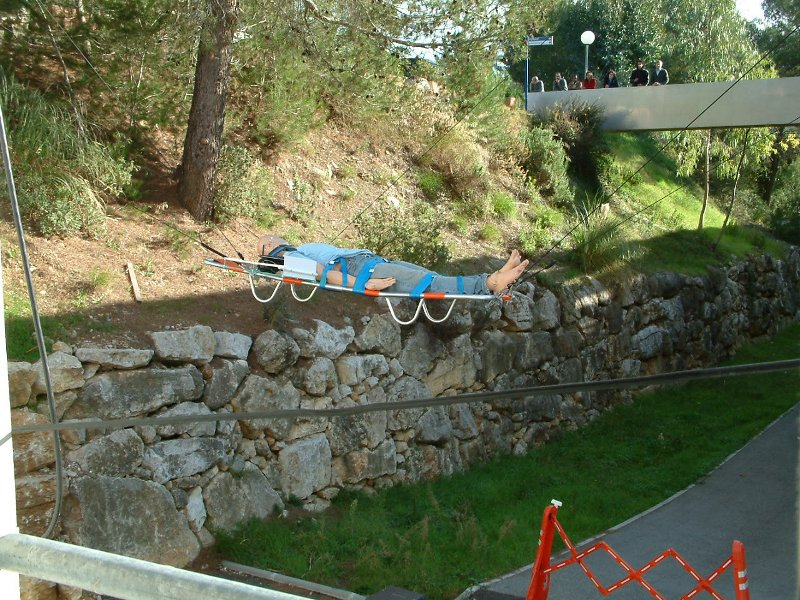
\includegraphics[width=.42\linewidth]{./chapter0/figures/marionet03.jpg}}  
\hfill
    \subfloat[{\tt Marionet-VR} : utilise des 
actionneurs lin\'eaires pour une pr\'ecision accrue 
dans un espace de travail de $6m \times 5m \times 
3m$]{\label{intro:fig7view1}
    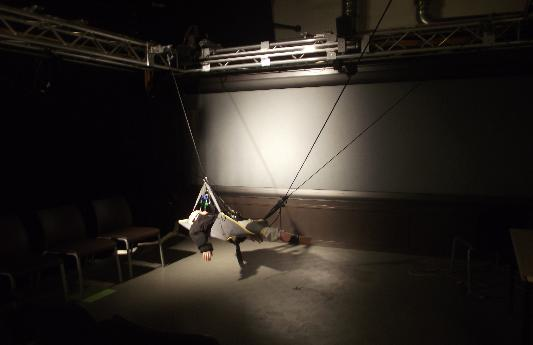
\includegraphics[width=.48\linewidth]{./chapter0/figures/marionet05.jpg}} \\
    \subfloat[{\tt Marionet-Rehab} : utilise des actionneurs lin\'eaires pour 
de la mesure de mouvements (mode passif) et des t\^aches de 
r\'ehabilitation (mode actif)]{\label{intro:fig7view2}
    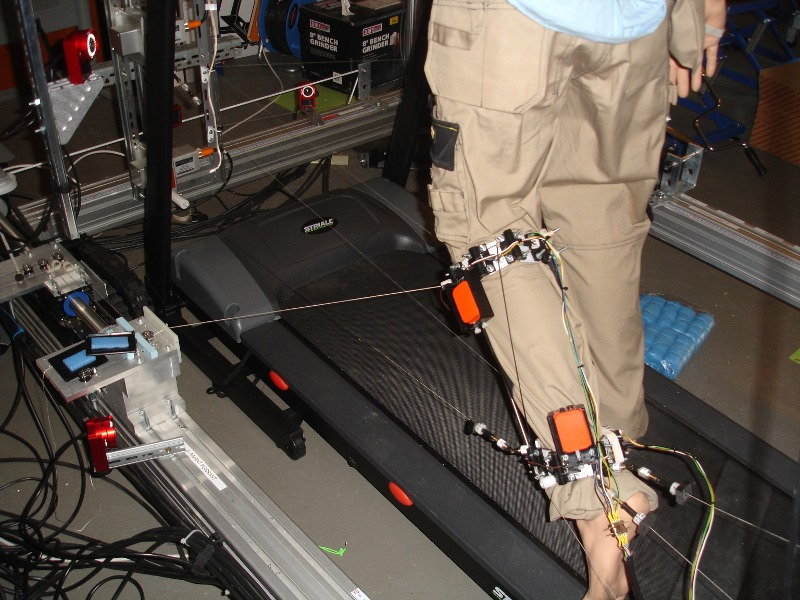
\includegraphics[width=.45\linewidth]{./chapter0/figures/marionet01.jpg}} 
\hfill
    \subfloat[{\tt Marionet-School} : ais\'ement 
transportable et d\'eployable, il est utilis\'e pour des interventions 
p\'edagogiques]{\label{intro:fig7view3}
    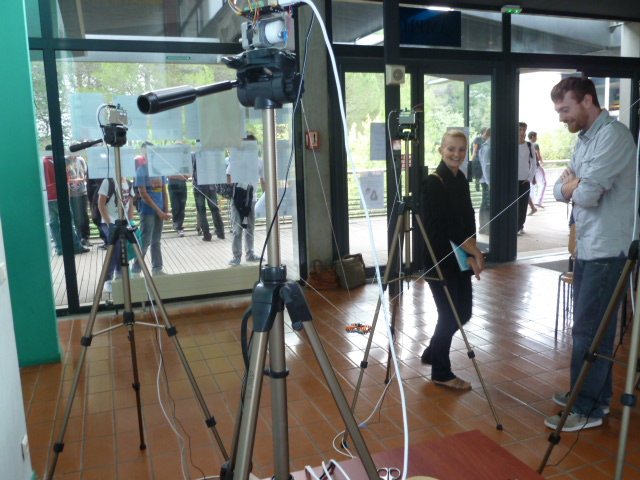
\includegraphics[width=.45\linewidth]{./chapter0/figures/marionet02.jpg}}
    \caption{\footnotesize{Exemples d'utilisation des robots {\tt Marionet}}}
\label{intro:fig7}
\end{figure}

Le robot {\tt Marionet-Assist} a été développé dans un objectif d'assistance 
aux 
personnes à mobilités réduites, et plus spécifiquement dans une démarche 
d'amélio\-ration de l'autonomie des publics concernés. Il doit pouvoir répondre 
à des situations tout aussi diverses que :
\begin{itemize}
 \item soutien ponctuelle au déplacement pour une personne âgée expérimentant 
une fatigue articulaire (par exemple pour la passage de la baignoire) 
(Fig.\ref{intro:fig8view0})
 \item aide au transfert d'une position à une autre pour une personne (des 
toilettes au fauteuil par exemple) 
(Fig.\ref{intro:fig8view1})
 \item aide aux aidants pour le transfert de personnes atteintes de 
tétraplégie (déplacement du lit vers un fauteuil par exemple) afin de r\'eduire 
la p\'enibilit\'e de leur t\^ache. 
(Fig.\ref{intro:fig8view2})
\end{itemize}

\begin{figure}[htp]
  \centering
  \subfloat[Simple soutien au déplacement dans une pièce de 
vie]{\label{intro:fig8view0}
  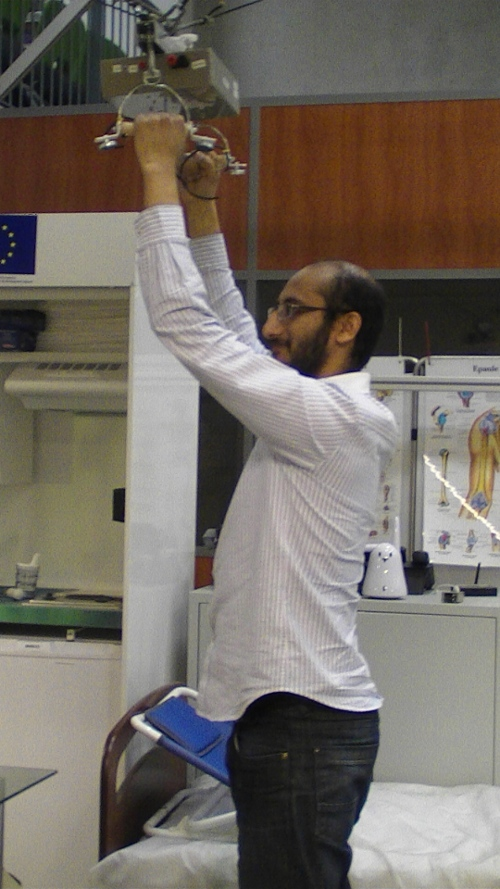
\includegraphics[width=.2\linewidth]{./chapter0/figures/case01.jpg}} \hfill
  \subfloat[Transfert de position assise/levé]{\label{intro:fig8view1}
  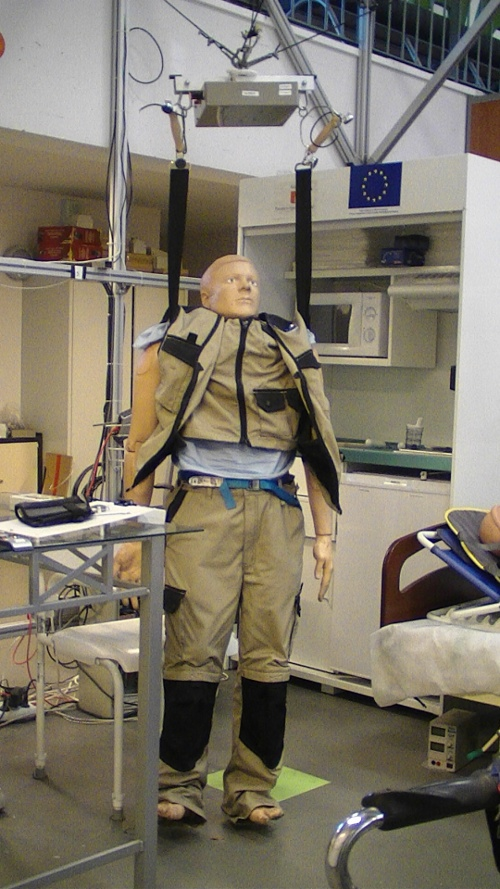
\includegraphics[width=.2\linewidth]{./chapter0/figures/case02.jpg}} \hfill
  \subfloat[Déplacement autonome d'un lieu de vie (lit) vers un dispositif de 
déplacement (fauteuil)]{\label{intro:fig8view2}
  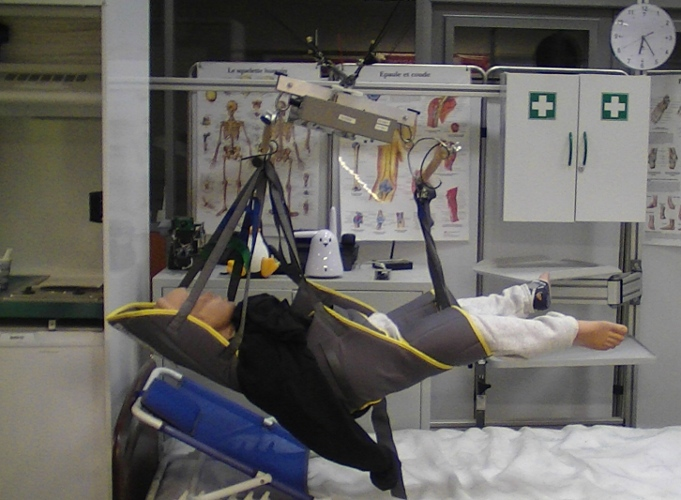
\includegraphics[width=.48\linewidth]{./chapter0/figures/case03.jpg}} \hfill
    \caption{\footnotesize{Différents types de fragilités motrices dans des 
situation de la vie quotidienne}}
\label{intro:fig8}
\end{figure}

Un dispositif répondant à ces impératifs doit présenter les caractéristiques 
suivantes :
\begin{itemize}
 \item pouvoir supporter des charges correspondant au poids d'une personne
 \item avoir un espace de travail équivalent à la taille d'une pièce de vie
 \item être léger et suffisamment discret et modulaire pour ne pas bouleverser 
l'environnement de l'utilisateur
 \item avoir une précision suffisante pour permettre un positionnement 
garantissant la sécurité, l'efficacité et le confort des opérations de 
transfert 
et d'attachement/détachement de l'utilisateur à la plate-forme.
\end{itemize}

Le choix d'utilisation d'un robot parallèle à câbles semble donc le plus 
compatible avec l'ensemble de ces exigences. {\tt Marionet-Assist} a ainsi été 
conçu et déployé dans un appartement-témoin 
(Fig.\ref{intro:fig10view0},\ref{intro:fig10view1}) situé dans les locaux 
de l'INRIA. Les câbles permettant le contrôle de la plate-forme sont fixés au 
plafond de l'appartement. Dans sa configuration actuelle, {\tt Marionet-Assist} 
est équipé de $4$ câbles, mais peut en contrôler jusqu'à $6$. Plusieurs 
stratégies sont envisageables au niveau des points de fixation sur la 
plate-forme :
\begin{itemize}
 \item les points d'attaches des câbles sont tous différents, il est alors 
possible avec $n$ câbles de contrôler $n$ degrés de liberté. Cette 
configuration.
sera notée $N-N$ (Fig.\ref{intro:fig9view0}).
 \item les câbles sont attachés en un même point à la plate-forme : il est 
posible à partir de $3$ câbles de contrôler les déplacement en translation de 
la plate-forme, mais plus son orientation ; l'utilisation de plus de $3$ câbles 
permet alors d'augmenter la taille de l'espace de travail. On parle dans ce cas 
de configuration N-1. 
(Fig.\ref{intro:fig9view1}).
 \item certains câbles seulement sont attachés en un même point sur la 
plate-forme. Dans le cas par exemple d'une disposition pour laquelle $3$ câbles 
sont atttachés en un même point $B_0$ et un quatrième câble relié à la 
plate-forme en un point $B_1$, cette configuration sera notée 4-3-1 
(Fig.\ref{intro:fig9view2}).
\end{itemize}

\begin{figure}[htp]
  \centering
  \subfloat[Configuration 4-4 : chaque câble est relié à la plate-forme en un 
point distinct]{\label{intro:fig9view0}
  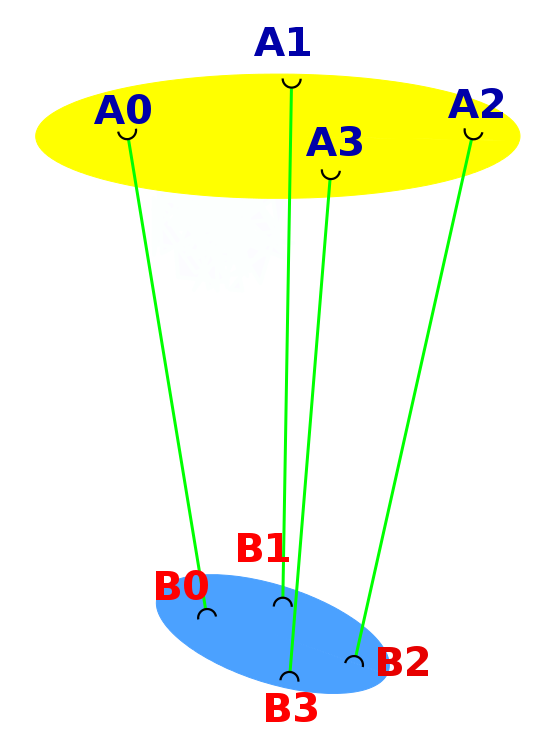
\includegraphics[width=.3\linewidth]{./chapter0/figures/cfg_44.png}} \hfill
  \subfloat[Configuration 4-1 : Les $4$ câbles sont reliés à la plate-forme un 
un seul point]{\label{intro:fig9view1}
  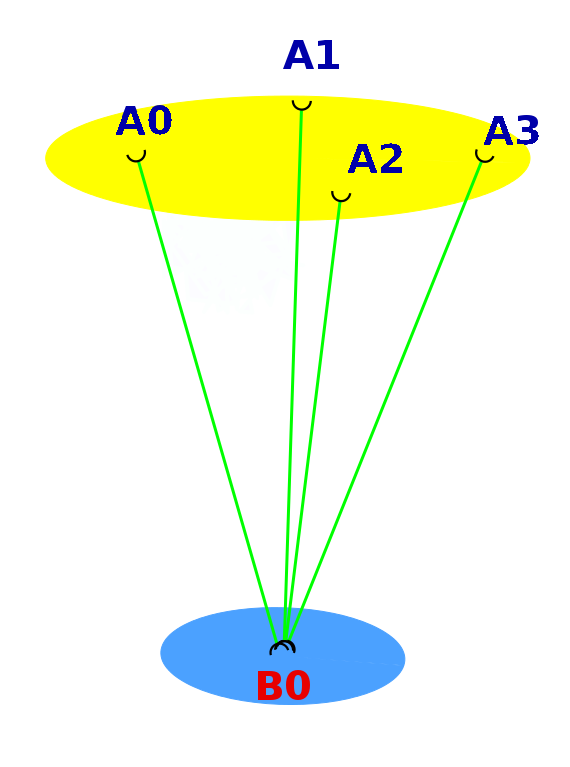
\includegraphics[width=.3\linewidth]{./chapter0/figures/cfg_41.png}}
  \subfloat[Configuration 4-3-1 : $3$ câbles sont reliés à la plate-forme en un 
même point, le quatrième est relié en un point distinct]{\label{intro:fig9view2}
  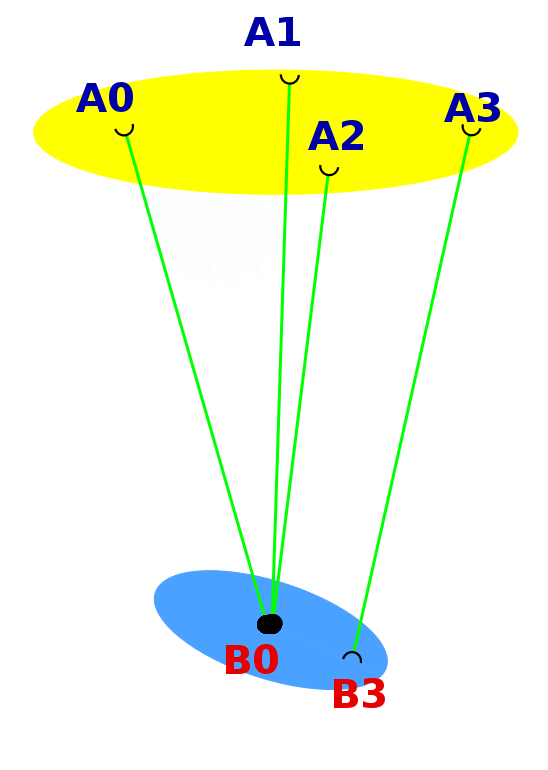
\includegraphics[width=.3\linewidth]{./chapter0/figures/cfg_431.png}} \hfill
    \caption{\footnotesize{Exemples de configurations avec $4$ câbles}}
\label{intro:fig9}
\end{figure}

Pour l'ensemble des expériences menées dans le cadre de ce travail, nous avons 
utilisé la configuration $4-1$ (Fig.\ref{intro:fig10view2}) qui nous permet de 
contrôler les déplacements en translation, le quatrième c\^able ayant été 
ajouté pour augmenter la taille l'espace de travail de manière à pouvoir se 
déplacer dans la quasi-totalité de l'appartement-témoin. Pour un triplet de 
c\^ables en tension, il est facile de montrer que l'\'equilibre statique est 
satisfait si le point ${\bf B}$ \`a sa projection dans le plan des ${\bf 
A}_i,{\bf A}_j,{\bf A}_k$ \`a l'int\'erieur du triangle constitu\'e par ces 
trois points. La figure (Fig.\ref{intro:fig11}) montre alors l'espace de 
travail 
atteignable pour chaque triplet de câbles en tension : on note qu'en tout point 
dont la projection verticale ne se trouve pas sur l'une des deux diagonales 
définies par les points $(A_0-A_2)$ et $(A_1-A_3)$, il existe pour chaque pose 
deux configurations possibles avec trois câbles en tension. Si la projection se 
trouve sur une diagonale, i lexiste une configuration qui a deux c\^ables en 
tension, \`a l'exception de l'intersection des diagonales pour laquelle nous 
avons deux configurations avec seulement deux c\^ables avec des $\tau > 0$.

\begin{figure}[!ht]
\centering
\def\svgwidth{.90\linewidth}
\input{./chapter0/figures/MA_corobots.pdf_tex}
\caption{\footnotesize{La figure au centre représente le robot {\tt 
Marionet-Assist} ; en bas à gauche est représenté l'espace de travail 
atteignable lorsque les câbles attachés aux points $A_0$, $A_1$, $A_3$ sont en 
tension, en bas à droite l'espace de travail atteignable pour les câbles reliés 
aux points $A_0$, $A_1$, $A_2$. En haut à gauche, nous avons l'espace de 
travail 
correspondant aux câbles $A_0$, $A_2$, $A_3$ en tension, et en haut à droite 
l'espace de travail atteignable pour les câbles attachés aux points $A_1$, 
$A_2$, $A_3$.}}
\label{intro:fig11}
\end{figure}

Les câbles sont en Kevlar, ce qui nous permet de négliger leur élasticité et de 
pouvoir les modéliser comme des jambes rigides lorsque leur tension est 
strictement positive. Le contrôle des longueurs se fait à l'aide de tambours 
actionnées par des moteurs rotatifs (Fig.\ref{intro:fig10view3}). Toutefois, en 
l'absence de guide pour l'enroulement, il existe des incertitudes sur la 
longueur déroulée ; afin de pallier à cet inconvénient, des rep\`eres en 
aluminium ont été disposés sur les câbles à des longueurs connues, ce qui 
permet lors de leur détection au point ${\bf A}_i$ de réactualiser la valeur 
estimée de la longueur déroulée.

\begin{figure}[htp]
  \centering
  \subfloat[Vue globale de l'appartement-témoin]{\label{intro:fig10view0}
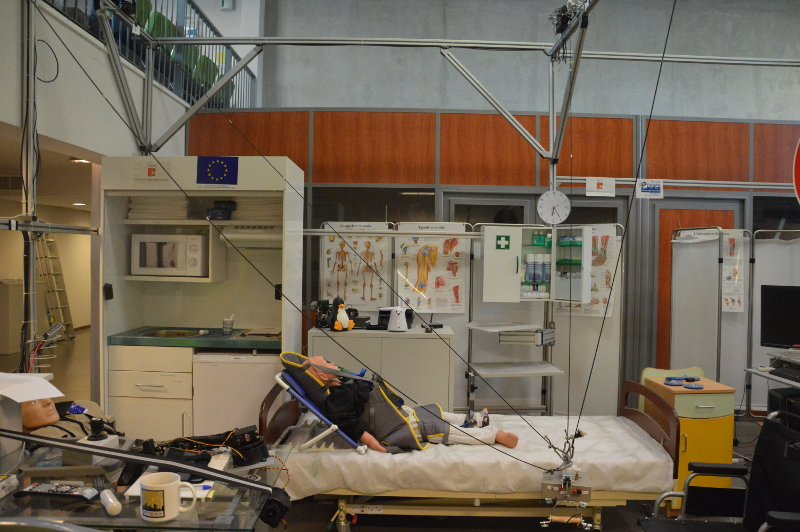
\includegraphics[width=.6\linewidth]{./chapter0/figures/view_appartment01.jpg}} 
\\
  \subfloat[Vue aérienne de l'appartement-témoin]{\label{intro:fig10view1} 
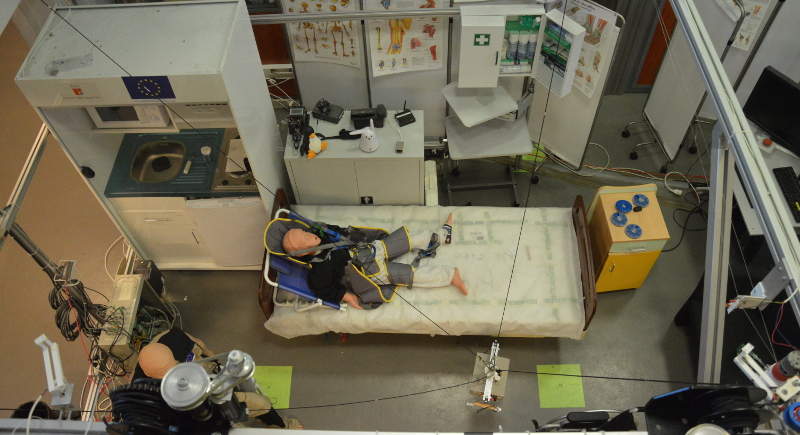
\includegraphics[width=.6\linewidth]{./chapter0/figures/view_appartment04.jpg}} 
\\
  \subfloat[Plateforme de {\tt Marionet-Assist}]{\label{intro:fig10view2}
  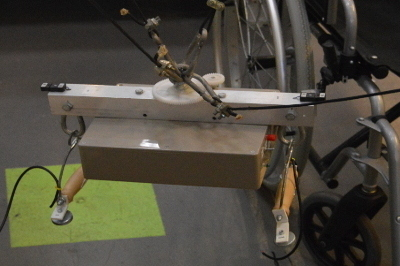
\includegraphics[width=.6\linewidth]{./chapter0/figures/view_plateform.jpg}} 
\\
  \subfloat[Système d'enroulement et actionneurs pour un 
câble]{\label{intro:fig10view3}
  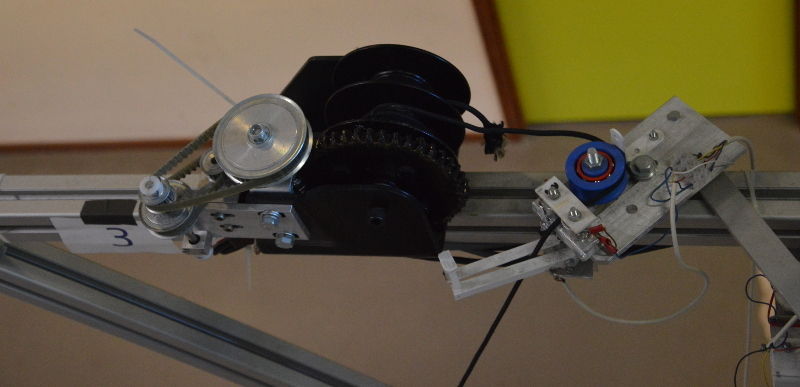
\includegraphics[width=.6\linewidth]{./chapter0/figures/view_winches02.jpg}}
    \caption{\footnotesize{{\tt Marionet-Assist}}}
\label{intro:fig10}
\end{figure}

Ces propriétés font de {\tt Marionet-Assist} un robot adapté au contexte pour 
lequel il a été conçu. Nous avons cependant souhaité améliorer ses 
fonctionnalités de manipulation en lui permettant de ne pas seulement déplacer 
une personne, mais également des objets de la vie quotidienne. Il peut s'agir 
par exemple de ramasser un objet tombé au sol, ou d'amener à l'utilisateur un 
objet (des lunettes par exemple) localisé à un endroit de la pièce éloigné de 
celui auquel il se trouve. Afin de localiser l'objet, puis de guider le robot 
dans son déplacement et dans la manipulation de l'objet cible, une caméra a été 
ajoutée sur la plate-forme, de manière à utiliser des techniques 
d'asservissement visuel. Ce sont ces dernières que nous allons à présent 
introduire, avant d'indiquer d'une part les problématiques posées par leur 
utilisation dans ce contexte particulier, et d'autre part les différentes 
possibilités d'améliorations que cela autorise concernant le contrôle des 
robots parallèles à câbles.

\section{Conclusion}

Apr\`es avoir mis en avant les inconv\'enients des architectures s\'eries pour 
certaines t\^aches, nous avons pr\'esent\'e dans un premier temps les 
architectures parall\`eles. Ces derni\`eres permettent en particulier de 
supporter de plus lourdes charges avec une pr\'ecision accrue, pour une taille 
du disposotif moindre. Les robots parall\`eles pr\'esentent cependant 
l'inconv\'enient d'\'evoluer dans un espace de travail restreint. Pour cette 
raison, l'utilisation de c\^ables a \'et\'e propos\'ee \`a la place de jambes 
rigides. Nous avons donc pr\'esent\'e les principales caract\'eristiques des 
robots parall\`eles \`a c\^ables, et identifi\'e les probl\'ematiques 
qu'entra\^inait le choix d'une telle architecture, au rang desquelles la 
complexit\'e accrue des mod\`eles g\'eom\'etriques et cin\'ematiques, ainsi que 
la difficult\'e \`a g\'erer la nature des tensions (nulles ou strictement 
positives) pour chaque c\^able. Enfin, nous avons introduit les 
sp\'ecificit\'es d'une clase particuli\`ere de manipulateurs \`a c\^ables : les 
robots N-1, dont fait parti le prototype que nous avons utilis\'e dans 
le cadre de ce travail, le robot {\tt Marionet-Assist}. Dans le chapitre 
suivant, nous introduirons les principales notions d'asservissement 
visuel, avant de nous pencher sur les specificit\'es d'une utilisation dans le 
contexte de robots parall\`eles \`a c\^ables. Nous pourrons d\`es lors 
clairement identifier les pistes d'am\'elioration de manipulation que 
association de ces deux technologies permet.

\vfill

\pagebreak

%% AV
%\chapter{Contr\^ole des configurations de c\^ables}

Nous proposons dans ce chapitre une m\'ethode permettant de contr\^oler les
c\^ables qui seront en tension le long d'une trajectoire donn\'ee. Dans une
premi\`ere section, nous expliquerons les circonstances qui nous ont
conduits \`a d\'evelopper une m\'ethode de contr\^ole, puis nous introduirons
les concepts n\'ecessaires \`a son d\'eveloppement. La seconde section de ce
chapitre sera consacr\'ee \`a l'\'elaboration de crit\`eres qui nous serviront
\`a s\'electionner les configurations optimisant la stabilit\'e et la
pr\'ecision d'une trajectoire. Enfin, la troisi\`eme et derni\`ere section de
ce chapitre introduira dans un premier temps l'analyse par intervalle dont nous
nous serons servis afin de garantir notre d\'emarche ; puis nous pr\'esenterons
les principes de l'algorithme d\'evelopp\'e et concluerons par l'exposition des
r\'esultats th\'eoriques qui seront valid\'es dans le chapitre consacr\'e aux
simulations et exp\'eri\-mentations.

\section{Notions introductives}

\subsection{Contexte}

Nous avons vu que l'une des sp\'ecificit\'es des manipulateurs parall\`eles \`a
c\^ables est que -- pour une pose donn\'ee -- l'\'equilibre statique peut
\^etre obtenu sans que l'ensemble des c\^ables soient en tension. De plus, il
est possible que dans certaines configurations, il est impossible pour toute
pose que l'ensemble des c\^ables aient une tension strictement positive : ainsi,
pour une configuration $N-1$, avec $N> 3$ et des c\^ables non-\'elastiques, il
est prouv\'e que 3 c\^ables au maximum auront une tension strictement positive,
les $N-3$ autres \'etant d\'etendus \cite{merlet2012}.

La proc\'edure classique consiste \`a donner aux c\^ables d\'etendus une
longueur $\rho_i$ \'egale \`a la distance $||A_iB_i||$. Or, le r\'esultat
peut-\^etre le plus important ici est donn\'e dans \cite{merlet2014} : bien
qu'il s'agisse d'un travail effectu\'e dans le cas de c\^ables \'elastiques,
les r\'esultats restent valables dans la situation in\'elastique, et montrent
qu'il est impossible en pratique de pr\'evoir les modifications du caract\`ere
strictement positif ou nul de la tension pour l'ensemble des c\^ables lors d'une
trajectoire donn\'ee. Ainsi, une modification infime de la longueur du c\^able
en tension nulle dont nous avons r\'egl\'e la longueur de mani\`ere \`a ce que
$\rho_i = A_iB_i$ pourra changer compl\`etement la nature de la tension dans
les autres c\^ables et surtout modifier la pose de l'organe terminal.

La cons\'equence de ces ph\'enom\`enes m\'ecaniques est double : d'une part
nous pouvons nous retrouver dans des configurations sous-contraintes, nous
perdons alors le contr\^ole d'un ou plusieurs degr\'es de libert\'es et la
trajectoire n'est plus stable ; d'autre part les modifications soudaines des
tensions perturbent les mouvements de la plate-forme et la pr\'ecision du
positionnement est affect\'ee.

En dehors des questions de s\'ecurit\'es soulev\'ees par ces situations, nous
avons plusieurs fois observ\'e que ces changements subits engendraient des
mouvements ind\'esirables au niveau de l'organe terminal. Principalement,
puisque les degr\'es de libert\'es en rotation ne sont pas contraints sur notre
prototype, des mouvements pendulaires ont parfois \'et\'e g\'en\'er\'es,
conduisant \`a la perte de la cible dans l'image, et donc l'\'echec de
l'asservissement.

Il nous a donc paru n\'ecessaire dans un premier temps de mettre en place une
strat\'egie permettant de garantir la stabilit\'e des d\'eplacements et la
pr\'ecision des positionnements toutes les fois o\`u cela \'etait possible, et
de pouvoir identifier les situations pour lesquelles il n'y a d'autre solution
que d'adopter un mode de fonctionnement d\'egrad\'e.

\subsection{Les configurations de c\^ables}

Nous appelons {\it configuration de c\^ables}, ou $CC$, la donn\'ee de
l'ensemble des c\^ables qui sont en tension strictement positive. Ainsi, pour
un robot \`a $n$ c\^ables pour $d$ degr\'es de libert\'e, nous noterons
$CC_{k_1, k_2, \dots k_m}$ la configuration pour laquelle les c\^ables $k_1,
k_2, \dots k_m$ sont en tension strictement positive et -- si $m < n$ --  les
c\^ables $k_{m+1}, \dots k_n$ sont d\'etendus. Si la configuration est telle
qu'elle permet avec les $m$ c\^ables en tension de contr\^oler les $d$ de
degr\'es de libert\'es, nous la noterons $\overline{CC}_{k_1, k_2, \dots k_m}$.

Si l'ensemble $k_1, \dots k_p$ est strictement inclus dans l'ensemble $k_1,
\dots k_m$, on pourra \'ecrire $CC_{k_1, \dots k_p} < CC_{k_1, \dots
k_m}$.

Prenons l'exemple d'un robot $4-1$ dont les c\^ables $0, 1, 2, 3$ sont
dispos\'es de mani\`ere \`a ce qu'aucun triplet $A_iA_jA_k$ de points d'attaches
ne soit align\'e. Les configurations possibles pour un tel robot sont :
$\overline{CC}_{012}, \overline{CC}_{013}, \overline{CC}_{023},
\overline{CC}_{123}$, $CC_{01}, CC_{02}, CC_{03}, CC_{12}, CC_{13}, CC_{23},
CC_{0}, CC_{1}, CC_{2}, CC_{3}$. On notera ici que la configuration
${CC}_{0123}$ n'a pas de sens sur ce robot particulier.

Nous appelons {\it coordonn\'ees situ\'ees} ${}^s{\bf P}$ d'un point
${\bf P}$ la donn\'ee de ses param\`etres de pose ${\bf X}$ et de la
configuration de c\^ables dans laquelle il se trouve :

$${}^s{\bf P} := ({\bf X} ; CC_{k_1, \dots k_m})$$

L'ensemble des points $\bf P$ tels qu'il existe ${}^s {\bf P} :=
({\bf X} ; CC_{k_1, \dots k_m})$ pour $CC_{k_1, \dots k_m}$ fix\'e est appel\'e
l'{\it espace l\'egal} de $CC_{k_1, \dots k_m}$, not\'e $El(CC_{k_1, \dots
k_m})$. Nous noterons de plus $\overline{El}(CC_{k_1, \dots
k_m})$ la fermeture de ${El}(CC_{k_1, \dots k_m})$, \`a savoir l'ensemble :
$$\overline{El}(CC_{k_1, \dots k_m}) := \bigcup
El(CC_{k_1, \dots k_p}), CC_{k_1, \dots k_p} < CC_{k_1, \dots k_m}$$

De la m\^eme mani\`ere, pour un m\^eme point $\bf P$, l'ensemble $Sl$
correspond \`a l'ensemble des configurations de c\^ables $CC_{k_1, \dots k_m}$
telles qu'il existe ${}^s{\bf P} \in El(CC_{k_1, \dots k_m})$. Ici,
$\overline{Sl}$ repr\'esentera l'ensemble des $\overline{CC}_{k_1, \dots k_m}$
pour lesquelles il existe ${}^s{\bf P} \in El(\overline{CC}_{k_1, \dots k_m})$.

Soit maintenant $\mathcal O({\bf S}, {\bf G})$ l'ensemble des points ${\bf
P}_i$ qui constituent une trajectoire allant du point ${\bf S}$ au point ${\bf
G}$. Nous noterons $\mathcal O({\bf S}, {\bf G}) \vartriangleleft
El(CC_{k_1, \dots k_m})$ la situation pour laquelle $\forall {\bf P_i} \in
\mathcal O({\bf S}, {\bf G}), \exists {}^s{\bf P}_i \in El(CC_{k_1, \dots
k_m})$, soit que la trajectoire appartient int\'egralement \`a l'espace l\'egal
de $CC_{k_1, \dots k_m}$.

Lorsque nous n'avons pas cette relation, nous avons besoin de d\'efinir des
r\'egions de transferts. Soit deux configurations de c\^ables
$CC_{k_1, \dots k_m}$ et $CC_{k_1, \dots k_p}$, que pour un instant nous
noterons respectivement $CC_i$ et $CC_j$. Nous d\'efinissons l'ensemble
$\overset{\circ}{Tr_{ij}} = El(CC_i) \cap El(CC_j)$ comme l'ensemble des points
${\bf P}$ pour lesquels il existe ${}^sP_i \in El(CC_i)$ et ${}^sP_j \in
El(CC_j)$. Un changement de coordonn\'ees situ\'ees de ${}^sP_i$ vers ${}^sP_j$
sera dans ce cas appel\'e un {\it transfert simple}. Lorsque
$\overset{\circ}{Tr_{ij}} = \emptyset$, mais qu'il existe, pour un point ${\bf
P}$, ${}^sP_i \in \overline{El}(CC_i)$ et ${}^sP_j \in \overline{El}(CC_j)$, nous
appelerons $\partial Tr_{ij}$ l'ensemble des points de {\it transfert marginal}
entre les configurations $CC_i$ et $CC_j$. L'espace de transfert total $Tr_{ij}$
est alors la r\'eunion des espaces de transferts simple et marginal
correspondants.

Supposons par exemple que ${\bf S} \in El(CC_1)$, ${\bf G} \in El(CC_2)$ et qu'il existe un point ${\bf M}$ tel que $\mathcal O({\bf S}, {\bf M}) \vartriangleleft
El(CC_1)$ et $\mathcal O({\bf M}, {\bf G}) \vartriangleleft El(CC_2)$, alors on pourra écrire $\mathcal O({\bf S}, {\bf G}) \vartriangleleft El(CC_1) \cup \overset{\circ}{Tr_{12}} \cup El(CC_2)$. De la même manière, si un point ${\bf M}$ est tel que $\mathcal O({\bf S}, {\bf M}) \vartriangleleft
\overline{El}(CC_1)$ et $\mathcal O({\bf M}, {\bf G}) \vartriangleleft \overline{El}(CC_2)$, alors nous pourrons écrire $\mathcal O({\bf S}, {\bf G}) \vartriangleleft El(CC_1) \cup \partial Tr_{12} \cup El(CC_2)$. Nous appellerons {\it trajet} l'ensemble des configurations de c\^ables et régions de transferts nécessaires au parcours d'une trajectoire. On distinguera les situations suivantes :
\begin{itemize}
 \item {\it trajet trivial} : l'intégralité de la trajectoire peut être réalisée à partir d'une seule configuration de câbles.
 \item {\it trajet simple} : la trajectoire requiert au moins un transfert ; tous les transferts sont simples.
 \item {\it trajet partiellement marginal} : la trajectoire requiert au moins un transfert ; il existe au moins un transfert simple et un transfert marginal.
 \item {\it trajet marginal} : la trajectoire requiert au moins un transfert ; tous les transferts sont marginaux.
\end{itemize}

Lorsque plusieurs trajets existent, nous essaierons alors de définir des relations d'ordre nous permettant de sélectionner le meilleur trajet possible en fonction d'un ou plusieurs critères préalablement définis : ce sera l'objet de la seconde section de ce chapitre.

\subsection{Robots d\'eriv\'es et robot int\'egral}

Soit un robot $4-3-1$, contrôlé par $4$ câbles dont $3$ (les câbles $i, j, k$) sont attachés au même point ${\bf B}_1$ sur l'organe terminal, et un quatrième (câble $l$) relié à celle-ci en un point ${\bf B}_2 \neq {\bf B}_1$. Il a été montré dans \cite{merlet2013-431} que pour une pose donnée, nous pouvions nous retrouver dans des configurations telles que l'un des câbles $i, j$ ou $k$ est détendu -- auquel cas l'auteur parle de configuration $3-2-1$) -- ou encore le câble $l$ -- il s'agira alors d'une configuration $3-1$). Ces deux situations présentent des différences non négligeables du point de vue des propriétés du robot, tout autant au niveau du contrôle que des différents modèles géométriques et cinématiques. La question se pose alors de savoir s'il est plus pertinent d'adopter une démarche {\it top-down} consistant à rechercher les propriétés du robot $4-3-1$ et les décliner ensuite selon les situations, ou au contraire une démarche {\it bottom-up} qui partirait des propriétés spécifiques à chaque possibilité de configuration pour ensuite construire un fonctionnement global.

Un second argument en faveur de cette interrogation est soulevé dans \cite{merlet2012}. Pour rappel, l'équilibre statique s'exprime par la formule suivante : $\mathcal {\bf F} = {\bf J}^{-T} {\bf \tau}$. Or, afin de déterminer les tensions dans les différents câbles, il faut inverser cette relation. Lorsque la matrice jacobienne n'est pas inversible ({\it a fortiori} lorsqu'elle n'est pas carrée), l'auteur montre que l'utilisation de la matrice pseudo-inverse n'est pas appropriée et donne des résultats qui peuvent être faux. On peut se demander dès lors si l'expression de cette première jacobienne est la plus pertinente, s'il n'existe pas une autre approche de la modélisation du robot qui en permettrait une meilleure intuition et utilisation.

Soit $A^{n, m}$ un manipulateur parall\`ele \`a $m$ c\^ables d\'evelopp\'e pour 
contr\^oler au plus $n$ degr\'es de libert\'es, que nous appellerons {\it 
robot maximal}. Le couple ${n, m}$ repr\'esente la {\it signature} du robot et 
sera ici appel\'ee sa {\it signature maximale}.

Associ\'e à un espace de travail $W$, nous dirons qu'il est
\begin{itemize}
 \item {r\'ealisable} s'il existe une pose dans $W$ telle que l'ensemble des 
c\^ables sont en tension
  \item {\it concr\^et} si pour toute pose de $W$ l'ensemble des c\^ables sont 
en tension
  \item {\it abstrait} si il n'existe aucune pose dans $W$ telle que l'ensemble 
des c\^ables sont en tension
\end{itemize}

Nous d\'efinissons une première op\'eration appel\'ee {\it concr\^etisation} 
consistant pour un robot r\'ealisable \`a lui associer le sous-espace de $W_i 
\subset W$ pour lequel il pourra \^etre dit concr\^et. 

Nous \'etablissons ensuite la liste des sous-configurations de c\^ables 
possibles. Nous appelons alors {\it sous-robot} $A_i$ associ\'e \`a la 
configuration de c\^ables $CC_i$ le robot virtuel d\'efini \`a partir des seuls 
c\^ables correspondant \`a sa configuration de c\^ables. Un tel sous-robot 
pourra \`a son tour \^etre abstrait, r\'ealisable ou concr\^et.

Lorsque pour deux configurations de c\^ables $CC_i$ et $CC_j$ nous avons $CC_i< 
CC_j$, alors le sous-robot $A_i$ associ\'e \`a $CC_i$ sera consid\'er\'e comme 
{\it d\'eriv\'e} de $A_j$. S'il existe un ensemble $CC_\alpha$ et un robot 
$A_j$ associ\'e \`a la configuration de c\^ables $CC_j$ tels que $\forall CC_i 
\in CC_alpha, CC_i < CC_j$ et $\forall CC_k \notin CC_alpha, CC_i \nless 
CC_j$, alors on dira de $A_j$ qu'il est un {\it robot int\'egral} des robots 
associ\'es aux configurations de c\^ables $CC_i \in CC_\alpha$.

Pour chaque robot $A_i$ d\'eriv\'e ou int\'egral, nous pouvons, lorsqu'il est 
r\'ealisable, lui associer son sous-espace concr\^etis\'e $W_i$. Notons que 
si $A_i$ d\'erive de $A_j$, cela ne signifie pas pour autant que $W_i 
\subset W_j$. Nous adjoindrons \'egalement \`a tout robot $A_i$ une signature 
$(p,q)$, $q$ repr\'esentant le nombre de degr\'es de libert\'es qu'il est 
possible de contr\^oler gr\^ace \`a sa configuration de $p$ c\^ables.

Nous partons donc du robot maximal pour en d\'eduire les diff\'erents 
sous-robots possibles. Parmi ceux-ci, nous distinguons ceux qui entretiennent 
des relations de d\'erivation et int\'egration tels que nous les avons 
d\'efinies. Puis il nous faut pour chaque sous-robot \'etudier ses 
propri\'et\'es propres et s'interroger sur la mani\`ere dont elles \'evoluent 
entre robots d\'eriv\'es et int\'egraux. Il doit alors \^etre possible en 
fonction d'une t\^ache prescrite d'obtenir une relation d'ordre entre les 
sous-robots et de choisir celui qui nous semble le plus appropri\'e \`a la 
r\'ealisation de cette t\^ache.

Parmi les propri\'et\'es qui peuvent \^etre d\'eduites par relations de 
d\'erivations et int\'egrations, la d\'etermination de la Jacobienne nous 
int\'eresse particuli\`erement dans le cadre de ce travail. Nous d\'efinissons 
d\`es lors les op\'erateurs suivantes :

\begin{itemize}
 \item {\it d\'erivateur} : soient $A_i$ et $A_j$ tels que le premier d\'erive 
du second, et ${\bf J}^{-1}_i$, ${\bf J}^{-1}_j$ leurs matrices jacobiennes 
inverses respectives ; on appelle {\it d\'erivateur} la matrice ${\bf D}$ telle 
que $ {\bf D} {\bf J}^{-1}_j = {\bf J}^{-1}_i$.
 \item {\it int\'egrateurs} : soit $A_j$ un robot int\'egral des robots 
$A_{i_1}, \dots, A_{i_p}$ ; on appelle {\it int\'egrateurs} les matrices 
${\bf I}_1, \dots {\bf I}_p$ tels que $\sum_{k=1}^p {\bf I}_k {\bf J}^{-1}_k = 
{\bf J}^{-1}_j$, avec ${\bf J}^{-1}_k$ les matrices jacobiennes inverses 
respectives des robots $A_{i_k}$.
\end{itemize}


\subsection{Illustration avec le robot {\tt Marionet-Assist}}

\vskip -100pts

\begin{figure}[!ht]
  \centering
    \def\svgwidth{.65\linewidth}
  \input{./chapter01/figures/CC_41.pdf_tex}
    \caption{\footnotesize{Les diff\'erentes configurations de c\^ables du 
{\tt Marionet-Assist} : les fl\`eches noires repr\'esentent les inclusions et 
les lignes en pointill\'es bleus indiquent une r\'egion de transfert simple.}}
\label{chap01:fig0}
\end{figure}

Equip\'e de $4$ c\^ables reli\'es en un m\^eme point \`a l'organe 
terminal (index\'es dans le sens trigonom\'etrique en partant du coin 
bas-gauche), les diff\'erentes confi\-gurations de c\^ables pouvant \^etre 
obtenues \`a partir de {\tt Marionet-Assist} sont :
\begin{itemize}
 \item $4 CC$ \`a $1$ c\^able : $CC_0, CC_1, CC_2, CC_3$
  \item $6 CC$ \`a $2$ c\^ables : $CC_{01}, CC_{12}, CC_{23}, CC_{30}, CC_{02}, 
CC_{13}$, les deux derni\`eres pr\'esentant la caract\'eristique que 
$El(CC_{02}) \cap El(CC_{13}) \neq \emptyset$ (il existe donc un transfert 
simple \`a 2 degr\'es de libert\'e entre ces deux configurations).
  \item $4 CC$ \`a $3$ c\^ables : $\overline{CC}_{012}, \overline{CC}_{013}, 
\overline{CC}_{023}, \overline{CC}_{123}$. Il existe de plus des r\'egions de 
transferts simples entre plusieurs de ces configurations de c\^ables.
\end{itemize}

Ces relations sont reprises dans la Fig.\ref{chap01:fig0}. Le graphe ainsi 
obtenu permet par exemple de d\'efinir les {\it trajets} possibles pour une 
s\'equence donn\'ee, et de calculer le {\it trajet} optimisant un crit\`ere en 
attribuant les poids correspondants aux noeuds et fl\`eches du graphe. On voit 
par exemple que pour passer de $\overline{CC}_{013}$ \`a $\overline{CC}_{123}$, 
il est possible d'utiliser une {\it transition marginale} via $CC_{13}$, ou 
encore deux trajets \`a une transition simple, l'un passant par 
$\overline{CC}_{012}$ et l'autre par $\overline{CC}_{023}$, ou bien encore 
d'autres combinaisons marginales et partiellement marginales.

Le robot maximal et ses sous-robots sont repr\'esent\'es dans la 
Fig.\ref{chap01:fig1}, ainsi que leurs relations de d\'erivation et 
d'int\'egration. Dans le cas du robot {\tt Marionet-Assist}, le robot maximal 
est abstrait, et il existe $4$ robots r\'ealisables dans $A^{3,3}$, $6$ dans 
$A^{2,2}$ et quatre dans $A^{1,1}$. Pour chacun des robots r\'ealisables, 
l'espace de concr\^etisation correspond \`a l'ouvert obtenu par projection 
verticale des droites reliant les points d'attaches correspondant aux 
configurations de c\^ables associ\'ees. Ainsi, l'espace de concr\^etisation de 
$A^{3,3}_{012}$ est obtenu par projection verticale du triangle issu des 
droites ${\bf A}_0{\bf A}_1$, ${\bf A}_1{\bf A}_2$ et ${\bf A}_0{\bf A}_2$, \`a 
l'exception de la projection verticale de ces m\^emes droites. De la m\^eme 
mani\`ere, l'espace de concr\^etisation du robot $A^{2,2}_{0,1}$ est obtenu par 
projection verticale de la droite ${\bf A}_0{\bf A}_1$, \`a l'exception de la 
projection verticale des points ${\bf A}_0$ et ${\bf A}_1$.

\begin{figure}[htp]
  \centering
    \def\svgwidth{.65\linewidth}
  \input{./chapter01/figures/rbt41.pdf_tex}
    \caption{\footnotesize{Schéma de d\'erivation/int\'egration du robot {\tt 
Marionet-Assist} : s'il existe une fl\^eche allant de $CC_i$ \`a $CC_j$, 
alors $CC_i$ d\'erive de $CC_j$ ; $CC_j$ sera le robot int\'egral de l'ensemble 
des robots $CC_k$ qui en d\'erivent.}}
\label{chap01:fig1}
\end{figure}

Soit ${\bf B}$ le point d'attache des c\^ables \`a la plate-forme, ${\bf 
A}_0$, ${\bf A}_1$, ${\bf A}_2$ et ${\bf A}_3$ les points de sorties 
respectifs des $4$ c\^ables, et $\rho_0$, $\rho_1$, $\rho_2$ et $\rho_3$ les 
longueurs de c\^ables associ\'ees. La jacobienne inverse du robot est donn\'ee 
par la matrice dont les lignes sont les vecteurs $\frac {{\bf A}_i{\bf 
B}}{\rho_i}$. La {\it jacobienne inverse maximale} est donc :
\begin{equation}
{\bf J}^{-1} = 
\begin{bmatrix}
\frac {{\bf A}_{0_x}{\bf B}_x} {\rho_0} & \frac {{\bf A}_{0_y}{\bf B}_y} 
{\rho_0} & \frac {{\bf A}_{0_z}{\bf B}_z} {\rho_0} \\
\frac {{\bf A}_{1_x}{\bf B}_x} {\rho_1} & \frac {{\bf A}_{1_y}{\bf B}_y} 
{\rho_1} & \frac {{\bf A}_{1_z}{\bf B}_z} {\rho_1} \\
\frac {{\bf A}_{2_x}{\bf B}_x} {\rho_2} & \frac {{\bf A}_{2_y}{\bf B}_y} 
{\rho_2} & \frac {{\bf A}_{2_z}{\bf B}_z} {\rho_2} \\
\frac {{\bf A}_{3_x}{\bf B}_x} {\rho_3} & \frac {{\bf A}_{3_y}{\bf B}_y} 
{\rho_3} & \frac {{\bf A}_{3_z}{\bf B}_z} {\rho_3} \\
\end{bmatrix}
\label{chap01:eq01}
\end{equation}

Le d\'erivateur permettant de d\'eduire la jacobienne inverse associ\'ee au 
robot $A^{3,3}_{0, 1, 2}$ \`a partir de la jacobienne inverse maximale 
sera la matrice :
\begin{equation}
{\bf D}_{012/3} = 
\begin{bmatrix}
1 & 0 & 0 & 0\\
0 & 1 & 0 & 0\\
0 & 0 & 1 & 0
\end{bmatrix}
\label{chap01:eq02}
\end{equation}

Le d\'erivateur permettant de d\'eduire la jacobienne inverse du robot 
$A^{2,2}_{0, 1}$ \`a partir de $J^{-1}_{012}$ sera :
\begin{equation}
{\bf D}_{01/2} = 
\begin{bmatrix}
1 & 0 & 0\\
0 & 1 & 0
\end{bmatrix}
\label{chap01:eq03}
\end{equation}

Les int\'egrateurs permettant par exemple de d\'eduire $A^{3,3}_{0, 1, 2}$ \`a 
partir de $A^{2,2}_{0, 1}$, $A^{2,2}_{0, 2}$ et $A^{2,2}_{1,2}$ seront 
respectivement :
\begin{equation}
{\bf I}_{01+2} = 1/2
\begin{bmatrix}
1 & 0 \\
0 & 1 \\
0 & 0
\end{bmatrix}
\quad
{\bf I}_{02+1} = 1/2
\begin{bmatrix}
1 & 0 \\
0 & 0 \\
0 & 1
\end{bmatrix}
\quad
{\bf I}_{12+0} = 1/2
\begin{bmatrix}
0 & 0 \\
1 & 0 \\
0 & 1
\end{bmatrix}
\label{chap01:eq04} \quad
\end{equation}
ce qui nous donne bien ${\bf J}^{-1}_{012} = {\bf I}_{01+2} {\bf J}^{-1}_{01} + 
{\bf I}_{02+1} {\bf J}^{-1}_{02} + {\bf I}_{12+0} {\bf J}^{-1}_{12}$.

Nous prenons d\`es lors le parti de n'accorder une pertinence physique qu'aux 
seules jacobiennes de robots concr\^ets.

Prenons l'exemple d'un robot dont les coordonn\'ees des points d'attaches sont 
${\bf A}_0 = (0.0, 0.0, 1.0)$, ${\bf A}_1 = (1.0, 0.0, 1.0)$, ${\bf A}_2 = 
(1.0, 1.0, 1.0)$ et ${\bf A}_3 = (0.0, 1.0, 1.0)$. Soit ${\bf S} = (0.2, 0.7, 
0.8)$ le point de d\'epart d'une trajectoire et ${\bf G} = (0.8, 0.6, 0.6)$ son 
point d'arriv\'ee. La projection horizontale de ${\bf S}$ appartient aux 
triangles dont les sommets respectifs sont ${\bf A}_0{\bf A}_1{\bf A}_3$ et 
${\bf A}_0{\bf A}_2{\bf A}_3$ ; la projection horizontale de ${\bf G}$ 
appartient quant \`a elle aux triangles dont les sommets respectifs sont ${\bf 
A}_1{\bf A}_2{\bf A}_3$ et ${\bf A}_0{\bf A}_1{\bf A}_2$. Supposons que pour 
${\bf S}$ nous partions de $CC_{013}$. Une premi\`ere solution visible 
dans \ref{chap01:fig0} pourrait \^etre de passer par une transition marginale 
correspondant \`a $CC_{13}$ de mani\`ere \`a continuer avec $CC_{123}$. Une 
autre possibilit\'e consiste \`a se mettre en configuration $CC_{023}$ 
(tranfert simple) puis d'utiliser un transfert simple de $CC_{023}$ vers 
$CC_{123}$. Une troisi\`eme enfin propose un seul transfert simple de 
$CC_{013}$ vers $CC_{012}$, mais ne peut \^etre parcourue en ligne droite. Deux 
questions se posent alors :
\begin{itemize}
 \item \`a quel point de la trajectoire op\'erer le transfert ?
  \item  deux transferts simples valent-ils mieux qu'un seul transfert marginal 
? qu'un seul transfert simple mais dont la trajectoire est plus complexe ? 
\end{itemize}

R\'epondre \`a ces questions n\'ecessite dans un premier temps de 
pouvoir comparer les propri\'et\'es locales des sous-robots associ\'es \`a 
chaque configuration de c\^ables impliqu\'ee, mais surtout de pouvoir 
pond\'erer les configurations et transferts de mani\`ere \`a d\'eterminer le 
trajet optimal. Nous proposons donc dans la suite de ce chapitre d'\'etudier 
plusieurs crit\`eres permettant une optimisation des trajets.

\section{Crit\`eres d'optimisation et d'\'evaluation}

\subsection{Travaux pr\'eliminaires}

Au contraire des CDPR pleinement contraints dont la pose est d\'etermin\'ee par 
les longueurs des c\^ables (quand un nombre suffisant de ceux-ci sont en 
tension), les robots en configuration suspendue utilise la gravit\'e pour 
contraindre la pose. Si ce choix de configuration poss\`ede plusieurs avantage, 
dont celui d'utiliser un nombre inf\'erieur de c\^ables (ce qui r\'eduit par 
exemple les possiblit\'es de collision), il rend cependant le syst\`eme plus 
sensibles aux perturbations, ce qui affecte la qualit\'e du mouvement du robot.

Le choix d'une configuration de c\^ables peut se faire lorsque plusieurs sont 
possibles pour une m\^eme pose. Nous partirons donc du postulat que pour une 
pose ${\bf X}$ il existe un ensemble $CC_\alpha$ de $M$ configurations $CC_{i}$ 
telles que $\forall i \in [1, N], {\bf X} \in El(CC_i)$. Certaines - voire 
toutes - de ces configurations supposent qu'un c\^able au moins est en 
tension nulle.

La strat\'egie g\'en\'eralement utilis\'e dans le contr\^ole des manipulateurs 
parall\`eles \`a c\^ables consiste \`a leur imposer une longueur la plus proche 
possible de la distance ${\bf A}_i{\bf B}$. Or, nous avons \'evoqu\'e \`a 
plusieurs reprises que l'incertitude sur les longueurs ne permettait pas de 
savoir quelle configuration allait succ\'eder au moment $t+1$ \`a celle prise 
effectivement par les c\^ables au moment $t$. Il est donc extr\^emement 
difficile - pour ne pas dire g\'en\'eralement impossible - d'avoir un 
contr\^ole sur les trajets (successions de configurations). Pour autant, 
l'analyse des sous-robots correspondants aux diff\'erentes configurations ne 
manquera pas de r\'ev'eler qu'\`a l'exception de cas rares, les propri\'et\'es 
du manipulateur ne sont pas \'equivalente pour la pose ${\bf X}$.

D\'es lors, plut\^ot que de tenter de garder les longueurs aussi proches 
que possible de leur valeurs th\'eoriques, nous avons propos\'e 
dans \cite{ramadour2014} de forcer la s\'el\'ection d'une configuration en 
ajoutant volontairement aux c\^ables qu'elle suppose mous une longueur 
suppl\'ementaire qui assure -- en fonction de l'incertitude sur les longueurs 
-- qu'il ne changera pas d'\'etat.

La premi\`ere \'etape consiste donc \`a d\'eterminer pour une pose donn\'ee 
l'ensemble des configurations de c\^ables dans lesquelles elle peut se 
retrouver. En hi\'erarchisant ensuite ces configurations \`a partir des 
propri\'et\'es des sous-robots, on en choisit une, puis on ajoute aux 
c\^ables qui n'interviennent pas dans la d\'efinition du sous-robot une 
longueur suppl\'ementaire tant que l'on ne souhaite pas modifier la 
configuration.

L'analyse -- lors d'une trajectoire -- en parall\`ele des propri\'et\'es des 
sous-robots associ\'ees aux configurations possibles permet de d\'eterminer les 
poses pour lesquelles il est souhaitable de changer de configuration. Au point 
de transfert d\'etermin\'e par la comparaison des crit\`eres respectifs, il 
suffit alors de redonner aux c\^ables impliqu\'ees dans la configuration 
post\'erieure leur longueur th\'eorique, et d'ajouter \`a ceux dont on ne veut 
plus se servir une longueur suppl\'ementaire.

Une fa\c con alternative de consid\'erer ce processus consiste \`a envisager 
que nous utilisons une flotte de robots coop\'erants les uns avec les autres 
lors d'une trajectoire. On comprend alors que le transfert d'un robot \`a un 
autre est un moment particulier du contr\^ole. Il implique entre-autres que la 
vitesse du d\'eplacement soit ralentie en ce point particulier de mani\`ere \`a 
minimiser l'influence des perturbations.

Si ce ralentissement peut \^etre consid\'er\'e comme un inconv\'enient, 
il offre toutefois deux avantages majeurs, \`a savoir :
\begin{itemize}
 \item l'existence pour une pose de plusieurs configurations de c\^ables 
possibles devient ici un atout, puisqu'il est permis de choisir celle qui 
optimisera un crit\`ere pr\'e\'etabli, alors que nous ne pouvions 
pr\'ec\'edemment que nous r\'ef\'erer au {\it pire des cas}
  \item en divisant la t\^ache en sous-robots distincts dont nous d\'ecidons 
lequel prend en charge le d\'eroulement d'un partie de la trajectoire, nous 
pouvons am\'eliorer les caract\'eristiques du robot global, d\'es lors que 
celles-ci ne sont plus minor\'ees par la situation la pire sur l'espace de 
travail, mais uniquement sur le minimum parmi les meilleures situations en 
chaque point de l'espace.
\end{itemize}

Nous allons \`a pr\'esent voir successivement comment nous proposons 
d'am\'eliorer la stabilit\'e puis la pr\'ecision du manipulateur.
 

\subsection{Am\'elioration de la stabilit\'e}

Am\'eliorer la stabilit\'e est primordial pour deux raisons :
\begin{itemize}
 \item lorsque le manipulateur est utilis\'e dans son contexte originel d'aide 
au d\'eplacement des personnes, cela permet d'une part d'assurer la 
s\'ecurit\'e du processus, en \'evitant la perte de contr\^ole d'un ou 
plusieurs degr\'es de libert\'e, d'autre part l'aisance de l'utilisation en 
n\'egociant les changements de configurations de c\^ables de mani\`ere souple
\item lors d'une op\'eration impliquant un asservissement visuel avec cam\'era 
embarqu\'ee, la moindre perturbation modifie la situation du r\'ef\'erentiel 
cam\'era par rapport au r\'ef\'erentiel de l'organe terminal. D\'es lors, la 
conversion des mesures effectu\'ees sur l'image en commande pour le 
manipulateur est fauss\'ee et l'asservissement \'echoue. Une perturbation trop 
forte peut \'egalement faire sortir la cible de l'image, ce qui conduit 
fatalement \`a l'impossiblit\'e de poursuivre l'utilisation de l'asservissement 
visuel.
\end{itemize} 


\subsubsection{Minimiser la tension}

Pour deux configurations donn\'ees, les tensions exerc\'ees sur les c\^ables de 
chacune d'entre elles diff\`ereront.

Prenons l'exemple du robot $4-1$ dont les points d'attache sont r\'epartis aux 
quatre coins les plus hauts d'un cube d'un m\`etre de c\^ot\'e. Fixons un point 
${\bf B}$ de coordonn\'ees $(0.20, 0.30, 0.80)^T$ (Fig.\ref{chap01:fig3}).

En ce point, deux configurations de c\^ables sont possibles : 
$\overline{CC}_{013}$(Fig.\ref{chap01:fig3view0}) et $\overline{CC}_{023}$(Fig.\ref{chap01:fig3view1}). Ces deux configurations 
permettent de contr\^oler les trois degr\'es de libert\'es en translation.

\begin{figure}[htp]
  \centering
 \subfloat[Le robot en configuration de câbles $\overline{CC}_{013}$]{\label{chap01:fig3view0}
 \def\svgwidth{.45\linewidth}
 \input{./chapter01/figures/tension02.pdf_tex}} \hfill
 \subfloat[Le robot en configuration de câbles $\overline{CC}_{023}$]{\label{chap01:fig3view1}
 \def\svgwidth{.45\linewidth}
 \input{./chapter01/figures/tension01.pdf_tex}} 
    \caption{\footnotesize{Les deux configurations de c\^ables possibles pour 
une pose ${\bf B} = (0.2, 0.3, 0.8)^T$}}
\label{chap01:fig3}
\end{figure}

Les jacobiennes inverses respectives sont :

\begin{equation}
{\bf J}^{-1}_{013} = 
\begin{bmatrix}
0.4851 & 0.7276 & -0.4851 \\
-0.9117 & 0.3419 & -0.2279 \\
0.2649 & -0.9272 & -0.2649
\end{bmatrix},
{\bf J}^{-1}_{023}
\begin{bmatrix}
0.4851 & 0.7276 & -0.4851 \\
-0.7396 & -0.6472 & -0.1849 \\
0.2649 & -0.9272 & -0.2649
\end{bmatrix}
\label{chap01:eq05}
\end{equation}

En posant $m = 1/g$, nous avons ${\boldmath {\mathcal F}} = (0, 0, -1)^T$, ce qui 
nous donne :

\begin{equation}
{\bf \tau}_{013} = 
\begin{bmatrix}
1.0308
0.8775  
1.1325
\end{bmatrix},
\quad
{\bf \tau}_{023}
\begin{bmatrix}
1.4431 \\
1.0817 \\
0.3775
\end{bmatrix}
\label{chap01:eq06}
\end{equation}

Nous pouvons d\'ej\`a v\'erifier qu'un passage non-contr\^ol\'e d'une 
configuration \`a l'autre produit des variations de tensions discontinues, 
alors m\^eme que les deux configurations ont en commun deux c\^ables sur trois.

De plus, la variance des tensions est plus importante pour la 
configuration $\overline{CC}_{023}$, ce qui dénote une répartition in\'egale des efforts sur les câbles.

Nous proposons donc de consid\'erer la norme des tensions th\'eoriques 
obtenues comme critère, et de choisir la configuration qui offre ainsi une meilleure 
r\'epartition, soit dans ce cas $\overline{CC}_{023}$.

Ainsi, en chaque pose, nous calculons pour toutes les configurations de câbles $\overline{CC}_i$ correspondant à une situation d'équilibre statique la mesure $\mathcal M_{\hbox{stab}_i}$ :

\begin{equation}
\mathcal M_{\hbox{stab}_i} = ||{\bf J}_i {\boldmath {\mathcal F}}||
\label{chap01:eq07}
\end{equation}

Posons à présent ${\bf B} = (0.3,0.3,0.3)^T$. Dans ce cas, les deux configurations de câbles possibles sont $\overline{CC}_{013}$ et $CC_{02}$.

Les jacobiennes inverses correspondantes sont :

\begin{equation}
{\bf J}^{-1}_{013} = 
\begin{bmatrix}
0.3665 & 0.3665 & -0.8552 \\  
-0.6767 & 0.2900 & -0.6767 \\  
0.2900 & -0.6767 & -0.6767
\end{bmatrix},
{\bf J}^{-1}_{02}
\begin{bmatrix}
0.3665 & 0.3665 & -0.8552 \\  
-0.5774 & -0.5774 & -0.5774
\end{bmatrix}
\label{chap01:eq08}
\end{equation}

En utilisant pour $A^{2,2}_{02}$ le sous-robot associé à la configuration de câbles $CC_{01}$ la pseudo-inverse de Moore-Penrose pour calculer les tensions théoriques correspondantes, nous obtenons :

\begin{equation}
{\bf \tau}_{013} = 
\begin{bmatrix}
0.4677 \\
0.4433 \\
0.4433
\end{bmatrix},
\quad
{\bf \tau}_{02}
\begin{bmatrix}
0.8185 \\ 
0.5196 
\end{bmatrix}
\label{chap01:eq09}
\end{equation}

Les mesures respectives sont $\mathcal M_{\hbox {stab}_{013}} = 0.7822$ et $\mathcal M_{\hbox {stab}_{02}} = 0.9695$, soit une sélection de la configuration $\overline{CC}_{013}$.

Toutes ces mesures pouvant être réalisées en amont, elles n'impactent pas le temps de calcul de la commande. Ainsi, pour notre robot $4-1$ cubique, pour une valeur de $Z = 0.5$ fixée, les figures \ref{} et \ref{} nous montrent respectivement quelle configuration de câbles sera privilégiée en tout point de l'espace de travail, et l'évolution du critère sur l'ensemble de celui-ci.

\subsubsection{Illustration}

\subsection{Am\'elioration de la pr\'ecision}


\subsubsection{Crit\`eres}

\subsubsection{Illustration}

\section{Algorithme de s\'election de configurations de c\^ables}


\subsection{L'analyse par intervalles}

\subsection{Algorithme}

\subsection{R\'esultats th\'eoriques}


%\pagebreak

%% AV CDPR
\chapter{Asservissement visuel des robots à c\^ables}

Les manipulateurs parallèles à câbles peuvent s'avérer un choix pertinent d'architecture dès lors que tâche requiert tout ou partie des propriétés suivantes :
\begin{itemize}
 \item pouvoir être effectuée dans un large espace de travail
 \item pouvoir manipuler des charges importantes
 \item pouvoir être déployée rapidement
 \item garantir une précision et une dynamique suffisantes
\end{itemize}

Toutefois, nous avons vu que le contrôle de tels robots posait plusieurs problèmes, parmi lesquels :
\begin{itemize}
 \item des modèles géométriques et cinématiques plus complexes que pour les robots séries
 \item un câble ne pouvant exercer qu'une force unilatérale, il est possible qu'il se retrouve avec une tension nulle ; cela peut donner lieu à des changements discontinus des valeurs de tension pour chaque c\^able, voire la perte d'un ou plusieurs degrés de liberté
 \item des incertitudes mécaniques, particulièrement sur la longueur réelle de déploiement d'un c\^able si nous utilisons un moteur rotatif comme actionneur (le diamètre d'enroulement n'étant alors qu'une approximation).
\end{itemize}

Pour ces raisons, la précision d'une pose dépendra à la fois de son histoire (selon la trajectoire qui y a conduit et l'ensemble des câbles qui auront contribué à son obtention, le positionnement final pourra différer) et de sa robustesse aux incertitudes mécaniques, méthodologiques (simplification des modèles d'élasticité et de pesance des câbles par exemple) et de la précision des calculs.

L'asservissement visuel a donc été proposée à plusieurs reprises afin de résoudre tout ou partie de ces inconvénients. Les stratégies suivantes ont par exemple été mises en place :
\begin{itemize}
 \item une caméra déportée filme l'organe terminal, et par un asservissement en position, entreprend de corriger les erreurs de pose de celui-ci. Sont requis ici que la scène soit dégagée, que la caméra ait un champs de vision suffisamment grand pour pouvoir appréhender l'ensemble de l'espace de travail. Pour autant, une telle méthode ne permet pas de gérer les questions de tensions positives ou nulles dans les câbles.
 \item plusieurs caméras sont utilisées pour filmer les départs des câbles. En utilisant la géométrie plückerienne, ceci permet d'obtenir une estimation précise de la Jacobienne inverse. Pour autant, la question de la répartition des forces dans les câbles n'est là non plus pas considérée. Une telle stratégie suppose que tous les câbles soient en tension, ce qui est par exemple dans certaines architectures impossible, et peut donc conduire à une commande erronée. 
\end{itemize}

Pour autant, utilisées ensemble, ces deux stratégies devraient pouvoir permettre d'assurer la manipulation dans la plupart des cas, sans pour autant le garantir.

Notre objectif ici est donc double : construire dans un premier temps une loi de commande qui soit aussi indépendante que possible des paramètres de pose et des coordonnées articulaires, contrôler dans un deuxième temps les câbles qui seront en tension pour une trajectoire donnée. En effet, dès lors que nous connaissons les câbles qui sont en tension, nous obtenons le rang de la Jacobienne correspondante. Nous pouvons ainsi affiner la commande en cessant de considérer le robot global, pour ne plus prendre en compte que la partie correspondant réellement aux câbles qui agissent sur le déplacement. Nous utiliserons alors ce que nous définirons plus tard comme étant la {\it Jacobienne du sous-robot associe à une configuration de câbles}. L'utilisation d'une loi de commande articulaire exploitant des informations visuelles adaptées permettra de s'abstraire lors d'une commande cinématique à la fois des incertitudes liées à la commande du robot, mais également aux problèmes soulevés dans le chapitre précédent concernant l'estimation de la matrice d'interaction.

Ce chapitre est consacré à l'élaboration d'une telle loi de commande. Pour cela, nous présenterons dans un premier temps les spécificités d'un asservissement visuel classique de robots parallèles à câbles. Dans une seconde section, nous montrerons dans quelle mesure nous pouvons y trouver des améliorations concernant la précision du manipulateur et la robustesse aux erreurs et incertitudes diverses. La troisième section développera les conditions d'une loi de commande articulaire reposant sur une première estimation de la matrice d'interaction articulaire et un schéma itératif assurant la convergence vers une trajectoire linéaire. Enfin, une quatrième section présentera les conclusions de ce premier volet de notre étude. L'ensemble des simulations et validations expérimentales se trouveront dans le chapitre final.

\section{Elaboration d'un asservissement visuel des robots à c\^ables}

Cette première section est consacrée à l'élaboration d'une loi de commande classique adaptée aux robots parallèles à câbles. Ceci nous permettra de montrer les améliorations apportées par l'asservissement visuel (seconde section du chapitre) et servira de support de comparaison pour la loi simplifiée qui sera élaborée en troisième section.

\subsection{Construction de la loi de commande classique}






\subsection{Utilisation des moments 2D}

\subsection{Cas du robot N-1}

\section{Amélioration de la robustesse et de la précision}

\subsection{Robustesse aux incertitudes de modèle}

\subsection{Amélioration de la précision}

\subsection{Illustration des limites avec le cas N-1}


\section{Asservissement simplifié : commande articulaire}

\subsection{Motivations}

\subsection{Le schéma de Broyden}

\subsection{Commande simplifiée}

\subsection{Cas N-1}

\section{Conclusions}

%\pagebreak

%% CC
%\chapter{Contr\^ole des configurations de c\^ables}

Nous proposons dans ce chapitre une m\'ethode permettant de contr\^oler les
c\^ables qui seront en tension le long d'une trajectoire donn\'ee. Dans une
premi\`ere section, nous expliquerons les motivations qui nous ont
conduits \`a d\'evelopper une telle m\'ethode de contr\^ole, puis 
nous introduirons les concepts n\'ecessaires \`a son d\'eveloppement. La 
seconde section de ce chapitre est consacr\'ee \`a l'\'elaboration de 
crit\`eres qui nous serviront \`a s\'electionner les configurations optimisant 
la stabilit\'e et la pr\'ecision d'une trajectoire. Enfin, la troisi\`eme et 
derni\`ere section de ce chapitre introduira dans un premier temps l'analyse 
par intervalle dont nous nous sommes servis afin de garantir notre d\'emarche ; 
puis nous pr\'esenterons les principes de l'algorithme d\'evelopp\'e et 
concluerons par l'exposition des r\'esultats th\'eoriques qui seront valid\'es 
dans le chapitre consacr\'e aux simulations et exp\'eri\-mentations.

\section{Notions introductives}

\subsection{Contexte}

Nous avons vu que l'une des sp\'ecificit\'es des manipulateurs parall\`eles \`a
c\^ables est que -- pour une pose donn\'ee -- l'\'equilibre statique peut
\^etre obtenu sans que l'ensemble des c\^ables soient en tension. De plus, il
arrive dans certains cas qu'il soit impossible, quelle que soit la pose du 
robot, que l'ensemble des c\^ables aient une tension strictement positive : 
ainsi, pour une configuration N-1 ($N$ câbles distincts reliés en un seul point 
${\bf B}$ à la plateforme), avec $N> 3$ et des c\^ables non-\'elastiques, il
est prouv\'e que 3 c\^ables au maximum auront une tension strictement positive,
les $N-3$ autres \'etant d\'etendus \cite{merlet2012}.

Pour l'ensemble des contrôleurs proposés dans la littérature, ce phénomène est 
ignoré : soit le contrôle est positionnel, auquel cas les $\rho_i$ sont ajustés 
sur la distance $||{\bf A}_i {\bf B}||$, soit il s'agit d'un contrôle en force 
sans trop se soucier de savoir si toutes les tensions sont commandables, soit 
éventuellement un contrôleur hybride/position sous les mêmes hypothèses 
\cite{taghirad2011}, \cite{bedoustani2010}, \cite{weijung2000}, 
\cite{hassan2007}, \cite{arsenault2010}, \cite{lenarcic2002}. Or, le r\'esultat 
peut-\^etre le plus important ici est donn\'e dans \cite{merlet2014check}, 
l'auteur montrant qu'il est impossible en pratique de pr\'evoir les 
modifications du caract\`ere strictement positif ou nul de la tension pour 
l'ensemble des c\^ables lors d'une trajectoire donn\'ee. Ainsi, une modification 
infime de la longueur du c\^able en tension nulle dont nous avons r\'egl\'e la 
longueur de mani\`ere \`a ce que $\rho_i = A_iB_i$ pourra changer compl\`etement 
la nature de la tension dans les autres c\^ables et surtout modifier la pose de 
l'organe terminal.

La cons\'equence de ces ph\'enom\`enes m\'ecaniques est double : d'une part
nous pouvons nous retrouver dans des configurations sous-contraintes, nous
perdons alors le contr\^ole d'un ou plusieurs degr\'es de libert\'es et la
trajectoire n'est plus stable ; d'autre part les modifications soudaines des
tensions perturbent les mouvements de la plate-forme et la pr\'ecision du
positionnement est affect\'ee.

Dans le cas du robot $4-1$, la figure \ref{chap03:fig0000} permet de 
comprendre pourquoi l'équilibre statique n'est possible avec trois câbles en 
tension que si le point ${\bf B}$ correspondant à la pose de la plate-forme 
appartient à la projection verticale du triangle formé par les points de sortie 
des trois câbles. En effet, si ce n'est pas le cas, que le point est en dehors 
du triangle, on voit bien que les forces ne s'opposent pas dans au moins une 
direction, rompant ainsi l'équilibre statique.

\begin{figure}[!ht]
  \centering
    \def\svgwidth{.65\linewidth}
  \input{./chapter03/figures/configonly3.pdf_tex}
    \caption{\footnotesize{En haut \`a gauche, la pose initiale avec les 
c\^ables 1, 2 et 3 en tension. En haut \`a droite, la diminution de la 
longueur $\rho_3$ implique va d\'acer la masse autour de l'axe ${\bf 
A}_i{\bf A}_j$, ce qui a pour effet de modifier la pose. En bas \`a gauche, le 
d\'eplacement du point $\bf B$ modifie les distances $||{\bf A}_i{\bf B}||$. En 
particulier, nous avons ici $\rho_j > ||{\bf A}_j{\bf B}||$, et donc le c\^able 
devient mou. En bas \`a droite, nouvelle pose, avec les c\^ables $i, k$ et $3$ 
en tension.}}
\label{chap03:fig0001}
\end{figure}

La démonstration de l'impossibilité d'avoir plus de $3$ câbles en tension 
simultanée repose également sur l'équilibre statique. Dans \cite{merlet2012}, 
ceci est démontré pour toute configuration à $N > 3$ câbles. Le cas à quatre 
câbles est relativement simple et peut être exposé ainsi (cf. 
Fig. \ref{chap03:fig0001}) :
\begin{enumerate}
 \item soit ${\bf B}$ une pose atteinte \`a l'aide des c\^ables $0,1,2$, pour 
laquelle nous avons l'\'equilibre statique. Alors la projection de ${\bf B}$ 
sur le plan auxquels les ${\bf A}_i$ appartiennent se trouve dans le triangle 
form\'e par les trois points de sortie ${\bf A}_0, {\bf A}_1, {\bf A}_2$.
\item il existe $(i,j) \in [0,2]$ tels que la droite ${\bf A}_i{\bf A}_j$ 
s\'epare le plan en deux demi-plans : le sous-espace $\mathcal V$ contient le 
troisi\`eme point de sortie ${\bf A}_k$ ainsi que le point ${\bf B}$, tandis 
que le demi-plan $\mathcal V_3$ contient le point ${\bf A}_3$.
\item on suppose que $\rho_3 = ||{\bf A}_3{\bf B}$. Alors une diminution de la 
longueur $\rho_3$ va g\'en\'erer un moment autour de la droite ${\bf A}_i{\bf 
A}_j$. D\`es lors, la distance $||{\bf A}_k{\bf B}||$ va cro\^itre, ce qui 
implique une modification de la pose. Lors de cette modification, nous aurons 
soit $\rho_i > ||{\bf A}_i{\bf B}||$, soit $\rho_j > ||{\bf A}_j{\bf B}||$, ce 
qui aura pour cons\'equence de rendre mous le c\^able concern\'e et conduira 
\`a une pose avec \`a nouveau trois c\^ables en tension, dont ${\bf A}_k$ et 
${\bf A}_3$.
\end{enumerate}

\begin{figure}[!ht]
  \centering
    \def\svgwidth{.65\linewidth}
  \input{./chapter03/figures/ws__out.pdf_tex}
    \caption{\footnotesize{Lorsque le point sort des limites du triangle généré 
par les droites reliant les sorties de câbles, les tensions ne sont plus en 
opposition dans toutes les directions : l'équilibre statique ne peut dès lors 
être maintenu.}}
\label{chap03:fig0000}
\end{figure}

Il existe donc pour un robot $4-1$ quatre ensembles distincts de 3 câbles en 
tension strictement positives, et dans aucune de ces situations les trois 
câbles ne permettent d'atteindre l'intégralité de l'espace de travail en 
maintenant l'équilibre statique.

A titre d'exemple, la figure \ref{chap03:fig000} montre qu'il existe des 
trajectoires qui peuvent être effectuées sans que l'on n'ait besoin de changer 
la nature de la tension dans les câbles, mais qu'il en existe également pour 
lesquelles nous n'aurons d'autres choix que de modifier les câbles en tension. 
Dans cet exemple, le point ${\bf P}_1$ peut soit utiliser les câbles 0, 1, et 3, 
soit les câbles 0, 2, et 3. Le point ${\bf P}_2$ peut être atteint quant à lui 
en utilisant les câbles 0, 2, 3 et 1, 2, 3. On voit alors que nous pouvons 
aller de ${\bf P}_1$ à ${\bf P}_2$ en utilisant uniquement les câbles 0, 2 et 3. 
Si nous étions par contre partis de ${\bf P}_1$, avec les câbles 0, 1 et 3 en 
tension, nous aurions d\^u changer. Le point ${\bf P}_3$ correspond aux 
situations pour lesquelles les câbles 0, 1, 2 ou 1, 2, 3 peuvent être utilisés. 
Il est donc possible d'aller de ${\bf P}_2$ à ${\bf P}_3$ avec les seuls câbles 
1, 2 et 3, mais il n'y a par contre aucune possibilité d'aller de ${\bf P}_1$ à 
${\bf P}_3$ sans changer la nature de la tension des câbles.


\begin{figure}[!ht]
  \centering
    \def\svgwidth{.65\linewidth}
  \input{./chapter03/figures/traj_N1.pdf_tex}
    \caption{\footnotesize{Exemples de trajectoires réalisables avec une seule 
configuration de câbles (lignes bleues pleines) et nécessitant un changement de 
configuration de câbles (ligne rouge en pointillés)}}
\label{chap03:fig000}
\end{figure}

Les comportements décrits correspondent toutefois à une situation idéale. Dans 
les faits, l'utilisation d'un contrôleur discret basé sur une loi de commande 
voulant imposer une valeur $\rho_i = ||{\bf A}_i{\bf B}||$ ne permet pas de 
prédire ce qui se déroulera durant la période d'échantillonnage, durant laquelle 
le système est libre et n'obéit qu'à ses propres lois mécaniques.

\begin{figure}[!htp]
  \centering
    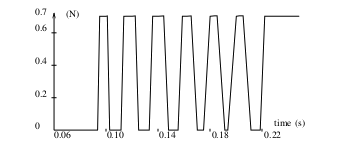
\includegraphics[width=.75\linewidth]{./chapter03/figures/controleur_discret.png}
    \caption{\footnotesize Comportement des tensions dans un câble pour une 
durée d'échantillonnage de $0.2$ secondes}
\label{chap03:fig00}
\end{figure}

La figure \ref{chap03:fig00} montre ce qu'il se passe durant la période 
d'échantillonnage de $0.2$ secondes d'un contrôleur discret. Si la trajectoire 
était parfaitement suivie, nous devrions avoir une valeur te $\tau_n$ nulle sur 
l'ensemble de la période. Or, la trajectoire réelle ne suit pas eaxctement la 
trajectoire théorique. Dès lors, même avec des mesures de longueurs parfaites,le 
système passe immanquablement de poses pour lesquelles la tension est nulle à 
des poses pour lesquelles la tension devient strictement positive. Il faut alors 
en tier les conclusions suivantes :
\begin{itemize}
 \item si $\tau_n \neq 0$ alors qu'il devait être nul, les valeurs des autres 
tensions sont différentes des prédictions 
  \item les câbles étant soumis à des 
alternances entre tension nulle et tension positive, ils s'usent plus rapidement
 \item les variabilités de tensions affectent la précision du manipulateur 
; l'erreur reste cependant assez faible.
 \item un contrôleur en tension ne prenant pas en compte ces propriétés ne peut 
pas vraiment fonctionner.
\end{itemize}

Nous avons de plus plusieurs fois constat\'e que ces changements subits engendraient des
mouvements ind\'esirables au niveau de l'organe terminal. Principalement,
puisque les degr\'es de libert\'es en rotation ne sont pas contraints sur notre
prototype, des mouvements pendulaires ont parfois \'et\'e g\'en\'er\'es,
conduisant \`a la perte de la cible dans l'image, et donc l'\'echec de
l'asservissement.

Il nous a donc paru n\'ecessaire dans un premier temps de mettre en place une
strat\'egie permettant de garantir la stabilit\'e des d\'eplacements et la
pr\'ecision des positionnements toutes les fois o\`u cela \'etait possible, et
de pouvoir identifier les situations pour lesquelles il n'y a d'autre solution
que d'adopter un mode de fonctionnement d\'egrad\'e.

\subsection{Les configurations de c\^ables}

Nous appelons {\it configuration de c\^ables}, ou $CC$, la donn\'ee de
l'ensemble des c\^ables qui sont en tension strictement positive. Ainsi, pour
un robot \`a $n$ c\^ables pour $d$ degr\'es de libert\'e, nous noterons
$CC_{k_1, k_2, \dots k_m}$ la configuration pour laquelle les c\^ables $k_1,
k_2, \dots k_m$ sont en tension strictement positive et -- si $m < n$ --  les
c\^ables $k_{m+1}, \dots k_n$ sont d\'etendus. Si la configuration est telle
qu'elle permet avec les $m$ c\^ables en tension de contr\^oler les $d$ de
degr\'es de libert\'es, nous la noterons $\overline{CC}_{k_1, k_2, \dots k_m}$.

Si l'ensemble $k_1, \dots k_p$ est strictement inclus dans l'ensemble $k_1,
\dots k_m$, on pourra \'ecrire $CC_{k_1, \dots k_p} < CC_{k_1, \dots
k_m}$.

Prenons l'exemple d'un robot $4-1$ dont les c\^ables $0, 1, 2, 3$ sont
dispos\'es de mani\`ere \`a ce qu'aucun triplet $A_iA_jA_k$ de points d'attaches
ne soit align\'e. Les configurations possibles pour un tel robot sont :
$\overline{CC}_{012}, \overline{CC}_{013}, \overline{CC}_{023},
\overline{CC}_{123}$, $CC_{01}, CC_{02}, CC_{03}, CC_{12}, CC_{13}, CC_{23},
CC_{0}, CC_{1}, CC_{2}, CC_{3}$. On notera ici que la configuration
${CC}_{0123}$ n'a pas de sens sur ce robot particulier.

Nous appelons {\it coordonn\'ees situ\'ees} ${}^s{\bf P}$ d'un point
${\bf P}$ la donn\'ee de ses param\`etres de pose ${\bf X}$ et de la
configuration de c\^ables dans laquelle il se trouve :

$${}^s{\bf P} := ({\bf X} ; CC_{k_1, \dots k_m})$$

L'ensemble des points $\bf P$ tels qu'il existe ${}^s {\bf P} :=
({\bf X} ; CC_{k_1, \dots k_m})$ pour $CC_{k_1, \dots k_m}$ fix\'e est appel\'e
l'{\it espace l\'egal} de $CC_{k_1, \dots k_m}$, not\'e $El(CC_{k_1, \dots
k_m})$. Nous noterons de plus $\overline{El}(CC_{k_1, \dots
k_m})$ la fermeture de ${El}(CC_{k_1, \dots k_m})$, \`a savoir l'ensemble :
$$\overline{El}(CC_{k_1, \dots k_m}) := \bigcup
El(CC_{k_1, \dots k_p}), \quad CC_{k_1, \dots k_p} < CC_{k_1, \dots k_m}$$

De la m\^eme mani\`ere, pour un m\^eme point $\bf P$, l'ensemble $Sl$
correspond \`a l'ensemble des configurations de c\^ables $CC_{k_1, \dots k_m}$
telles qu'il existe ${}^s{\bf P} \in El(CC_{k_1, \dots k_m})$. Ici,
$\overline{Sl}$ repr\'esentera l'ensemble des $\overline{CC}_{k_1, \dots k_m}$
pour lesquelles il existe ${}^s{\bf P} \in El(\overline{CC}_{k_1, \dots k_m})$.

Soit maintenant $\mathcal O({\bf S}, {\bf G})$ l'ensemble des points ${\bf
P}_i$ qui constituent une trajectoire allant du point ${\bf S}$ au point ${\bf
G}$. Nous noterons $\mathcal O({\bf S}, {\bf G}) \vartriangleleft
El(CC_{k_1, \dots k_m})$ la situation pour laquelle $\forall {\bf P_i} \in
\mathcal O({\bf S}, {\bf G}), \exists {}^s{\bf P}_i \in El(CC_{k_1, \dots
k_m})$, soit que la trajectoire appartient int\'egralement \`a l'espace l\'egal
de $CC_{k_1, \dots k_m}$.

Lorsque nous n'avons pas cette relation, nous avons besoin de d\'efinir des
r\'egions de transferts. Soit deux configurations de c\^ables
$CC_{k_1, \dots k_m}$ et $CC_{l_1, \dots l_p}$, que pour un instant nous
noterons respectivement $CC_i$ et $CC_j$. Nous d\'efinissons l'ensemble
$\overset{\circ}{Tr_{ij}} = El(CC_i) \cap El(CC_j)$ comme l'ensemble des points
${\bf P}$ pour lesquels il existe ${}^sP_i \in El(CC_i)$ et ${}^sP_j \in
El(CC_j)$. Un changement de coordonn\'ees situ\'ees de ${}^sP_i$ vers ${}^sP_j$
sera dans ce cas appel\'e un {\it transfert simple}. Lorsque
$\overset{\circ}{Tr_{ij}} = \emptyset$, mais qu'il existe, pour un point ${\bf
P}$, ${}^sP_i \in \overline{El}(CC_i)$ et ${}^sP_j \in \overline{El}(CC_j)$, nous
appelerons $\partial Tr_{ij}$ l'ensemble des points de {\it transfert marginal}
entre les configurations $CC_i$ et $CC_j$. L'espace de transfert total $Tr_{ij}$
est alors la r\'eunion des espaces de transferts simple et marginal
correspondants.

Supposons par exemple que ${\bf S} \in El(CC_1)$, ${\bf G} \in El(CC_2)$ et 
qu'il existe un point ${\bf M}$ tel que $\mathcal O({\bf S}, {\bf 
M}) \vartriangleleft El(CC_1)$ et $\mathcal O({\bf M}, {\bf G}) 
\vartriangleleft El(CC_2)$, alors on pourra écrire $\mathcal O({\bf S}, {\bf G}) 
\vartriangleleft El(CC_1) \cup \overset{\circ}{Tr_{12}} \cup El(CC_2)$. De la 
 même manière, si un point ${\bf M}$ est tel que $\mathcal O({\bf S}, {\bf M}) 
\vartriangleleft \overline{El}(CC_1)$ et $\mathcal O({\bf M}, {\bf G}) 
\vartriangleleft \overline{El}(CC_2)$, alors nous pourrons écrire $\mathcal 
O({\bf S}, {\bf G}) \vartriangleleft El(CC_1) \cup \partial Tr_{12} \cup 
El(CC_2)$. Nous appellerons {\it trajet} l'ensemble des configurations de 
c\^ables et régions de transferts nécessaires au parcours d'une trajectoire. On 
distinguera les situations suivantes :
\begin{itemize}
 \item {\it trajet trivial} : l'intégralité de la trajectoire peut être 
réalisée à partir d'une seule configuration de câbles.
 \item {\it trajet simple} : la trajectoire requiert au moins un transfert ; 
tous les transferts sont simples.
 \item {\it trajet partiellement marginal} : la trajectoire requiert au moins 
un transfert ; il existe au moins un transfert simple et un transfert marginal.
 \item {\it trajet marginal} : la trajectoire requiert au moins un transfert 
; tous les transferts sont marginaux.
\end{itemize}

Lorsque plusieurs trajets existent, nous essaierons alors de définir 
des relations d'ordre nous permettant de sélectionner le meilleur trajet 
possible en fonction d'un ou plusieurs critères préalablement définis : ce sera 
l'objet de la seconde section de ce chapitre.

\subsection{Robots d\'eriv\'es et robot int\'egral}

Soit un robot $4-3-1$, contrôlé par $4$ câbles dont $3$ (les câbles $i, j, k$) 
sont attachés au même point ${\bf B}_1$ sur l'organe terminal, et un quatrième 
(câble $l$) relié à celle-ci en un point ${\bf B}_2 \neq {\bf B}_1$. Il a été 
montré dans \cite{merlet2013-431} que pour une pose donnée, nous pouvions 
nous 
retrouver dans des configurations telles que l'un des câbles $i, j$ ou $k$ est 
détendu -- auquel cas l'auteur parle de configuration 3-2-1 -- ou encore le 
câble $l$ -- il s'agira alors d'une configuration 3-1. Ces deux situations 
présentent des différences non négligeables du point de vue des propriétés du 
robot, tout autant au niveau du contrôle que des différents modèles géométriques 
et cinématiques. La question se pose alors de savoir s'il est plus pertinent 
d'adopter une démarche {\it top-down} consistant à rechercher les propriétés du 
robot 4-3-1 et les décliner ensuite selon les situations, ou au contraire une 
démarche {\it bottom-up} qui partirait des propriétés spécifiques à chaque 
possibilité de configuration pour ensuite construire un fonctionnement global.

Un second argument en faveur de cette interrogation est soulevé 
dans \cite{merlet2012}. Pour rappel, l'équilibre statique s'exprime par la 
formule suivante : $\mathcal {\bf F} = {\bf J}^{-T} {\bf \tau}$. Or, afin de 
déterminer les tensions dans les différents câbles, il faut inverser cette 
relation. Lorsque la matrice jacobienne n'est pas inversible ({\it a fortiori} 
lorsqu'elle n'est pas carrée), l'auteur montre que l'utilisation de la matrice 
pseudo-inverse n'est pas appropriée et donne des résultats qui peuvent être 
faux. On peut se demander dès lors si l'expression de cette première jacobienne 
est la plus pertinente, s'il n'existe pas une autre approche de la modélisation 
du robot qui en permettrait une meilleure intuition et utilisation.

Soit $A^{n, m}$ un manipulateur parall\`ele \`a $m$ c\^ables d\'evelopp\'e pour 
contr\^oler au plus $n$ degr\'es de libert\'es, que nous appellerons {\it 
robot maximal}. Le couple ${n, m}$ repr\'esente la {\it signature} du robot et 
sera ici appel\'ee sa {\it signature maximale}.

Associ\'e à un espace de travail $W$, nous dirons qu'il est
\begin{itemize}
 \item {r\'ealisable} s'il existe une pose dans $W$ telle que l'ensemble des 
c\^ables sont en tension
  \item {\it concr\^et} si pour toute pose de $W$ l'ensemble des c\^ables sont 
en tension
  \item {\it abstrait} si il n'existe aucune pose dans $W$ telle que l'ensemble 
des c\^ables sont en tension
\end{itemize}

Nous d\'efinissons une première op\'eration appel\'ee {\it concr\^etisation} 
consistant pour un robot r\'ealisable \`a lui associer le sous-espace de $W_i 
\subset W$ pour lequel il pourra \^etre dit concr\^et. 

Nous \'etablissons ensuite la liste des sous-configurations de c\^ables 
possibles. Nous appelons alors {\it sous-robot} $A_i$ associ\'e \`a la 
configuration de c\^ables $CC_i$ le robot virtuel d\'efini \`a partir des seuls 
c\^ables correspondant \`a sa configuration de c\^ables. Un tel sous-robot 
pourra \`a son tour \^etre abstrait, r\'ealisable ou concr\^et.

Lorsque pour deux configurations de c\^ables $CC_i$ et $CC_j$ nous avons $CC_i< 
CC_j$, alors le sous-robot $A_i$ associ\'e \`a $CC_i$ sera consid\'er\'e comme 
{\it d\'eriv\'e} de $A_j$. S'il existe un ensemble $CC_\alpha$ et un robot 
$A_j$ associ\'e \`a la configuration de c\^ables $CC_j$ tels que $\forall CC_i 
\in CC_\alpha, CC_i < CC_j$ et $\forall CC_k \notin CC_\alpha, CC_i \nless 
CC_j$, alors on dira de $A_j$ qu'il est un {\it robot int\'egral} des robots 
associ\'es aux configurations de c\^ables $CC_i \in CC_\alpha$.

Pour chaque robot $A_i$ d\'eriv\'e ou int\'egral, nous pouvons, lorsqu'il est 
r\'ealisable, lui associer son sous-espace concr\^etis\'e $W_i$. Notons que 
si $A_i$ d\'erive de $A_j$, cela ne signifie pas pour autant que $W_i 
\subset W_j$. Nous adjoindrons \'egalement \`a tout robot $A_i$ une signature 
$(p,q)$, $q$ repr\'esentant le nombre de degr\'es de libert\'es qu'il est 
possible de contr\^oler gr\^ace \`a sa configuration de $p$ c\^ables.

Nous partons donc du robot maximal pour en d\'eduire les diff\'erents 
sous-robots possibles. Parmi ceux-ci, nous distinguons ceux qui entretiennent 
des relations de d\'erivation et int\'egration tels que nous les avons 
d\'efinies. Puis il nous faut pour chaque sous-robot \'etudier ses 
propri\'et\'es propres et s'interroger sur la mani\`ere dont elles \'evoluent 
entre robots d\'eriv\'es et int\'egraux. Il doit alors \^etre possible en 
fonction d'une t\^ache prescrite d'obtenir une relation d'ordre entre les 
sous-robots et de choisir celui qui nous semble le plus appropri\'e \`a la 
r\'ealisation de cette t\^ache.

Parmi les propri\'et\'es qui peuvent \^etre d\'eduites par relations de 
d\'erivations et int\'egrations, la d\'etermination de la Jacobienne nous 
int\'eresse particuli\`erement dans le cadre de ce travail. Nous d\'efinissons 
d\`es lors les op\'erateurs suivantes :

\begin{itemize}
 \item {\it d\'erivateur} : soient $A_i$ et $A_j$ tels que le premier d\'erive 
du second, et ${\bf J}^{-1}_i$, ${\bf J}^{-1}_j$ leurs matrices jacobiennes 
inverses respectives ; on appelle {\it d\'erivateur} la matrice ${\bf D}$ telle 
que $ {\bf D} {\bf J}^{-1}_j = {\bf J}^{-1}_i$.
 \item {\it int\'egrateurs} : soit $A_j$ un robot int\'egral des robots 
$A_{i_1}, \dots, A_{i_p}$ ; on appelle {\it int\'egrateurs} les matrices 
${\bf I}_1, \dots {\bf I}_p$ tels que $\sum_{k=1}^p {\bf I}_k {\bf J}^{-1}_k = 
{\bf J}^{-1}_j$, avec ${\bf J}^{-1}_k$ les matrices jacobiennes inverses 
respectives des robots $A_{i_k}$.
\end{itemize}


\subsection{Illustration avec le robot {\tt Marionet-Assist}}

\begin{figure}[!ht]
  \centering
    \def\svgwidth{.65\linewidth}
  \input{./chapter03/figures/CC_41.pdf_tex}
    \caption{\footnotesize{Les diff\'erentes configurations de c\^ables du 
{\tt Marionet-Assist} : les fl\`eches noires repr\'esentent les inclusions et 
les lignes en pointill\'es bleus indiquent une r\'egion de transfert simple.}}
\label{chap03:fig0}
\end{figure}

Equip\'e de $4$ c\^ables reli\'es en un m\^eme point \`a l'organe 
terminal (index\'es dans le sens trigonom\'etrique en partant du coin 
bas-gauche), les diff\'erentes confi\-gurations de c\^ables pouvant \^etre 
obtenues \`a partir de {\tt Marionet-Assist} sont :
\begin{itemize}
 \item $4$ CC \`a $1$ c\^able : $CC_0, CC_1, CC_2, CC_3$
  \item $6$ CC \`a $2$ c\^ables : $CC_{01}, CC_{12}, CC_{23}, CC_{30}, 
CC_{02}, 
CC_{13}$, les deux derni\`eres pr\'esentant la caract\'eristique que 
$El(CC_{02}) \cap El(CC_{13}) \neq \emptyset$ (il existe donc un transfert 
simple \`a 2 degr\'es de libert\'e entre ces deux configurations).
  \item $4$ CC \`a $3$ c\^ables : $\overline{CC}_{012}, \overline{CC}_{013}, 
\overline{CC}_{023}, \overline{CC}_{123}$. Il existe de plus des r\'egions de 
transferts simples entre plusieurs de ces configurations de c\^ables.
\end{itemize}

Ces relations sont reprises dans la Fig.\ref{chap03:fig0}. Le graphe ainsi 
obtenu permet par exemple de d\'efinir les {\it trajets} possibles pour une 
s\'equence donn\'ee, et de calculer le {\it trajet} optimisant un crit\`ere en 
attribuant les poids correspondants aux noeuds et fl\`eches du graphe. On voit 
par exemple que pour passer de $\overline{CC}_{013}$ \`a $\overline{CC}_{123}$, 
il est possible d'utiliser un trajet \`a une {\it transition marginale} via 
$CC_{13}$, ou encore deux trajets \`a une transition simple, l'un passant par 
$\overline{CC}_{012}$ et l'autre par $\overline{CC}_{023}$, ou bien encore 
d'autres combinaisons marginales et partiellement marginales.

Le robot maximal et ses sous-robots sont repr\'esent\'es dans la 
Fig.\ref{chap03:fig1}, ainsi que leurs relations de d\'erivation et 
d'int\'egration. Dans le cas du robot {\tt Mario\-net-As\-sist}, le robot 
maximal 
est abstrait, et il existe $4$ robots r\'ealisables dans $A^{3,3}$, $6$ dans 
$A^{2,2}$ et quatre dans $A^{1,1}$. Pour chacun des robots r\'ealisables, 
l'espace de concr\^etisation correspond \`a l'ouvert obtenu par projection 
verticale des droites reliant les points d'attaches correspondant aux 
configurations de c\^ables associ\'ees. Ainsi, l'espace de concr\^etisation de 
$A^{3,3}_{012}$ est obtenu par projection verticale du triangle issu des 
droites ${\bf A}_0{\bf A}_1$, ${\bf A}_1{\bf A}_2$ et ${\bf A}_0{\bf A}_2$, \`a 
l'exception de la projection verticale de ces m\^emes droites. De la m\^eme 
mani\`ere, l'espace de concr\^etisation du robot $A^{2,2}_{01}$ est obtenu par 
projection verticale de la droite ${\bf A}_0{\bf A}_1$, \`a l'exception de la 
projection verticale des points ${\bf A}_0$ et ${\bf A}_1$.

\begin{figure}[htp]
  \centering
    \def\svgwidth{.65\linewidth}
  \input{./chapter03/figures/rbt41.pdf_tex}
    \caption{\footnotesize{Schéma de d\'erivation/int\'egration du robot {\tt 
Marionet-Assist} : s'il existe une fl\^eche allant de $CC_i$ \`a $CC_j$, 
alors $CC_i$ d\'erive de $CC_j$ ; $CC_j$ sera le robot int\'egral de l'ensemble 
des robots $CC_k$ qui en d\'erivent.}}
\label{chap03:fig1}
\end{figure}

Soit ${\bf B}$ le point d'attache des c\^ables \`a la plate-forme, ${\bf 
A}_0$, ${\bf A}_1$, ${\bf A}_2$ et ${\bf A}_3$ les points de sorties 
respectifs des $4$ c\^ables, et $\rho_0$, $\rho_1$, $\rho_2$ et $\rho_3$ les 
longueurs de c\^ables associ\'ees. La jacobienne inverse du robot est donn\'ee 
par la matrice dont les lignes sont les vecteurs $\frac {{\bf A}_i{\bf 
B}}{\rho_i}$. La {\it jacobienne inverse maximale} est donc :
\begin{equation}
{\bf J}^{-1} = 
\begin{bmatrix}
\frac {{\bf A}_{0_x}{\bf B}_x} {\rho_0} & \frac {{\bf A}_{0_y}{\bf B}_y} 
{\rho_0} & \frac {{\bf A}_{0_z}{\bf B}_z} {\rho_0} \\
\frac {{\bf A}_{1_x}{\bf B}_x} {\rho_1} & \frac {{\bf A}_{1_y}{\bf B}_y} 
{\rho_1} & \frac {{\bf A}_{1_z}{\bf B}_z} {\rho_1} \\
\frac {{\bf A}_{2_x}{\bf B}_x} {\rho_2} & \frac {{\bf A}_{2_y}{\bf B}_y} 
{\rho_2} & \frac {{\bf A}_{2_z}{\bf B}_z} {\rho_2} \\
\frac {{\bf A}_{3_x}{\bf B}_x} {\rho_3} & \frac {{\bf A}_{3_y}{\bf B}_y} 
{\rho_3} & \frac {{\bf A}_{3_z}{\bf B}_z} {\rho_3} \\
\end{bmatrix}
\label{chap03:eq01}
\end{equation}

Le d\'erivateur permettant de d\'eduire la jacobienne inverse associ\'ee au 
robot $A^{3,3}_{0, 1, 2}$ \`a partir de la jacobienne inverse maximale 
sera la matrice :
\begin{equation}
{\bf D}_{012/3} = 
\begin{bmatrix}
1 & 0 & 0 & 0\\
0 & 1 & 0 & 0\\
0 & 0 & 1 & 0
\end{bmatrix}
\label{chap03:eq02}
\end{equation}

Le d\'erivateur permettant de d\'eduire la jacobienne inverse du robot 
$A^{2,2}_{0, 1}$ \`a partir de $J^{-1}_{012}$ sera :
\begin{equation}
{\bf D}_{01/2} = 
\begin{bmatrix}
1 & 0 & 0\\
0 & 1 & 0
\end{bmatrix}
\label{chap03:eq03}
\end{equation}

Les int\'egrateurs permettant par exemple de d\'eduire $A^{3,3}_{0, 1, 2}$ \`a 
partir de $A^{2,2}_{0, 1}$, $A^{2,2}_{0, 2}$ et $A^{2,2}_{1,2}$ seront 
respectivement :
\begin{equation}
{\bf I}_{01+2} = 1/2
\begin{bmatrix}
1 & 0 \\
0 & 1 \\
0 & 0
\end{bmatrix}
\quad
{\bf I}_{02+1} = 1/2
\begin{bmatrix}
1 & 0 \\
0 & 0 \\
0 & 1
\end{bmatrix}
\quad
{\bf I}_{12+0} = 1/2
\begin{bmatrix}
0 & 0 \\
1 & 0 \\
0 & 1
\end{bmatrix}
\label{chap03:eq04} \quad
\end{equation}
ce qui nous donne bien ${\bf J}^{-1}_{012} = {\bf I}_{01+2} {\bf J}^{-1}_{01} + 
{\bf I}_{02+1} {\bf J}^{-1}_{02} + {\bf I}_{12+0} {\bf J}^{-1}_{12}$.

Nous prenons d\`es lors le parti de n'accorder une pertinence physique qu'aux 
seules jacobiennes de robots concr\^ets.

Prenons l'exemple d'un robot dont les coordonn\'ees des points d'attaches sont 
${\bf A}_0 = (0.0, 0.0, 1.0)$, ${\bf A}_1 = (1.0, 0.0, 1.0)$, ${\bf A}_2 = 
(1.0, 1.0, 1.0)$ et ${\bf A}_3 = (0.0, 1.0, 1.0)$. Soit ${\bf S} = (0.2, 0.7, 
0.8)$ le point de d\'epart d'une trajectoire et ${\bf G} = (0.8, 0.6, 0.6)$ son 
point d'arriv\'ee. La projection horizontale de ${\bf S}$ appartient aux 
triangles dont les sommets respectifs sont ${\bf A}_0{\bf A}_1{\bf A}_3$ et 
${\bf A}_0{\bf A}_2{\bf A}_3$ ; la projection horizontale de ${\bf G}$ 
appartient quant \`a elle aux triangles dont les sommets respectifs sont ${\bf 
A}_1{\bf A}_2{\bf A}_3$ et ${\bf A}_0{\bf A}_1{\bf A}_2$. Supposons que pour 
${\bf S}$ nous partions de $\overline{CC}_{013}$. Une premi\`ere solution 
visible  dans (Fig.\ref{chap03:fig0}) pourrait \^etre de passer par une 
transition marginale correspondant \`a $CC_{13}$ de mani\`ere \`a continuer 
avec $\overline{CC}_{123}$. Une autre possibilit\'e consiste \`a se mettre en 
configuration $\overline{CC}_{023}$ (tranfert simple) puis d'utiliser un 
transfert simple de $\overline{CC}_{023}$ vers $\overline{CC}_{123}$. Une 
troisi\`eme enfin propose un seul transfert simple de $\overline{CC}_{013}$ 
vers $\overline{CC}_{012}$, mais ne peut \^etre parcourue en ligne droite. Deux 
questions se posent alors :
\begin{itemize}
 \item \`a quel point de la trajectoire op\'erer le transfert ?
  \item  deux transferts simples valent-ils mieux qu'un seul transfert marginal 
? qu'un seul transfert simple mais dont la trajectoire est plus complexe ? 
\end{itemize}

R\'epondre \`a ces questions n\'ecessite dans un premier temps de 
pouvoir comparer les propri\'et\'es locales des sous-robots associ\'es \`a 
chaque configuration de c\^ables impliqu\'ee, mais surtout de pouvoir 
pond\'erer les configurations et transferts de mani\`ere \`a d\'eterminer le 
trajet optimal. Nous proposons donc dans la suite de ce chapitre d'\'etudier 
plusieurs crit\`eres permettant une optimisation des trajets.

\section{Crit\`eres d'optimisation et d'\'evaluation}

\subsection{Travaux pr\'eliminaires}

Au contraire des CDPR pleinement contraints dont la pose est d\'etermin\'ee par 
les longueurs des c\^ables (quand un nombre suffisant de ceux-ci sont en 
tension), les robots en configuration suspendue utilisent la gravit\'e pour 
contraindre la pose. Si ce choix de configuration poss\`ede plusieurs 
avantages, dont celui d'utiliser un nombre inf\'erieur de c\^ables (ce qui 
r\'eduit par exemple les possiblit\'es de collision), il rend cependant le 
syst\`eme plus sensible aux perturbations, ce qui affecte la qualit\'e du 
mouvement du robot.

Le choix d'une configuration de c\^ables peut se faire lorsque plusieurs 
d'entre-elles sont possibles pour une m\^eme pose. Nous partirons donc du 
postulat que pour une pose ${\bf X}$ il existe un ensemble $CC_\alpha$ de $p$ 
configurations $CC_{i}$ telles que $\forall i \in [1, pN], {\bf X} \in 
El(CC_i)$. Certaines - voire toutes - parmi ces configurations supposent qu'un 
c\^able au moins est en tension nulle.

La strat\'egie g\'en\'eralement utilis\'e dans le contr\^ole des manipulateurs 
parall\`eles \`a c\^ables consiste \`a leur imposer une longueur la plus proche 
possible de la distance $||{\bf A}_i{\bf B}||$. Or, nous avons \'evoqu\'e \`a 
plusieurs reprises que l'incertitude sur les longueurs ne permettait pas de 
savoir quelle configuration allait succ\'eder au moment $t+1$ \`a celle prise 
effectivement par les c\^ables au moment $t$. Il est donc extr\^emement 
difficile - pour ne pas dire g\'en\'eralement impossible - d'avoir un 
contr\^ole sur les trajets (successions de configurations). Pour autant, 
l'analyse des sous-robots correspondants aux diff\'erentes configurations ne 
manquera pas de r\'ev\'eler qu'\`a l'exception de cas rares, les propri\'et\'es 
du manipulateur ne sont pas \'equivalentes pour la pose ${\bf X}$.

D\'es lors, plut\^ot que de tenter de garder les longueurs aussi proches 
que possible de leur valeurs th\'eoriques, nous avons propos\'e 
dans \cite{ramadour2014} de forcer la s\'el\'ection d'une configuration en 
ajoutant volontairement aux c\^ables qu'elle suppose mous une longueur 
suppl\'ementaire qui assure -- en fonction de l'incertitude sur les longueurs 
-- qu'il ne changera pas d'\'etat.

La premi\`ere \'etape consiste donc \`a d\'eterminer pour une pose donn\'ee 
l'en\-semble des configurations de c\^ables dans lesquelles elle peut se 
retrouver. En hi\'erar\-chisant ensuite ces configurations \`a partir des 
propri\'et\'es des sous-robots, on en choisit une, puis on ajoute aux 
c\^ables qui n'interviennent pas dans la d\'efinition du sous-robot une 
longueur suppl\'ementaire, ceci tant que l'on ne souhaite pas modifier la 
configuration.

L'analyse -- lors d'une trajectoire -- en parall\`ele des propri\'et\'es des 
sous-robots associ\'es aux configurations possibles permet de d\'eterminer les 
poses pour lesquelles il est souhaitable de changer de configuration. Au point 
de transfert d\'etermin\'e par la comparaison des crit\`eres respectifs, il 
suffit alors de redonner aux c\^ables impliqu\'es dans la configuration 
post\'erieure leur longueur th\'eorique, et d'ajouter \`a ceux dont on ne veut 
plus se servir une longueur suppl\'ementaire.

Une fa\c con alternative de consid\'erer ce processus consiste \`a envisager 
que nous utilisons une flotte de robots coop\'erants les uns avec les autres 
lors d'une trajectoire. On comprend alors que le transfert d'un robot \`a un 
autre est un moment particulier du contr\^ole. Il implique entre-autres que la 
vitesse du d\'eplacement soit ralentie en ce point particulier de mani\`ere \`a 
minimiser l'influence des perturbations.

Si ce ralentissement peut \^etre consid\'er\'e comme un inconv\'enient, 
il offre toutefois deux avantages majeurs, \`a savoir :
\begin{itemize}
 \item l'existence pour une pose de plusieurs configurations de c\^ables 
possibles devient ici un atout, puisqu'il est permis de choisir celle qui 
optimisera un crit\`ere pr\'e\'etabli, alors que nous ne pouvions 
pr\'ec\'edemment que nous r\'ef\'erer au {\it pire des cas}
  \item en divisant la t\^ache en sous-robots distincts dont nous d\'ecidons 
lequel prend en charge le d\'eroulement d'un partie de la trajectoire, nous 
pouvons am\'eliorer les caract\'eristiques du robot global, d\`es lors que 
celles-ci ne sont plus minor\'ees par la situation la pire sur l'espace de 
travail, mais uniquement sur le minimum parmi les meilleures situations en 
chaque point de l'espace.
\end{itemize}

Nous allons \`a pr\'esent voir successivement comment nous proposons 
d'am\'eliorer la stabilit\'e puis la pr\'ecision du manipulateur.
 

\subsection{Am\'elioration de la stabilit\'e : minimiser les tensions}

Am\'eliorer la stabilit\'e est primordial pour deux raisons :
\begin{itemize}
 \item lorsque le manipulateur est utilis\'e dans son contexte originel d'aide 
au d\'eplacement des personnes, cela permet d'une part d'assurer la 
s\'ecurit\'e du processus, en \'evitant la perte de contr\^ole d'un ou 
plusieurs degr\'es de libert\'e, d'autre part l'aisance de l'utilisation en 
n\'egociant les changements de configurations de c\^ables de mani\`ere souple
\item lors d'une op\'eration impliquant un asservissement visuel avec cam\'era 
embarqu\'ee, la moindre perturbation modifie la situation du r\'ef\'erentiel 
cam\'era par rapport au r\'ef\'erentiel de l'organe terminal. D\`es lors, la 
conversion des mesures effectu\'ees sur l'image en commande pour le 
manipulateur est fauss\'ee et l'asservissement \'echoue. Une perturbation trop 
forte peut \'egalement faire sortir la cible de l'image, ce qui conduit 
fatalement \`a l'impossiblit\'e de poursuivre l'utilisation de l'asservissement 
visuel.
\end{itemize} 

Pour deux configurations donn\'ees, les tensions exerc\'ees sur les c\^ables de 
chacune d'entre elles diff\`ereront.

Prenons l'exemple du robot $4-1$ dont les points d'attache sont r\'epartis aux 
quatre coins les plus hauts d'un cube d'un m\`etre de c\^ot\'e. Fixons un point 
${\bf B}$ de coordonn\'ees $(0.20, 0.30, 0.80)^T$ (Fig.\ref{chap03:fig3}).

En ce point, deux configurations de c\^ables sont possibles : 
$\overline{CC}_{013}$ (Fig.\ref{chap03:fig3view0}) et 
$\overline{CC}_{023}$ (Fig.\ref{chap03:fig3view1}). Ces deux configurations 
permettent de contr\^oler les trois degr\'es de libert\'es en translation.

\begin{figure}[htp]
  \centering
 \subfloat[Le robot en configuration de 
câbles $\overline{CC}_{013}$]{\label{chap03:fig3view0}
 \def\svgwidth{.45\linewidth}
 \input{./chapter03/figures/tension02.pdf_tex}} \hfill
 \subfloat[Le robot en configuration de 
câbles $\overline{CC}_{023}$]{\label{chap03:fig3view1}
 \def\svgwidth{.45\linewidth}
 \input{./chapter03/figures/tension01.pdf_tex}} 
    \caption{\footnotesize{Les deux configurations de c\^ables possibles pour 
une pose ${\bf B} = (0.2, 0.3, 0.8)^T$}}
\label{chap03:fig3}
\end{figure}

Les jacobiennes inverses respectives sont :

\begin{equation}
\begin{split}
{\bf J}^{-1}_{013} = 
\begin{bmatrix}
0.4851 & 0.7276 & -0.4851 \\
-0.9117 & 0.3419 & -0.2279 \\
0.2649 & -0.9272 & -0.2649
\end{bmatrix}\\
{\bf J}^{-1}_{023} = 
\begin{bmatrix}
0.4851 & 0.7276 & -0.4851 \\
-0.7396 & -0.6472 & -0.1849 \\
0.2649 & -0.9272 & -0.2649
\end{bmatrix}
\end{split}
\label{chap03:eq05}
\end{equation}

En posant $m = 1/g$, nous avons \boldmath ${\mathcal F} = (0, 0, -1)^T$, ce 
qui nous donne :

\begin{equation}
{\bf \tau}_{013} = 
\begin{bmatrix}
1.0308 \\
0.8775 \\
1.1325
\end{bmatrix},
\quad
{\bf \tau}_{023}
\begin{bmatrix}
1.4431 \\
1.0817 \\
0.3775
\end{bmatrix}
\label{chap03:eq06}
\end{equation}

Nous pouvons d\'ej\`a v\'erifier qu'un passage non-contr\^ol\'e d'une 
configuration \`a l'autre produit des variations de tensions discontinues, 
alors m\^eme que les deux configurations ont en commun deux c\^ables sur trois.

De plus, la variance des tensions est plus importante pour la 
configuration $\overline{CC}_{023}$, ce qui dénote une répartition in\'egale 
des efforts sur les câbles.

Nous proposons donc de consid\'erer la norme des tensions th\'eoriques 
obtenues comme critère, et de choisir la configuration qui offre ainsi une meilleure 
r\'epartition, soit dans ce cas $\overline{CC}_{023}$.

Ainsi, en chaque pose, nous calculons pour toutes les configurations de câbles 
$\overline{CC}_i$ correspondant à une situation d'équilibre statique la mesure 
$\mathcal M_{\hbox{stab}_i}$ :

\begin{equation}
\mathcal M_{\hbox{stab}_i} = ||{\bf J}^T_i {\boldmath {\mathcal F}}||_2
\label{chap03:eq07}
\end{equation}

Posons à présent ${\bf B} = (0.3,0.3,0.3)^T$. Dans ce cas, les deux 
configurations de câbles possibles sont $\overline{CC}_{013}$ et $CC_{02}$.

Les jacobiennes inverses correspondantes sont :

\begin{equation}
\begin{split}
{\bf J}^{-1}_{013} = 
\begin{bmatrix}
0.3665 & 0.3665 & -0.8552 \\  
-0.6767 & 0.2900 & -0.6767 \\  
0.2900 & -0.6767 & -0.6767
\end{bmatrix} \\
{\bf J}^{-1}_{02} = 
\begin{bmatrix}
0.3665 & 0.3665 & -0.8552 \\  
-0.5774 & -0.5774 & -0.5774
\end{bmatrix}
\end{split}
\label{chap03:eq08}
\end{equation}

En utilisant, pour $A^{2,2}_{02}$ le sous-robot associé à la configuration de 
câbles $CC_{01}$, la pseudo-inverse de Moore-Penrose pour calculer les tensions 
théoriques correspondantes, nous obtenons :

\begin{equation}
{\bf \tau}_{013} = 
\begin{bmatrix}
0.4677 \\
0.4433 \\
0.4433
\end{bmatrix},
\quad
{\bf \tau}_{02}
\begin{bmatrix}
0.8185 \\ 
0.5196 
\end{bmatrix}
\label{chap03:eq09}
\end{equation}

\begin{figure}[!htp]
  \centering
      \subfloat[R\'egions pour lesquelles le crit\`ere 
prend sa valeur minimale avec $Z = 0.5$ (256 points)]{\label{chap03:fig4view0}
    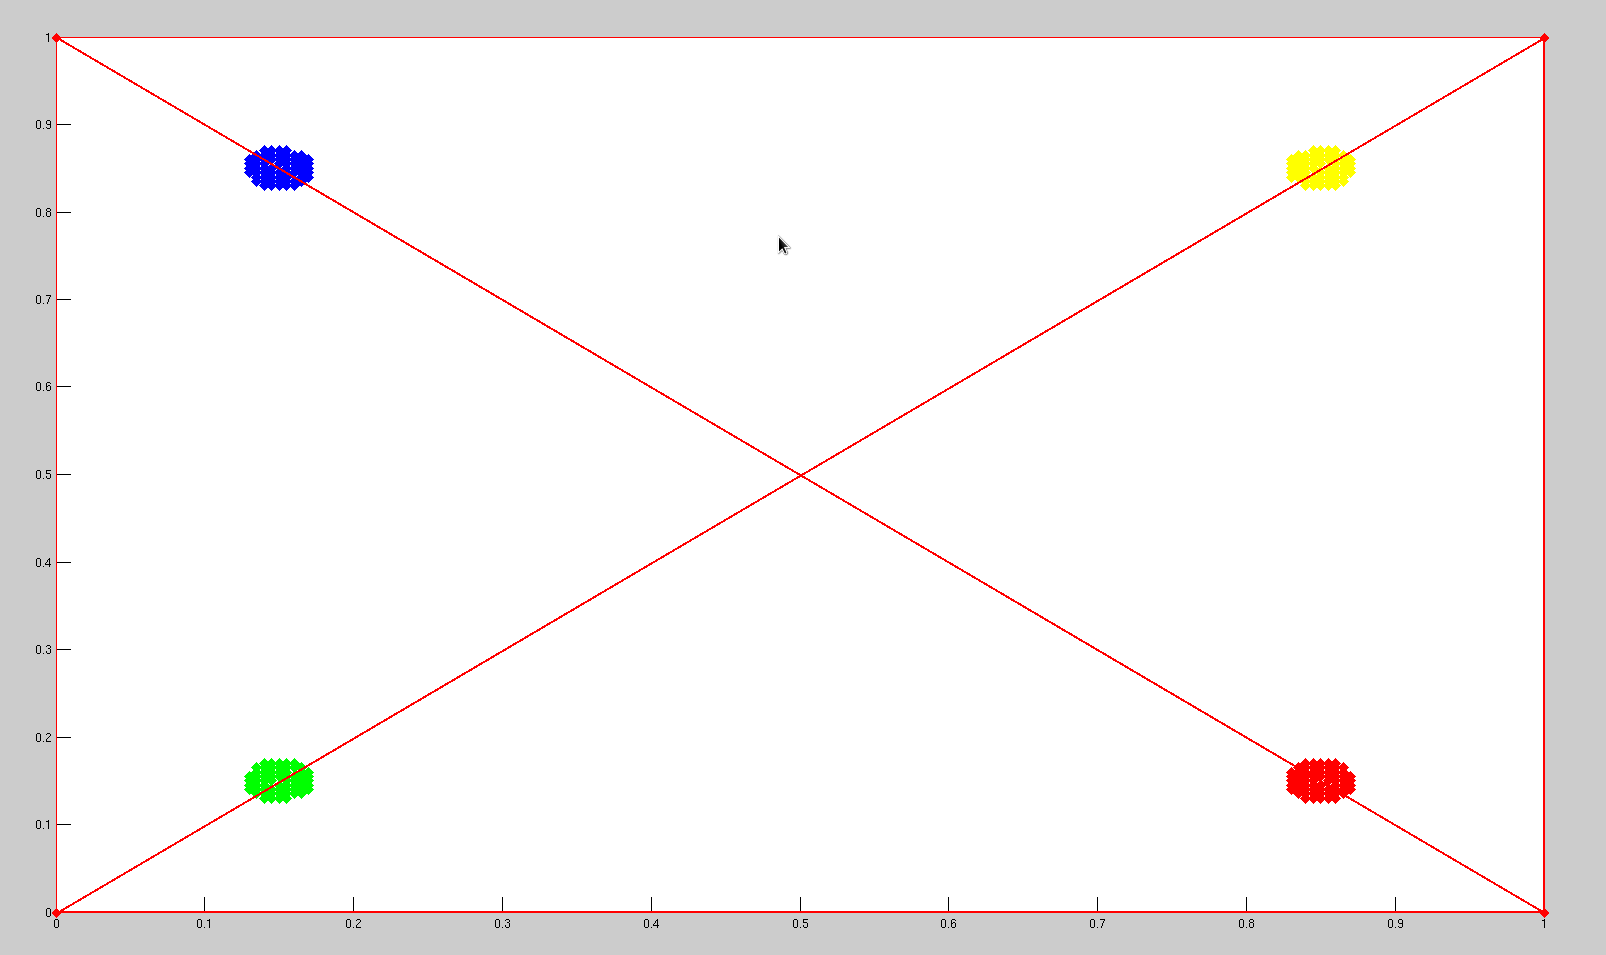
\includegraphics[width=.45\linewidth]{./chapter03/figures/critstab04.png}} 
\hfill
    \subfloat[D\'ecoupage de l'espace de travail en 
fonction du crit\`ere de stabilit\'e avec $Z = 0.5$]{\label{chap03:fig4view1}
    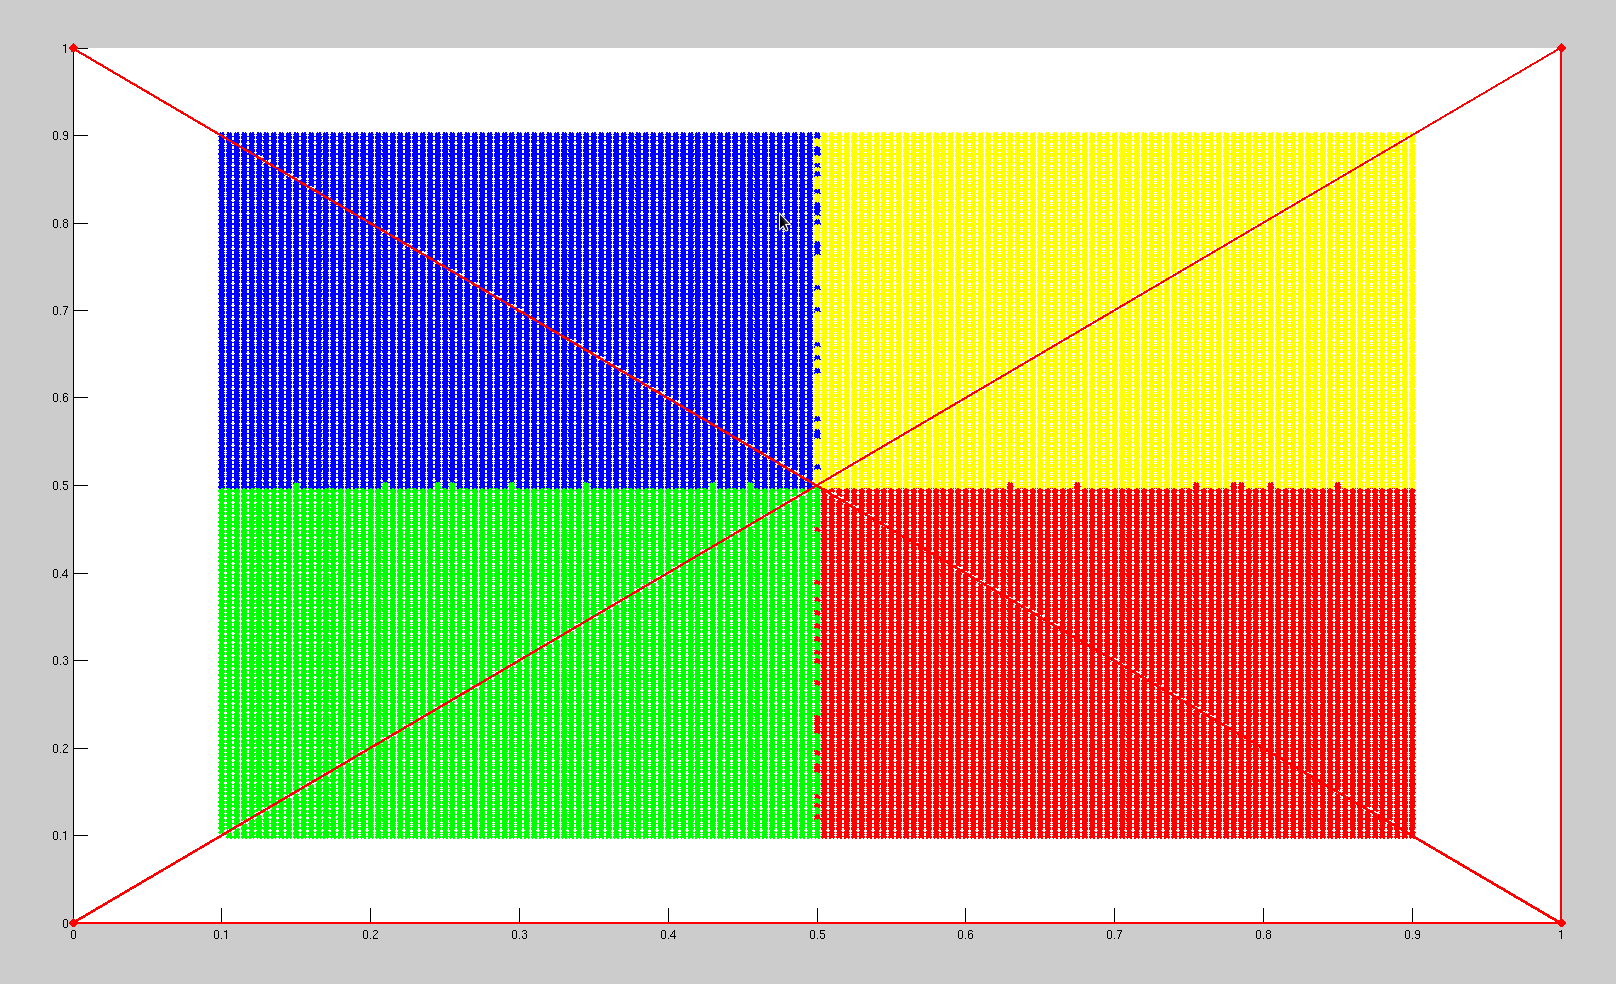
\includegraphics[width=.45\linewidth]{./chapter03/figures/critstab05.png}} 
\\
      \subfloat[Evolution du crit\`ere sur l'espace de 
travail avec $Z = 0.5$ (vue 3D)]{\label{chap03:fig4view2}
    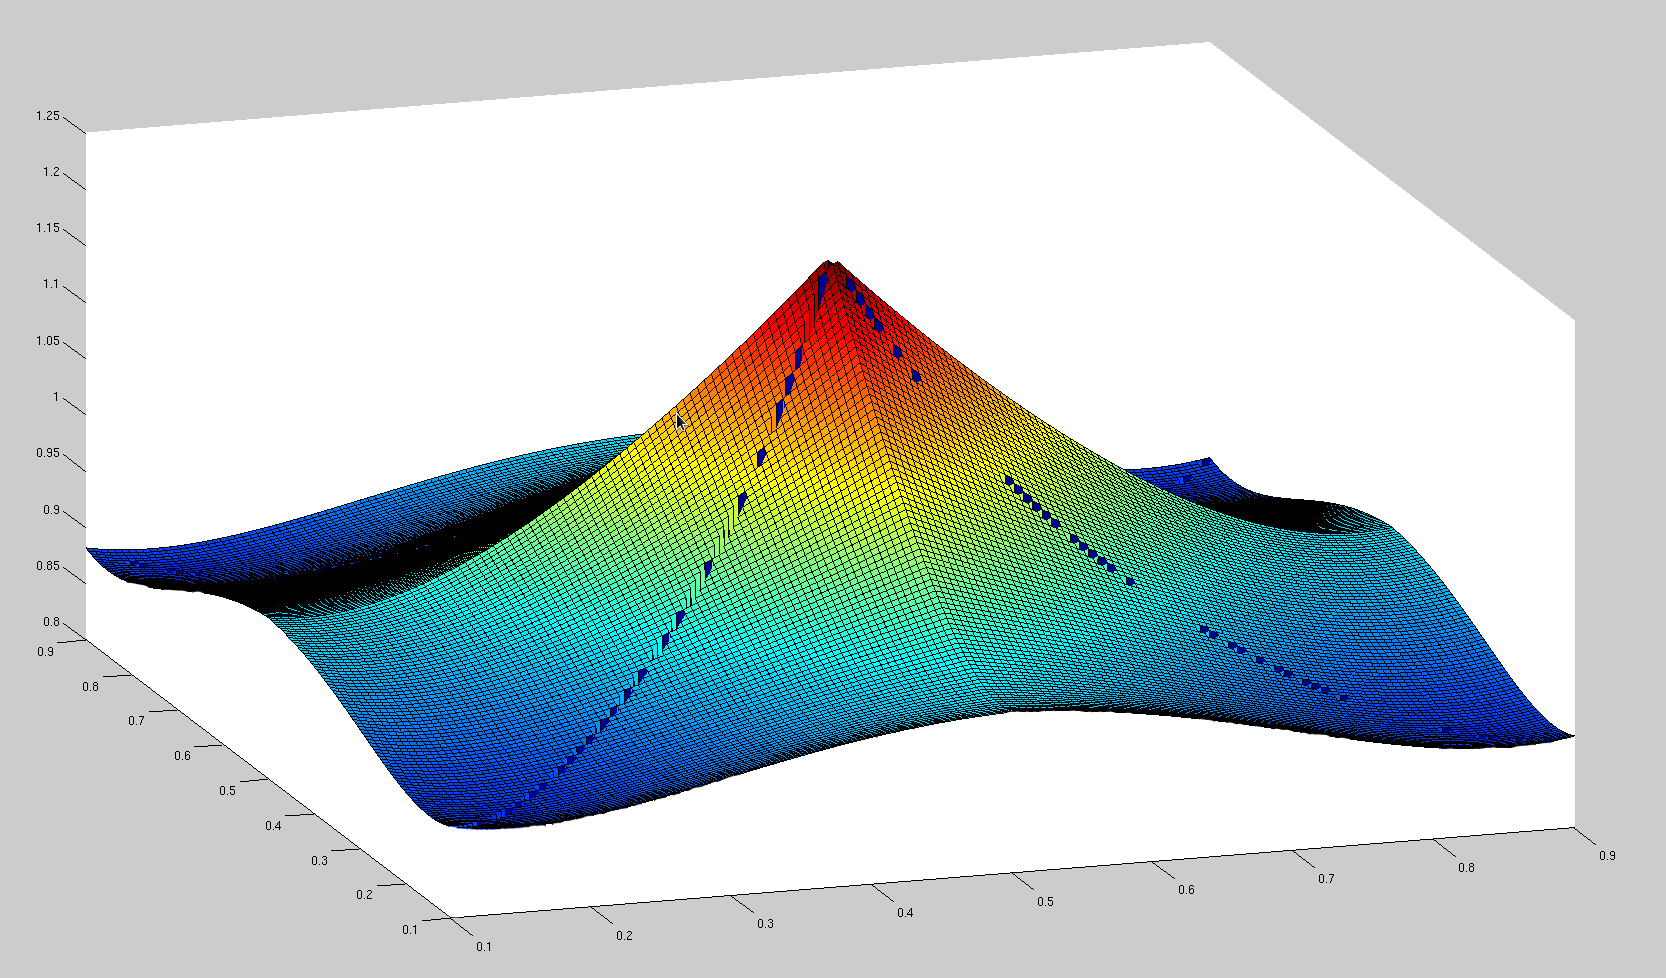
\includegraphics[width=.45\linewidth]{./chapter03/figures/critstab02.png}} 
\hfill
    \subfloat[Evolution du crit\`ere sur l'espace de 
travail avec $Z = 0.5$ (vue 2D)]{\label{chap03:fig4view3}
    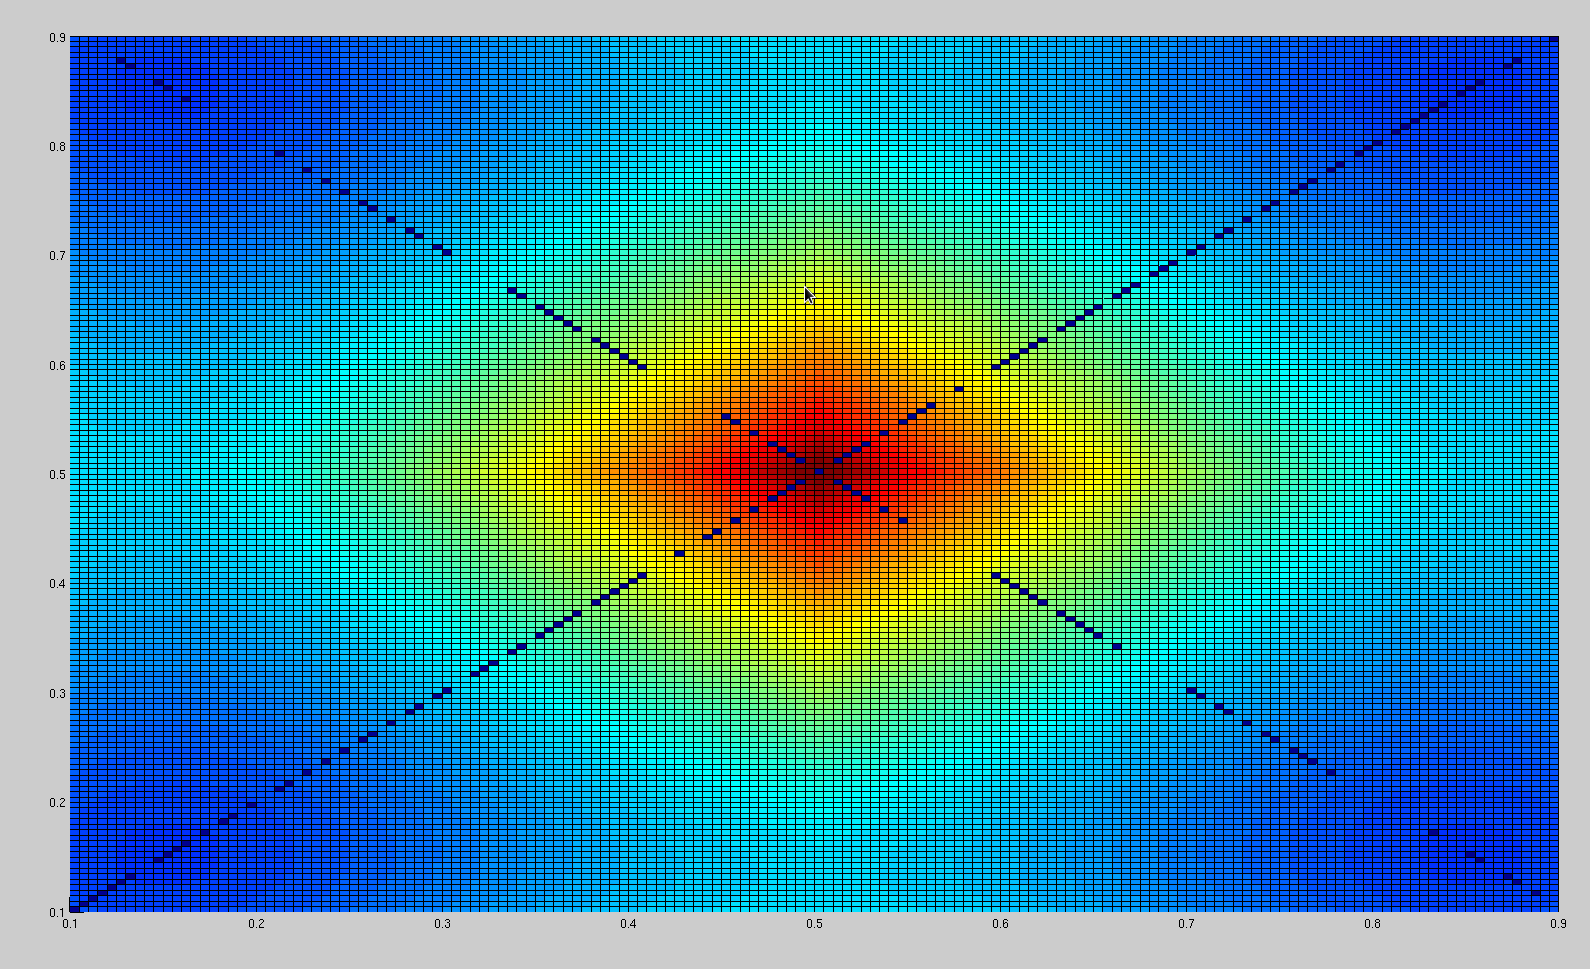
\includegraphics[width=.45\linewidth]{./chapter03/figures/critstab03.png}}
    \caption{\footnotesize Les deux figures en haut montrent comment (pour 
$Z = 0.5$) l'espace de travail est r\'eparti entre les sous-robots associ\'es 
aux configurations de c\^ables $\overline{CC}_i$: en rouge la configuration 
$\overline{CC}_{012}$, en vert la configuration $\overline{CC}_{013}$, en bleu 
la configuration $\overline{CC}_{023}$ et en jaune la configuration 
$\overline{CC}_{123}$. Les figures du bas montrent (toujours pour $Z = 0.5$) 
l'\'evolution du crit\`ere $\mathcal M_{\hbox{stab}}$ sur l'essentiel de 
l'espace de travail.}
\label{chap03:fig4}
\end{figure}

Les mesures respectives sont $\mathcal M_{\hbox {stab}_{013}} = 0.7822$ et 
$\mathcal M_{\hbox {stab}_{02}} = 0.9695$, soit une sélection de la 
configuration $\overline{CC}_{013}$.

Toutes ces mesures pouvant être réalisées en amont, elles n'impactent pas le 
temps de calcul de la commande. Ainsi, pour notre robot $4-1$ cubique, pour une 
valeur de $Z = 0.5$ fixée, les figures (\ref{chap03:fig4view0} et
\ref{chap03:fig4view1}) montrent quelle configuration de câbles sera 
privilégiée en tout point de l'espace de travail, et  les figures 
(\ref{chap03:fig4view2} et \ref{chap03:fig4view3}) l'évolution du critère sur 
l'ensemble de celui-ci.

\subsection{Am\'elioration de la pr\'ecision : minimiser l'influence des 
incertitudes articulaires}

La pr\'ecision actuelle du {\tt Marionet-Assist} sur lequel nous avons 
conduits nos exp\'erimentations n'exc\`ede pas $0.10m$ pour 
un espace de travail d'approximati\-vement $3mx3mx4m$. Nous avons en effet 
entrepris de placer le manipulateur dans une pose pr\'ealablement d\'ecid\'ee, 
puis ex\'ecut\'e deux aller-retours en mesurant les \'ecarts avec la position 
initiale une fois les retours accomplis. Les r\'esultats -- que l'on peut lire 
dans le tableau (\ref{chap03:tab01}) -- montrent que l'on atteint rapidement 
une 
erreur dont la norme $L^2$ est de $0.048m$. Rapport\'e \`a la taille de 
l'espace de travail, une telle pr\'ecision est plut\^ot performante, et 
satisfait les exigences requises pour l'usage originel du manipulateur. 
Toutefois, d\`es lors que nous avons entrepris d'ajouter des fonctionnalit\'es 
de manipulation d'objets du quotidien, la pr\'ecision requise doit \^etre 
inf\'erieure \`a $0.01m$. Nous verrons dans le chapitre suivant que 
l'asservissement visuel permet une telle am\'elioration des performances du 
robot, mais \'egalement que la qualit\'e de l'asservissement d\'epend de la 
configuration de c\^ables dans laquelle on se trouve. En effet, une incertitude 
sur les longueurs et leurs variations aura un effet sur la trajectoire et le 
positionnement. M\^eme si l'utilisation de l'asservissement en boucle 
ferm\'ee permettra de corriger ces erreurs, il est \'evidemment souhaitable de 
pouvoir les minimiser en amont, de mani\`ere \`a ce que l'utilisation de la 
vision permette des corrections mineures pour des trajectoires stables.  

\begin{table}[!h]
\begin{tabularx}{0.95\linewidth}{|p{0.15\linewidth}|X|X|X|}
\hline
& $X_1 $ & $X_2$ & $X_3$ \\
\hline
position(m) & (1.53,1.00,1.21) & (1.51,1.00,1.23) & (1.57,1.02,1.19)\\
\hline
error(m) & (0,0,0) & (-0.02,0.00,0.02) & (0.04,0.02,-0.02) \\
\hline
\end{tabularx}
\caption{La position ${\bf X}_1$ correspond \`a la position initiale, la 
position ${\bf X}_2$ \`a la position atteinte apr\`es un premier aller-retour 
(vers un point ${\bf Y} = (2.03,1.00,1.21)$), ${\bf X}_2$ la position apr\`es 
le second aller-retour.} 
\label{chap03:tab01}
\end{table}

Pour deux configurations de c\^ables donn\'ees, nous d\'efinissons la 
pr\'ecision associ\'ee comme l'erreur maximale sur la pose pour une incertitude 
sur les longueurs des c\^ables donn\'ee. Autrement dit, il s'agit de 
caract\'eriser l'influence des incertitudes articulaires sur les performances 
op\'erationnelles.

Pour cela, nous utilisons la relation suivante :
\begin{equation}
\Delta {\bf X} = {\bf J} \Delta {\bf \Theta}
\label{chap03:eq10}
\end{equation}

Entre deux configurations de c\^ables, nous souhaitons privil\'egier celle dont 
l'erreur maximale sur la pose en fonction de l'incertitude sur les longueurs de 
c\^ables sera inf\'erieure \`a toutes les autres.

Notre second crit\`ere devrait donc \^etre, avec $\delta {\bf \Theta}$ une 
incertitude maximale fix\'ee sur les coordonn\'ees articulaires :
\begin{equation}
\mathcal M_{\hbox{acc}} = ||{\bf J}  \delta {\bf \Theta} ||_{\infty}
\label{chap03:eq11}
\end{equation}
que nous chercherons \`a minimiser

Sinon reprenons l'exemple utilis\'e dans la section pr\'ec\'edente au point 
${\bf B} = (0.2,0.3,0.8)^T$, et que nous fixons $\delta \Theta$ \`a $0.10$m 
pour chacun des c\^ables\footnote{en pratique, la valeur de $\delta \Theta$ 
importe peu et peut-\^etre fix\'ee \`a un scalaire non-nul pr\`es 
puisque nous n'utilisons la relation que dans un objectif de comparaison.}, 
nous obtenons pour les configurations $\overline{CC}_{013}$ et 
$\overline{CC}_{023}$ respectivement :
$$\mathcal M_{\hbox{acc}_{013}} = ||(-0.0465, -0.0343, -0.3041)^T||_{\max} = 
0.3041$$ 
$$\mathcal M_{\hbox{acc}_{023}} = ||(-0.0327,-0.0343,-0.2902)^T||_{\max} = 
0.2902$$

L'erreur maximale est donc r\'ealis\'ee en profondeur, ce qui s'explique 
notamment par le fait que nous supposons les oppositions de forces se 
manifestent dans la jacobienne dans le plan, mais pas en profondeur car c'est la 
gravit\'e qui agit alors dans ce cas, et elle n'intervient pas dans la 
d\'efinition de la jacobienne.

D\`es lors, nous nous retrouvons ici avec un biais que nous corrigerons en ne 
consid\'erant que les erreurs de positionnement dans le plan, \'emettant donc 
l'hypoth\`ese que les erreurs sur la profondeur leur seront homog\`enes.

\begin{figure}[!htp]
  \centering
      \subfloat[R\'egions pour lesquelles le crit\`ere 
prend sa valeur minimale avec $Z = 0.5$ (256 points)]{\label{chap03:fig5view0}
    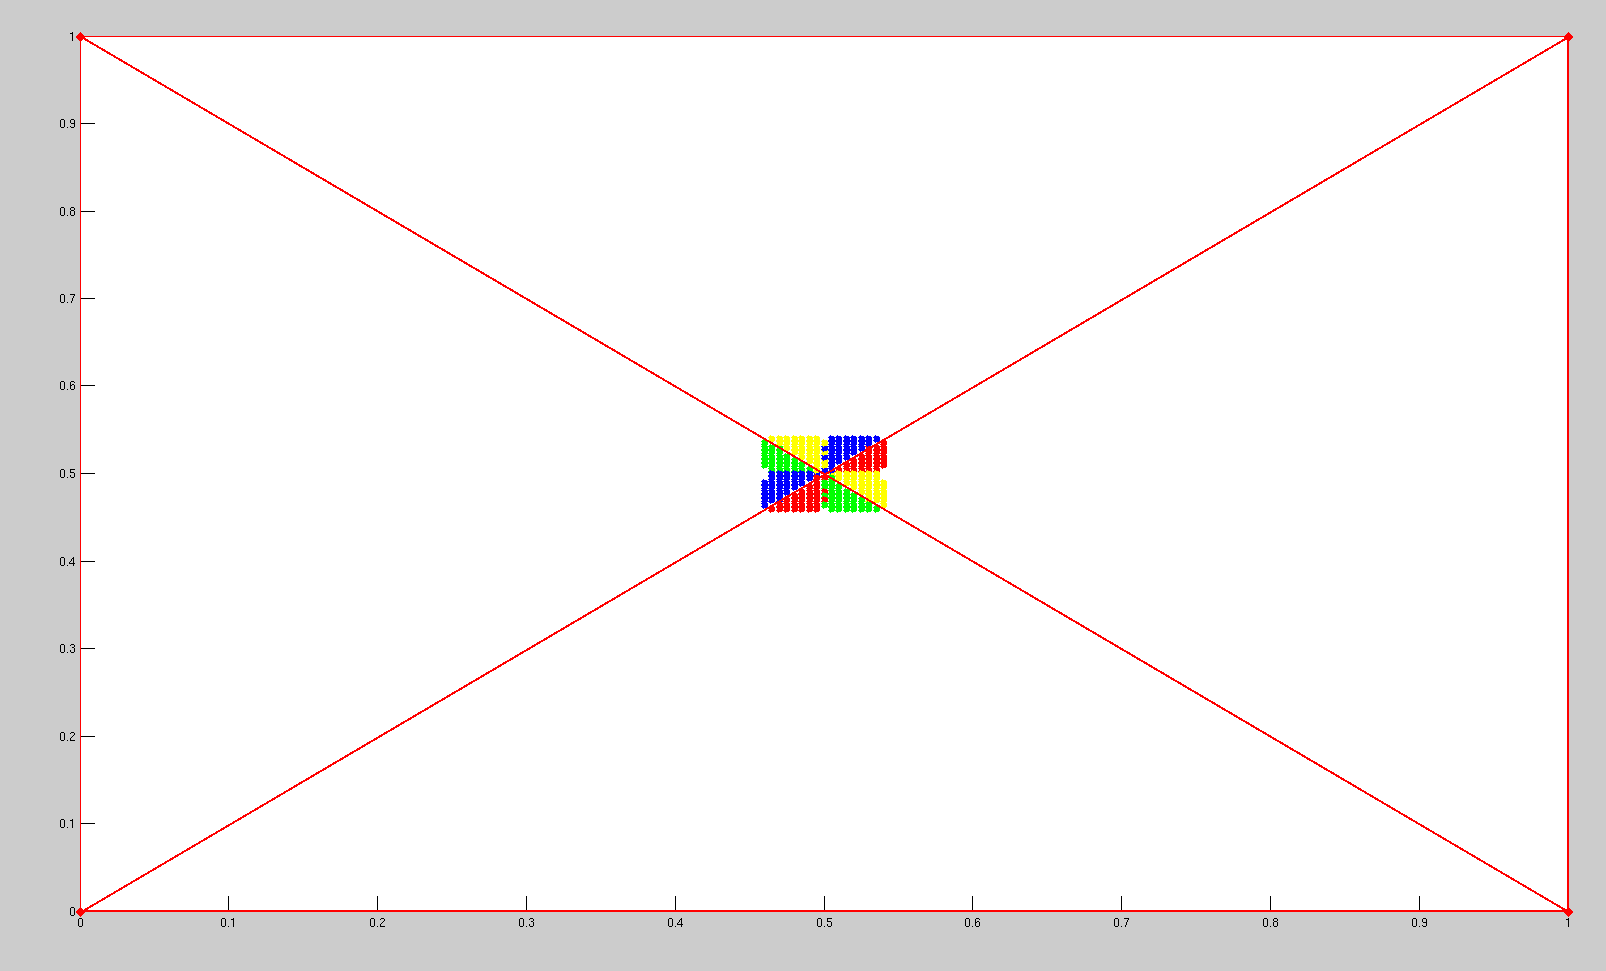
\includegraphics[width=.45\linewidth]{./chapter03/figures/crit_acc04.png}} 
\hfill
    \subfloat[D\'ecoupage de l'espace de travail en 
fonction du crit\`ere de pr\'ecision avec $Z = 0.5$]{\label{chap03:fig5view1}
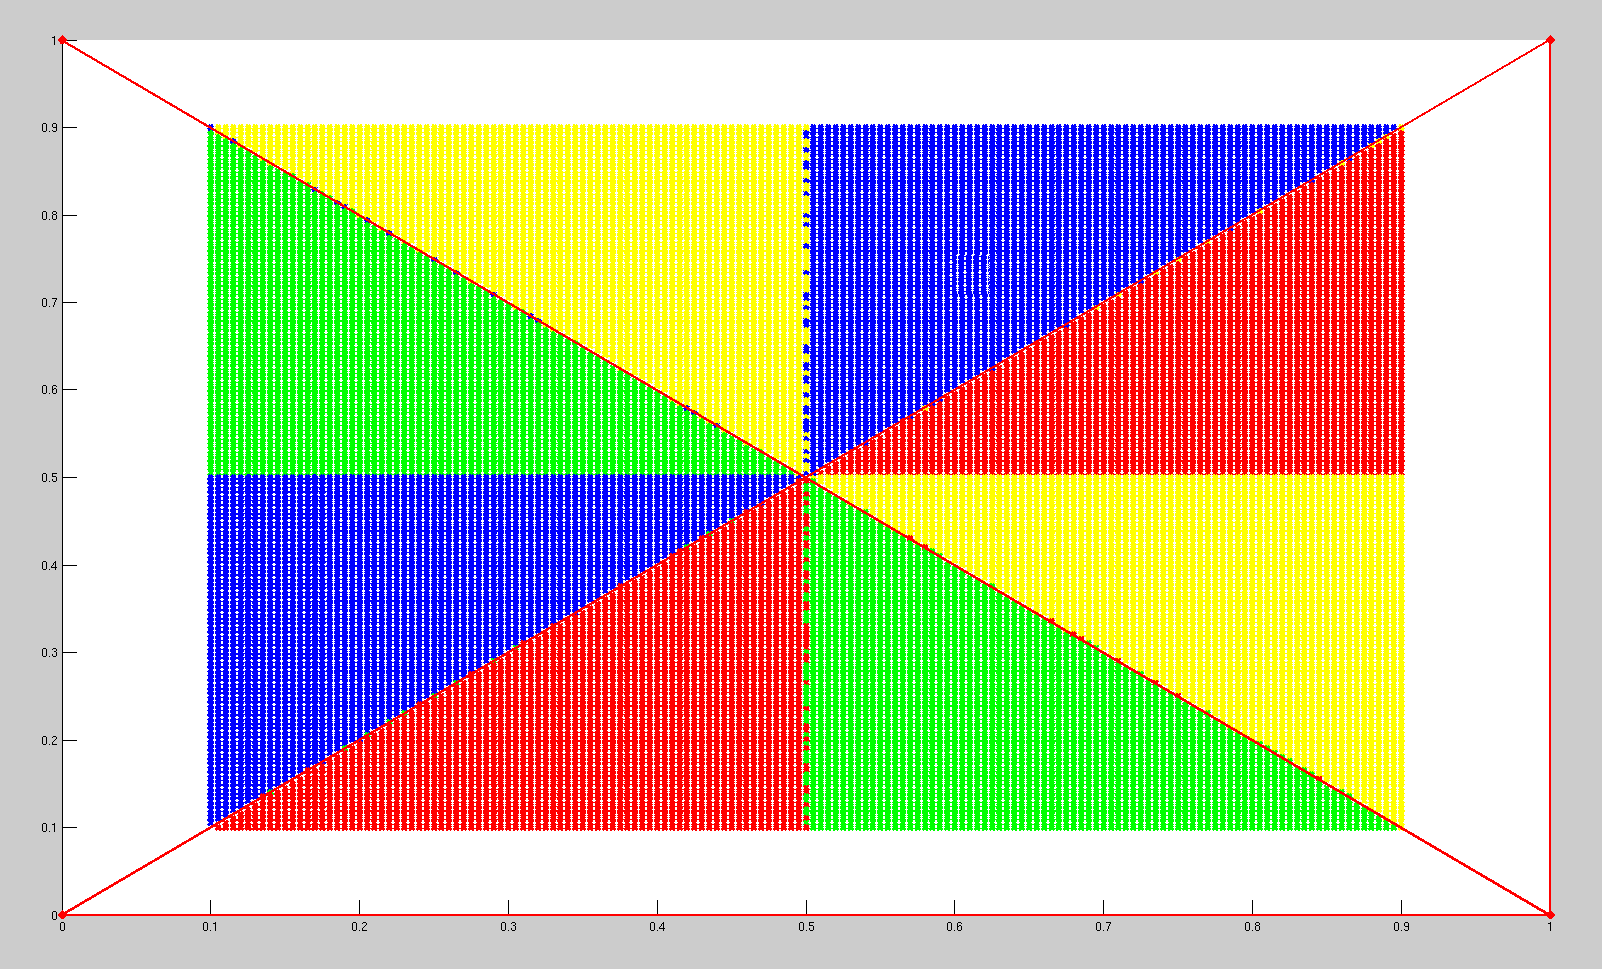
\includegraphics[width=.45\linewidth]{./chapter03/figures/crit_acc05.png}} \\
      \subfloat[Evolution du crit\`ere sur l'espace de 
travail avec $Z = 0.5$ (vue 3D)]{\label{chap03:fig5view2}
    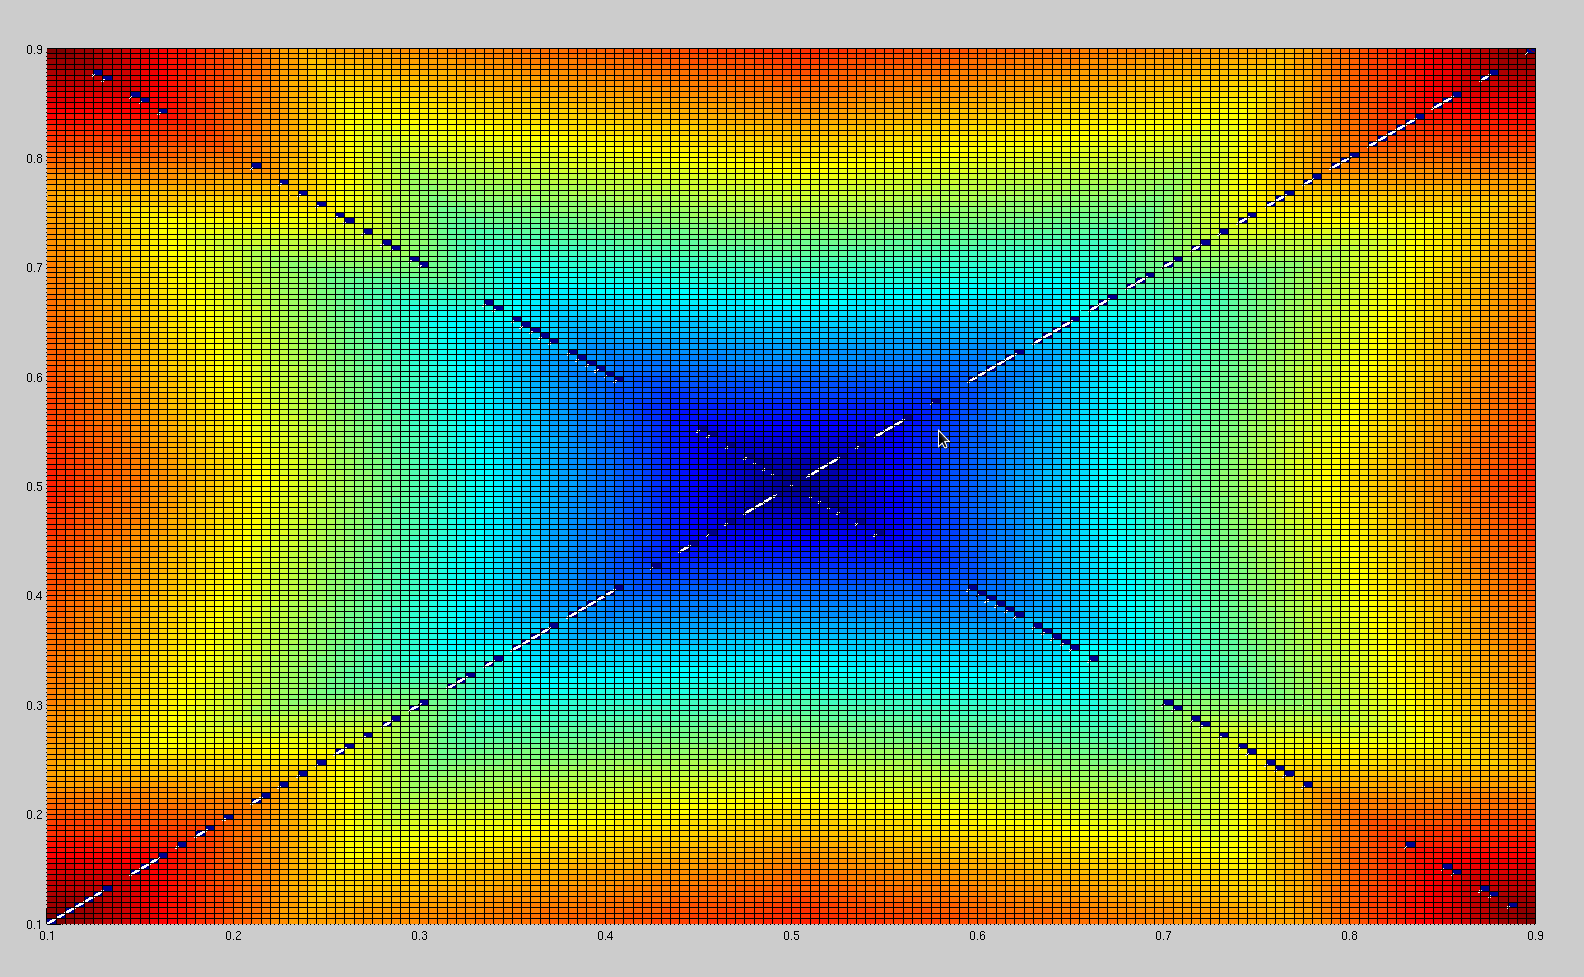
\includegraphics[width=.45\linewidth]{./chapter03/figures/crit_acc02.png}} 
\hfill
    \subfloat[Evolution du crit\`ere sur l'espace de 
travail avec $Z = 0.5$ (vue 2D)]{\label{chap03:fig5view3}
    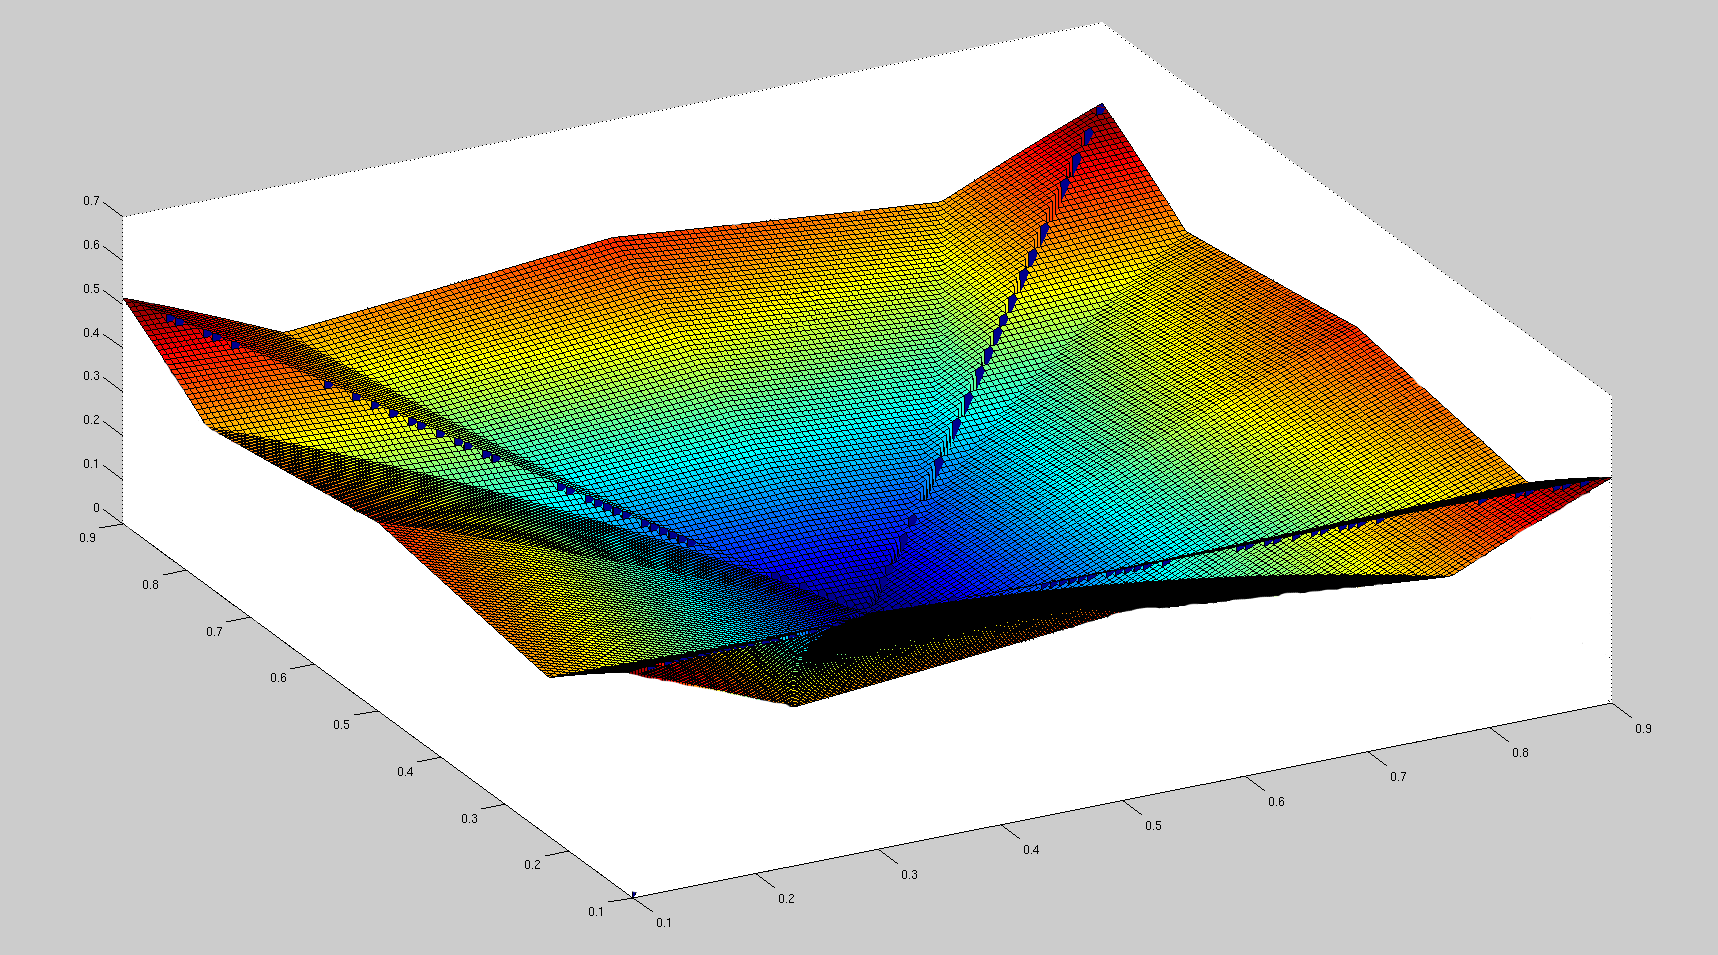
\includegraphics[width=.45\linewidth]{./chapter03/figures/crit_acc03.png}}
    \caption{\footnotesize Les deux figures en haut montrent comment (pour 
$Z = 0.5$) l'espace de travail est r\'eparti entre les sous-robots associ\'es 
aux configurations de c\^ables $\overline{CC}_i$: en rouge la configuration 
$\overline{CC}_{012}$, en vert la configuration $\overline{CC}_{013}$, en bleu 
la configuration $\overline{CC}_{023}$ et en jaune la configuration 
$\overline{CC}_{123}$. Les figures du bas montrent (toujours pour $Z = 0.5$) 
l'\'evolution du crit\`ere $\mathcal M_{\hbox{acc}}$ sur l'essentiel de 
l'espace de travail.}
\label{chap03:fig5}
\end{figure}

Le second crit\`ere est alors
\begin{equation}
\mathcal M_{\hbox{acc}} = \max_{x,y} |{\bf J} \delta {\bf \Theta}|
\label{chap03:eq11}
\end{equation}

Dans ce cadre, $\mathcal M_{\hbox{acc}_{013}} = 0.0465$ et 
$\mathcal M_{\hbox{acc}_{023}} = 0.0343$, ce qui revient \`a s\'electionner la 
configuration $\overline{CC}_{023}$ (ce qui \'etait d\'ej\`a le cas lorsque 
nous consid\'erions les erreurs sur la profondeur \`a partir de la relation 
\ref{chap03:eq10}).

Pour le point ${\bf B} = (0.3,.3,0.3)^T)$ dont les configurations de c\^ables 
possibles sont $\overline{CC}_{013}$ et $CC_{02}$, nous avons :
$$\mathcal M_{\hbox{acc}_{013}} = \max_{x,y} |(-0.0216,-0.0216,-0.1354)^T| = 
0.0216$$ 
$$\mathcal M_{\hbox{acc}_{02}} = \max_{x,y} |( -0.0197, -0.0197, -0.1338)^T| 
= 0.0197$$

Ici, la configuration $CC_{02}$ est pr\'ef\'er\'ee. Il s'agit toutefois d'un 
crit\`ere \'etabli pour une pose donn\'ee, alors que nous \'evoluons dans le 
cadre d'une trajectoire. Dans l'algorithme final qui sera pr\'esent\'e et 
illustr\'e en fin de chapitre, nous ajouterons une p\'enalit\'e \`a tout 
changement de configuration. Ainsi, si la trajectoire se d\'eroule dans notre 
cas int\'egralement dans le plan issu de la diagonale ${\bf A}_0{\bf A}_2$, il 
y aura du sens \`a rester dans certaines situations dans la configuration de 
c\^ables qui en est issue ; dans le cas contraire la p\'enalit\'e de transfert 
devrait conduire \`a basculer (ou rester) en configuration 
$\overline{CC}_{013}$.

Nous pouvons observer en (Fig.\ref{chap03:fig5}) la r\'epartition de l'espace 
de travail pour chaque sous-robot, ainsi que l'\'evolution du crit\`ere. 
Contrairement au crit\`ere de stabilit\'e, nous trouvons de nombreux transferts 
de type marginaux. Les figures (\ref{chap03:fig5view0} et 
\ref{chap03:fig5view1}) montrent en particulier que la pr\'ecision augmente 
d'autant plus que nous nous rapprochons du centre de l'espace de travail, ce qui 
n'\'etait pas le cas dans le cas de la recherche de stabilit\'e. Pour une 
incertitude de l'ordre de $0.10m$, nous avons mesur\'e sur l'espace de travail 
une moyenne d'incertitude de la pose \'egale \`a $0.0283m$ avec la s\'election 
de configurations de c\^ables, pour une moyenne de $0.0322m$ en nous basant sur 
le {\it pire des cas} (\`a savoir la plus mauvaise configuration de c\^ables en 
chaque point ; 1 chance sur 2 dans le cas du 4-1 qui poss\`ede en chaque pose 
deux configurations possibles).

\section{Certification de la m\'ethode}

Nous avons jusqu'ici consid\'er\'e que nous connaissions avec pr\'ecision la 
pose de l'organe terminal et donc des longueurs de c\^ables associ\'ees. En 
particulier, m\^eme lorsque nous avons observ\'e les influences des 
incertitudes sur les coordonn\'ees articulaires sur la pose, les 
valeurs des jacobiennes utilis\'ees (qui d\'epend \`a la fois de la pose et des 
longueurs de c\^ables) supposaient une exactitude parfaite des diff\'erentes 
coordonn\'ees. Dans le m\^eme temps, nous avons pu observer que cette 
hypoth\`ese n'\'etait pas tenable pour deux raisons :
\begin{itemize}
 \item la pose n'est connue qu'\`a une certaine impr\'ecision pr\`es, que nous 
pouvons certes am\'eliorer, mais qui implique n\'eanmoins que nous devions la 
prendre en compte dans l'ensemble des calculs
\item pr\`es des zones de transferts, une erreur de pose peut conduire \`a un 
changement de configuration de c\^ables ind\'esirable, et nous faire perdre 
donc 
les avantages gagn\'es jusqu'ici.
\end{itemize}

De plus, nous avons consid\'er\'e un robot id\'eal, dont nous connaissons 
parfaitement les points d'attaches formant un carr\'e parfait. Or, les robots 
parall\`eles \`a c\^ables et les {\tt Marionet} en particulier pr\'esentent 
l'avantage de pouvoir \^etre rapidement d\'eploy\'es du fait de la 
l\'eg\`eret\'e de l'\'equipement -- c'est le cas par exemple des robots con\c 
cus pour des interventions en situations de catastrophes naturelles -- et donc 
pouvoir s'adapter \`a leurs environnements. Nous devons en cons\'equence 
ajouter des incertitudes sur les points d'attache, sans quoi nous ne serions 
pas robustes aux variabilit\'es des environnements.

Afin de compl\'eter la m\'ethode, nous devons donc nous assurer que les 
r\'esultats sont valides malgr\'e les diff\'erentes incertitudes et 
impr\'ecisions. Il s'agit d\`es lors de {\it garantir} notre algorithme. Nous 
avons pour cela utilis\'e l'analyse par intervalles dont nous allons pr\'esenter 
les caract\'eristiques principales.

\subsection{L'analyse par intervalles}

L'analyse par intervalles a \'et\'e propos\'ee par \cite{moore1968} afin de 
prendre en compte les incertitudes dans les calculs. L'encadrement des variables 
et param\`etres permet de propager les incertitudes et d'obtenir ainsi 
des r\'esultats certifi\'es. L'analyse par intervalle a r\'ecemment \'et\'e 
utilis\'ee pour de l'\'etalonnage de robots \`a c\^ables \cite{sandretto2012}, 
pour le calcul de l'espace de travail de robots parall\`eles \`a c\^ables 
\cite{gouttefarde2011}, pour la r\'esolution du MGD des robots parall\`eles 
\cite{merlet2004solving} ou encore l'\'etalonnage de robots parall\`eles \`a 
l'aide de la vision \cite{daney2006interval}. Les algorithmes utilisant des 
intervalles pr\'esentent de plus l'avantage d'\^etre g\'en\'eralement 
parall\'elisables et donc d'exploiter pleinement les possibilit\'es du calcul 
distribu\'e.

On d\'efinit un intervalle $[x] = [\underline{x},\overline{x}]$ comme \'etant 
l'ensemble des r\'eels $x$ tels que $\underline{x} \leq x \leq \overline{x}$.
On utilisera les notations suivantes :
\begin{itemize}
 \item $\hbox{Min}([x]) = \underline{x}$
  \item $\hbox{Max}([x]) = \overline{x}$
  \item $\hbox{Mid}([x]) = (\overline{x} + \underline{x})/2$
   \item $\hbox{Diam}([x]) = \overline{x} + \underline{x}$
    \item $\hbox{Rad}([x]) = (\overline{x} + \underline{x})/2$
\end{itemize}

L'ensemble des intervalles \`a valeurs r\'eelles est not\'e $\mathbb I \mathbb 
R$.

Les op\'erations arithm\'etiques usuelles sont d\'efinies de la mani\`ere 
suivante :
\begin{itemize}
 \item addition : $[x]+[y] = [\underline{x},\overline{x}] + 
[\underline{y},\overline{y}] = [\underline{x} + 
\underline{y},\overline{x}+\overline{x}]$
\item soustraction : $[x]-[y] = [\underline{x},\overline{x}] - 
[\underline{y},\overline{y}] 
= [\underline{x} - \overline{y},\overline{x}-\underline{x}]$
\item multiplication : $[x]*[y] = [\underline{x},\overline{x}] * 
[\underline{y},\overline{y}] 
= [\min(\underline{x}\underline{y}, 
\underline{x}\overline{y},\overline{x}\underline{y},\overline{x}\overline{y}),
\max(\underline{x}\underline{y}, 
\underline{x}\overline{y},\overline{x}\underline{y},\overline{x}\overline{y})]$
\item division : if $0 \notin [y]$, $x/y = [\underline{x}, 
\overline{x}]*[1/\overline{y},1/\underline{y}]$ 
\end{itemize}

Un vecteur d'intervalles sera appel\'e une {\it bo\^ite} :
\begin{equation}
[x] \in \mathbb I \mathbb R^n, [x] = \begin{pmatrix}
                                      [x_1]\\
				      \dots \\
				      [x_n]
                                     \end{pmatrix}
\label{chap03:eq12}
\end{equation}

On dit de $[f]$ qu'elle est une {\it extension de $f$ aux intervalles} 
de la fonction $f$ si :
\begin{equation}
\begin{array}{ll}
\forall [x] \in \mathbb I \mathbb R, & \left \lbrace f(x), x \in [x] \right 
\rbrace \subseteq [f]([x]) \\
\forall x \in \mathbb R^n, & f(x) = [f](x) 
\end{array}
\label{chap03:eq13}
\end{equation}

Une extension aux intervalles conduit de mani\`ere g\'en\'erale \`a une 
surestimation de son co-domaine. Une telle surestimation sera not\'ee $\Box f = 
[f][x]$. Afin de diminuer cette surestimation, de nombreuses m\'ethodes ont 
\'et\'e d\'evelopp\'ees parmi lesquels les algorithmes de branchement et de 
contraction utilis\'es respectivement pour tester la pr\'esence de solutions 
dans un ensemble possible et r\'eduire la taille de cet ensemble possible.

Il est possible de red\'efinir toutes les fonctions \`a valeurs 
r\'eelles. En particulier, puisque nous souhaitons utiliser les intervalles 
sur l'\'equilibre statique (crit\`ere de stabilit\'e) et les \'equations de la 
cin\'ematique (crit\`ere de pr\'ecision), nous sommes int\'eress\'es par 
l'extension aux intervalles de la r\'esolutions des syst\`emes lin\'eaires 
\cite{hansen1980}.

Soit $[A]x = [b]$ un syst\`eme lin\'eaire dont les valeurs de $[A]$ et $[b]$ 
sont des intervalles. La solution prend la forme d'un intervalle $[x]$ pouvant 
\^etre de diff\'erentes natures selon le contexte dans lequel est pos\'e le 
syst\`eme :
\begin{itemize}
 \item $[x]_{\exists \exists} := \left \lbrace x ; \exists A \in [A], \exists b 
\in [b], Ax = b \right \rbrace$
 \item $[x]_{\exists \forall} := \left \lbrace x ; \exists A \in [A], \forall b 
\in [b], Ax = b \right \rbrace$
 \item $[x]_{\forall \forall} := \left \lbrace x ; \forall A \in [A], \forall b 
\in [b], Ax = b \right \rbrace$
 \item $[x]_{\forall \exists} := \left \lbrace x ; \forall A \in [A], \exists b 
\in [b], Ax = b \right \rbrace $
\end{itemize}

Afin de faire converger le plus possible la surestimation du domaine de 
r\'esolution $\Box x$ vers $[x]$, plusieurs m\'ethodes ont \'et\'e utilis\'ees 
dans le cadre de travail :
\begin{itemize}
 \item {\it Branch and Prune} (branchement)) : une premi\`ere bo\^ite globale 
$B_0$ est initialis\'ee sur l'ensemble de recherche. Cette bo\^ite est ensuite 
divis\'ee en plusieurs sous-bo\^ites. On teste la pr\'esence de solution dans 
chacune des sous-bo\^ites : si la solution n'y figure pas, la bo\^ite est 
rejet\'ee. Sinon, elle est \`a son tour divis\'ee en plusieurs bo\^ites sur 
lesquelles on testera la pr\'esence de solutions. L'algorithme est r\'ep\'et\'e 
jusqu'\`a ce que la taille des bo\^ites soit inf\'erieure \`a un certain seuil. 
On obtient ainsi un encadrement fin des solutions d'un syst\`eme.
  \item {\it redondance des variables} (contraction) : lorsqu'une m\^eme 
variable est utilis\'ee plusieurs fois, l'analyse par intervalle la consid\`ere 
cependant comme une variable ind\'ependante et surestime d\`es lors la 
propagation des incertitudes sur cette variable. Ainsi, pour $[x] = [-1,1]$, le 
calcul de $[x]*[x]$ donnera $[-1,1]$ alors que son co-domaine est $[0,1]$. 
Une analyse plus fine du syst\`eme prenant en compte la pr\'esence 
redondante d'une variable peut rapidement permettre de r\'eduire la taille 
de l'espace des solutions. Nous reviendrons d'ailleurs sp\'ecifiquement dans la 
section suivante sur deux utilisations particuli\`eres de la redondance des 
variables dans notre algorithme.  
\end{itemize}

En utilisant l'analyse par intervalles, nous assurons une robustesse aux 
erreurs et incertitudes, mais c'est au prix parfois d'une surestimation de 
leurs influences sur le mod\`ele et la commande. L'algorithme que nous allons 
exposer constitue l'\'equilibre que nous avons trouv\'e entre garantie maximale 
des r\'esultats et estimation la plus fid\`ele possible des espaces solutions.

\subsection{Algorithme utilisant l'analyse par intervalle}

Soit un robot $4-1$. Nous d\'efinissons les incertitudes suivantes : $\delta A$ 
repr\'esente l'incertitude sur la position des points de sortie des c\^ables, 
$\delta \rho$ d\'enote l'incertitude sur les longueurs de c\^ables et $\delta 
B$ correspond \`a l'incertitude sur la pose. Nous formons donc les intervalles 
suivants :
\begin{itemize}
 \item $[A_i] = [{\bf A}_i - \delta A/2,{\bf A}_i + \delta A/2]$ l'intervalle 
des localisations possibles du point de sortie du c\^able $i$
  \item $[\rho_i] = [\rho_i - \delta \rho /2,\rho_i + \delta \rho/2]$ 
l'intervalle des longueurs possibles pour le c\^able $i$
  \item $[B] = [{\bf B}_i - \delta B /2,{\bf B} + \delta B/2]$ l'intervalle 
des poses possibles de l'organe terminal.
\end{itemize}

Nous noterons de plus ${\bf \sharp B}$ la projection verticale de $\bf B$ sur 
le plan g\'en\'er\'e par les points ${\bf A_i}$ (suppos\'e horizontal). De la 
m\^eme mani\`ere, ${\bf \sharp A}_i$ correspondra en ces points aux seules 
coordonn\'ees dans le plan.

Une ligne de la jacobienne inverse correspondante devient :

\begin{equation}
[J^{-1}]_i = \left ( \frac {[B] - [A_i]}{[\rho_i]} \right )^T
\label{chap03:eq14}
\end{equation}

\subsubsection{D\'etermination des sites l\'egaux}

Soient $\mathcal O({\bf S}{\bf G})$ une s\'equence \`a r\'ealiser.

Dans un premier temps, nous cherchons \`a d\'eterminer les ensembles $Sl(S)$ et 
$Sl(G)$, \`a savoir l'ensemble des configurations de c\^ables possibles pour 
chacun de ces points, en prenant en compte les diff\'erentes incertitudes.

Dans le cas du robot $4-1$, trois situations sont possibles : \\

{\bf Configuration \`a 1 c\^able :}\\

Pour chaque c\^able, nous testons si $0 \in [\sharp B] - [\sharp A_i]$. Si 
c'est le cas, la configuration de c\^ables est conserv\'ee dans l'ensemble des 
configurations possibles.\\

{\bf Configuration \`a 2 c\^ables :}\\

Si ${\bf B}$ se trouve sur le segment de droite issu des points ${\bf 
\sharp A}_i$ et ${\bf \sharp A_j}$, alors il existe $\lambda \in ]0,1[$ tel que 
${\bf \sharp B} = {\bf \sharp A}_i + \lambda {\bf \sharp 
A}_i{\bf \sharp A}_j$.
L'extension de cette relation aux intervalles est alors :
\begin{equation}
\left \lbrace
\begin{matrix}
[B_x] = [A_{i_x}] + \lambda ([A_{j_x}] - [A_{i_x}]) \\
[B_y] = [A_{i_y}] + \lambda ([A_{j_y}] - [A_{i_y}])
\end{matrix}
\right .
\label{chap03:eq15}
\end{equation}

soit :

\begin{equation}
\left \lbrace
\begin{matrix}
\lambda_1 = \frac {[B_x] - [A_{i_x}]} {[A_{j_x}] - [A_{i_x}]}\\
\lambda_2 = \frac {[B_y] - [A_{i_y}]} {[A_{j_y}] - [A_{i_y}]}
\end{matrix}
\right .
\label{chap03:eq16}
\end{equation}

On peut remarquer que chaque ligne de l'\'equation est redondante concernant 
respectivement $[A_{i_x}]$ et $[A_{i_y}]$. Il est alors possible de 
r\'e\'ecrire le syst\`eme diff\'eremment, par exemple :
\begin{equation}
\left \lbrace
\begin{matrix}
\lambda_1 = \frac {[B_x] + [A_{j_x}]} {[A_{j_x}] - [A_{i_x}]} - 1\\
\lambda_2 = \frac {[B_y] + [A_{j_y}]} {[A_{j_y}] - [A_{i_y}]} - 1
\end{matrix}
\right .
\label{chap03:eq16}
\end{equation}
et de consid\'erer l'intersection des intervalles de solutions trouv\'ees.

Nous obtenons donc deux intervalles $[\lambda_1]$ et $[\lambda_2]$, dont nous 
allons prendre l'intersection $[\lambda] = [\lambda_1] \cap [\lambda_2]$. Nous 
testons ensuite si $0 < \overline{\lambda}$ et $\underline{\lambda} < 1$. Si 
c'est le cas, alors il existe dans notre intervalle une valeur pour laquelle le 
syst\`eme est v\'erif\'e ; potentiellement, ${\bf B} \in El(CC_{ij})$, et nous 
retenons la configuration. Dans le cas contraire, elle sera rejet\'ee.

Nous pouvons noter que dans le cas o\`u nous aurions $0 \in ([A_{j_x}] - 
[A_{i_x}])$ (ceci vaudra \'egalement pour $0 \in ([A_{j_y}] - [A_{i_y}])$), le 
test deviendra :
\begin{equation}
\begin{matrix}
\max(\overline{A_{i_x}},\overline{A_{j_x}}) > \overline{[B_x]},\\
\min(\underline{A_{i_x}},\underline{A_{j_x}}) < \underline{[B_x]}
\end{matrix}
\label{chap03:eq17}
\end{equation}
afin de nous assurer que ${\bf \sharp B}$ est potentiellement sur le segment 
${\bf \sharp A}_i{\bf \sharp A}_j$ mais bien dans les strictes limites de 
l'espace de travail.\\

{\bf Configuration \`a 3 c\^ables :}\\

Dans ce cas, nous devons v\'erifier que le point $\bf \sharp B$ se situe bien 
dans le triangle issu des points ${\bf \sharp A}_i$, ${\bf \sharp A}_j$ et 
${\bf \sharp A}_k$.

La relation que nous utilisons est la suivante : si $\bf \sharp B \in 
\widehat{{\bf \sharp A}_i{\bf \sharp A}_j{\bf \sharp A}_k}$, alors nous avons 
$(\lambda, \mu)$ tels que $0 < \lambda$, $0 < \mu$ et $\lambda + \mu < 1$ et :
\begin{equation}
{\bf A}_i {\bf B} = {\bf A}_i + \lambda {\bf A}_i{\bf A}_j + \mu {\bf A}_i{\bf 
A}_k  
\label{chap03:eq17}
\end{equation}
(\`a l'inversion pr\`es du r\^ole jou\'e par les points, ce que nous 
utiliserons entre autre pour contourner la redondance des variables dans 
l'\'equation).

Nous d\'eclinons cette relation pour chacune des coordonn\'ees, et nous 
obtenons ainsi le syst\`eme suivant :

\begin{equation}
\begin{bmatrix}
{\bf B}_{x} - {\bf A}_{i_x} \\
{\bf B}_{y} - {\bf A}_{i_y}
\end{bmatrix} =
\begin{bmatrix}
({\bf A}_{j_x} - {\bf A}_{i_x}) & ({\bf A}_{k_x} - {\bf A}_{i_x}) \\
({\bf A}_{j_y} - {\bf A}_{i_y}) & ({\bf A}_{k_y} - {\bf A}_{i_y})
\end{bmatrix}
\begin{bmatrix}
\lambda \\
\mu
\end{bmatrix}
\label{chap03:eq18}
\end{equation}

Un premier test \`a op\'erer est le calcul du d\'eterminant de la matrice du 
syst\`eme. Pour cela, nous faisons une \'evaluation par intervalles : si $0 \in 
[\hbox{Det}A]$, alors nous intervertissons les r\^oles jou\'es par les points, 
et si la situation se reproduit, alors nous rejetons la configuration.

Dans le cas d'un d\'eterminant non-nul, nous inversons le syst\`eme :

\begin{equation}
\begin{bmatrix}
\lambda \\
\mu
\end{bmatrix} = \frac 1 {\hbox{Det A}}
\begin{bmatrix}
({\bf A}_{k_y} - {\bf A}_{i_y}) & -({\bf A}_{k_x} 
- {\bf A}_{i_x}) \\
-({\bf A}_{j_y} - {\bf A}_{i_y}) & ({\bf A}_{j_x} - {\bf A}_{i_x}) 
\end{bmatrix}
\begin{bmatrix}
{\bf B}_{x} - {\bf A}_{i_x} \\
{\bf B}_{y} - {\bf A}_{i_y}
\end{bmatrix}
\label{chap03:eq19}
\end{equation}

Nous obtenons alors $[\lambda, \mu]$ sur lesquelles nous op\'erons deux types 
de tests :
\begin{itemize}
 \item si $0 < \underline{\lambda}, \underline{\mu}$ et $\overline{\lambda} + 
\overline{\mu} < 1$, alors $\bf B$ appartient avec certitude \`a l'espace 
l\'egal de la configuration de c\^ables test\'ee.
 \item si $0 < \overline{\lambda}, \overline{\mu}$ et $\underline{\lambda} + 
\underline{\mu} < 1$, alors il existe des couples $(\lambda, \mu) \in 
[\lambda]\times[\mu]$ qui v\'erifient les conditions d'appartenance. D\`es 
lors, nous ne pouvons exclure la possibilit\'e que le robot puisse utiliser la 
configuration de c\^ables test\'ee en cette pose aux incertitudes pr\`es. La 
configuration de c\^ables est donc conserv\'ee.
\end{itemize}

\begin{figure}[!htp]
  \centering
 \subfloat[Cas 01 : $\forall x \in \hbox{[}X\hbox{]},  F(x) \in 
I$]{\label{chap03:fig06view0}
 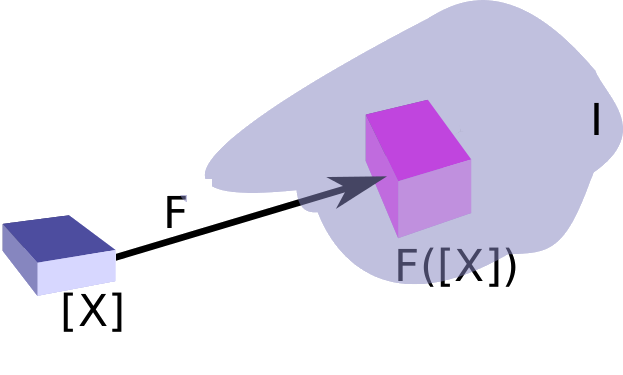
\includegraphics[width=.33\linewidth]{./chapter03/figures/interval_in.png}} 
\hfill
 \subfloat[Cas 02 : $\exists (x,y) \in \hbox{[}X\hbox{]}^2,  
F(x) 
\in I,  F(y) \notin I$]{\label{chap03:fig06view1}
 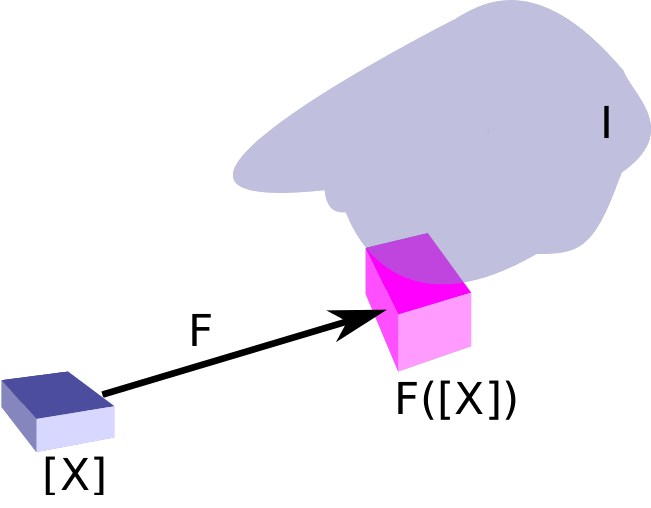
\includegraphics[width=.33\linewidth]{./chapter03/figures/interval_inout.png}} 
\hfill
  \subfloat[Cas 03 : $\forall x \in \hbox{[}X\hbox{]},F(x) 
\notin I$] 
{\label{chap03:fig06view2}
 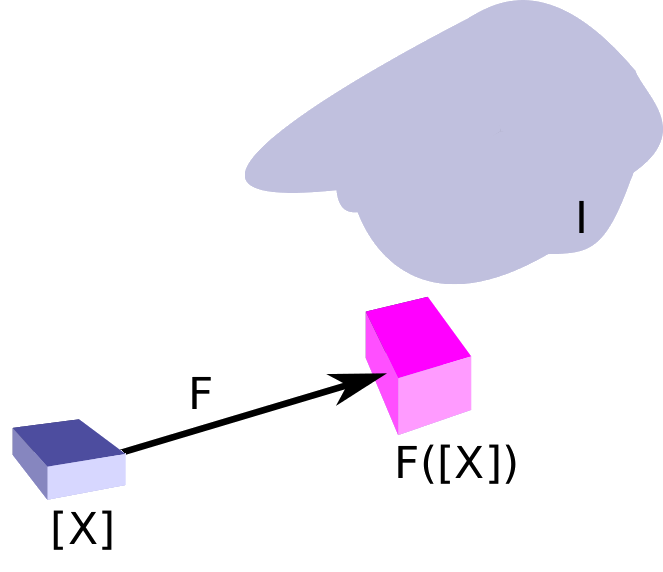
\includegraphics[width=.33\linewidth]{./chapter03/figures/interval_out.png}}
    \caption{\footnotesize{Trois situations de test d'appartenance : dans les 
cas $a$ et $b$, l'image par $[f]$ de $[x]$ permet de d\'ecider en toute 
certitude ; le cas $c$ ne permet pas de conclure : aux incertitudes s'ajoutent 
la surestimation \'eventuelle de l'image de $[X]$}}
\label{chap03:fig06}
\end{figure}

Nous nous trouvons \`a la fin de cette \'etape avec $3$ types de situations : 
des configurations de c\^ables possibles sous-contraintes, des configurations 
de $3$ c\^ables possibles, et des configurations de $3$ c\^ables certaines.

Nous attribuons un score \`a chacune de ces situations, que nous notons 
$\mathcal M_{CC}$.

\subsubsection{Mesure des crit\`eres}

{\bf Stabilit\'e :}\\

La relation utilis\'ee est ${\bf \tau} = {\bf J}^{T} {\boldmath \mathcal F}$. 
Nous consid\'erons ${\boldmath \mathcal F}$ comme un intervalle 
d\'eg\'en\'er\'e ($\underline{x} = \overline{x}$), et utilisons la jacobienne 
inverse \'etendue aux intervalles. Dans le cas des configurations de $3$ 
c\^ables, la formule d'inversion est connue et nous utilisons la redondance des 
variables pour contracter le vecteur d'intervalles solution pour les tensions. 
Le score calcul\'e pour une configuration de c\^ables est alors :

\begin{equation}
\mathcal M_{\hbox{stab}} = \sqrt{\sum_i \overline{\tau_i}^2}
\label{chap03:eq20}
\end{equation}\\

\noindent {\bf Pr\'ecision :}\\

Nous utilisons pour $\Delta \Theta$ la bo\^ite $[-\delta \rho/2, \delta 
\rho/2]^3$ ainsi que la jacobienne inverse \'etendue aux intervalles. Le 
r\'esultat obtenu est une bo\^ite $[\Delta X]$, \`a partir de laquelle nous 
d\'eduisons le score :

\begin{equation}
\mathcal M_{\hbox{acc}} = \max_{x,y}{\hbox{Abs}([|Delta X])}
\label{chap03:eq21}
\end{equation}
o\`u $\hbox{Abs}([X])$ est la fonction {\it valeur absolue} \'etendue aux 
intervalles.

\subsubsection{Hi\'erarchisation des s\'equences}

{\bf Optimisation globale :}\\

Nous n'avons consid\'er\'e ici que les s\'equences en ligne droite. Partant de 
${\bf S}$, nous recherchons l'ensemble des points ${\bf M}_i$ interm\'ediaires 
constituant la trajectoire aboutissant \`a $\bf G$. Si l'ensemble de la 
trajectoire ne peut \^etre r\'ealis\'ee avec une unique configuration de 
c\^ables, nous cherchons le meilleur point ${\bf M}_i$ pour r\'ealiser le 
transfert (ce point est unique dans le cadre d'un transfert marginal), et nous 
r\'eit\'erons l'op\'eration jusqu'\`a la r\'ealisation de la trajectoire. 
Plusieurs trajets sont alors obtenus, dont les scores respectifs sont :
\begin{equation}
\mathcal M_{\hbox{traj}} = \left (\sum_{i=1}^p \alpha \mathcal M_{CC_i} + \beta 
\mathcal M_{\hbox{stab}_i} + \gamma M_{\hbox{acc}_i} \right ) + \sum_{j = 
0}^{p-1} \mathcal M_{\hbox{trans}_j} 
\label{chap03:eq22}
\end{equation}
avec $\mathcal M_{\hbox{trans}_j}$ le score du transfert entre deux 
configurations de c\^ables donn\'ees, et $\alpha, \beta, \gamma$ des poids 
pond\'erant l'influence des diff\'erents crit\`eres.\\

\noindent {\bf Optimisation locale :}\\

Chaque point de la trajectoire est consid\'er\'e ind\'ependemment des autres ; 
on cherche alors \`a minimiser les crit\`eres s\'el\'ectionn\'es localement, ce 
qui peut aboutir \`a plus de changements de configurations (contr\^ol\'es par 
l'ajout artificiel de longueurs suppl\'ementaires pour les c\^ables que nous 
souhaitons disqualifier), mais \`a la s\'election de la configuration optimale 
\`a chaque moment. Il n'y a plus d\`es lors de calcul pr\'ealable du trajet, 
mais une adaptation \`a chaque instant de la trajectoire. Cette approche est 
particuli\`erement adapt\'ee aux asservissements en boucle ferm\'ee dont la 
trajectoire \'evolue en fonction des mesures effectu\'ees \`a chaque 
it\'eration. 

\section{Conclusions}

Lors de nos premi\`eres exp\'erimentations utilisant l'asservissement visuel 
pour des robots parall\`eles \`a c\^ables, nous avons rapidement r\'ealis\'e 
que les changements de configurations de c\^ables en affectait la qualit\'e, 
parfois jusqu'\`a en compromettre la r\'eussite lorsque les perturbations 
g\'en\'er\'ees par les changements nous faisaient perdre la cible dans l'image.

Nous avons d\`es lors entrepris de construire une strat\'egie nous permettant 
de choisir une configuration de c\^ables parmi toutes celles possibles en une 
pose donn\'ee, puis de d\'efinir des crit\`eres de comparaisons entre chacune 
d'entre-elles.

Dans ce but, nous avons commenc\'e par \'elaborer un formalisme propre aux 
configurations de c\^ables. Nous avons ensuite d\'efini une m\'ethode de 
d\'etermination des propri\'et\'es d'un syst\`eme en favorisant une approche 
{\it bottom-up} : le robot dit {\it maximal} est construit comme un syst\`eme 
collaboratif de plusieurs unit\'es pouvant se relayer une t\^ache dans des
conditions d\'etermin\'ees. Nous avons alors propos\'e des crit\`eres 
autorisant la hi\'erarchisation des trajets, compos\'es de trajectoires et de 
transferts.

Toutefois, afin d'assurer la robustesse de notre d\'emarche aux incertitudes, 
nous avons compl\'et\'e l'approche par l'utilisation de l'analyse par 
intervalles. Nous enfin enfin pr\'esent\'e les grandes lignes de l'algorithme 
final. Les simulations et exp\'erimentations seront pr\'esent\'ees dans le 
dernier chapitre de cette \'etude.

%\pagebreak

%% EXPES
%\include{validations/validations}

%\pagebreak

%% CONCLU
%\include{conclusions/conclusions}

\bibliographystyle{plain}
\bibliography{./biblio/bibliography}
\end{document}

Pour un triplet de c\^ables en tension, il est facile de montrer que 
l'\'equilibre statique est satisfait si le point ${\bf B}$ \`a sa projection 
dans le plan des ${\bf A}_i,{\bf A}_j,{\bf A}_k$ \`a l'int\'erieur du triangle 
constitu\'e par ces trois points. La figure (Fig.\ref{intro:fig11}) montre alors 
l'espace de travail atteignable pour chaque triplet de câbles en tension : on 
note qu'en tout point dont la projection verticale ne se trouve pas sur l'une 
des deux diagonales définies par les points $(A_0-A_2)$ et $(A_1-A_3)$, il 
existe pour chaque pose deux configurations possibles avec trois câbles en 
tension. Si la projection se trouve sur une diagonale, i lexiste une 
configuration qui a deux c\^ables en tension, \`a l'exception de l'intersection 
des diagonales pour laquelle nous avons deux configurations avec seulement deux 
c\^ables avec des $\tau > 0$.

\begin{figure}[!ht]
\centering
\def\svgwidth{.90\linewidth}
\input{./chapter0/figures/MA_corobots.pdf_tex}
\caption{\footnotesize{La figure au centre représente le robot {\tt 
Marionet-Assist} ; en bas à gauche est représenté l'espace de travail 
atteignable lorsque les câbles attachés aux points $A_0$, $A_1$, $A_3$ sont en 
tension, en bas à droite l'espace de travail atteignable pour les câbles reliés 
aux points $A_0$, $A_1$, $A_2$. En haut à gauche, nous avons l'espace de 
travail correspondant aux câbles $A_0$, $A_2$, $A_3$ en tension, et en haut à 
droite l'espace de travail atteignable pour les câbles attachés aux points 
$A_1$, $A_2$, $A_3$.}}
\label{intro:fig11}
\end{figure}



%%%%%%%%%%%%%%%%%%%%%%%%%%%%


en utilisant par exemple la g\'eom\'etrie pl\"uckerienne 
\cite{andreff:inria-00072393}, des descripteurs locaux ou globaux 
\cite{latuan2010}, ou encore des repr\'esentations fr\'equentielles (Fourier 
\cite{chari2008}, ondelettes \cite{ramosvelasco2012}). Le lecteur pourra 
retrouver les principales techniques dans \cite{marchand2005}.










%%%%%%%%%%%%%%%%%%%%%%%%%%%%%






Les manipulateurs parallèles à câbles peuvent s'avérer un choix pertinent 
d'architecture dès lors que tâche requiert tout ou partie des propriétés 
suivantes :
\begin{itemize}
 \item pouvoir être effectuée dans un large espace de travail
 \item pouvoir manipuler des charges importantes
 \item pouvoir être déployée rapidement
 \item garantir une précision et une dynamique suffisantes
\end{itemize}

Toutefois, nous avons vu que le contrôle de tels robots posait plusieurs 
problèmes, parmi lesquels :
\begin{itemize}
 \item des modèles géométriques et cinématiques plus complexes que pour les 
robots séries
  \item un câble ne pouvant exercer qu'une force unilatérale, il est 
possible qu'il se retrouve avec une tension nulle ; cela peut donner lieu à des 
changements discontinus des valeurs de tension pour chaque c\^able, voire la 
perte d'un ou plusieurs degrés de liberté
 \item des incertitudes mécaniques, particulièrement sur la longueur réelle de 
déploiement d'un c\^able si nous utilisons un moteur rotatif comme actionneur 
(le diamètre d'enroulement n'étant alors qu'une approximation).
\end{itemize}

Pour ces raisons, la précision d'une pose dépendra à la fois de son histoire 
(selon la trajectoire qui y a conduit et l'ensemble des câbles qui auront 
contribué à son obtention, le positionnement final pourra différer) et de sa 
robustesse aux incertitudes mécaniques, méthodologiques (simplification des 
modèles d'élasticité et de pesance des câbles par exemple) et de la précision 
des calculs.

L'asservissement visuel a donc été proposée à plusieurs reprises afin de 
résoudre tout ou partie de ces inconvénients. Les stratégies suivantes ont par 
exemple été mises en place :
\begin{itemize}
 \item une caméra déportée filme l'organe terminal, et par un asservissement en 
position, entreprend de corriger les erreurs de pose de celui-ci. Sont requis 
ici que la scène soit dégagée, que la caméra ait un champs de vision 
suffisamment grand pour pouvoir appréhender l'ensemble de l'espace de travail. 
Pour autant, une telle méthode ne permet pas de gérer les questions de tensions 
positives ou nulles dans les câbles.
 \item plusieurs caméras sont utilisées pour filmer les départs des câbles. En 
utilisant la géométrie plückerienne, ceci permet d'obtenir une estimation 
précise de la Jacobienne inverse. Pour autant, la question de la répartition 
des forces dans les câbles n'est là non plus pas considérée. Une telle 
stratégie suppose que tous les câbles soient en tension, ce qui est par exemple 
dans certaines architectures impossible, et peut donc conduire à une commande 
erronée. 
\end{itemize}

Pour autant, utilisées ensemble, ces deux stratégies devraient pouvoir 
permettre d'assurer la manipulation dans la plupart des cas, sans pour autant 
le garantir.

Notre objectif ici est donc double : construire dans un premier temps une loi 
de commande qui soit aussi indépendante que possible des paramètres de pose et 
des coordonnées articulaires, contrôler dans un deuxième temps les câbles qui 
seront en tension pour une trajectoire donnée. En effet, dès lors que nous 
connaissons les câbles qui sont en tension, nous obtenons le rang de la 
Jacobienne correspondante. Nous pouvons ainsi affiner la commande en cessant de 
considérer le robot global, pour ne plus prendre en compte que la partie 
correspondant réellement aux câbles qui agissent sur le déplacement. Nous 
utiliserons alors ce que nous définirons plus tard comme étant la {\it 
Jacobienne du sous-robot associe à une configuration de câbles}. L'utilisation 
d'une loi de commande articulaire exploitant des informations visuelles 
adaptées permettra de s'abstraire lors d'une commande cinématique à la fois des 
incertitudes liées à la commande du robot, mais également aux problèmes 
soulevés dans le chapitre précédent concernant l'estimation de la matrice 
d'interaction.

Ce chapitre est consacré à l'élaboration d'une telle loi de commande. Pour 
cela, nous présenterons dans un premier temps les spécificités d'un 
asservissement visuel classique de robots parallèles à câbles. Dans une seconde 
section, nous montrerons dans quelle mesure nous pouvons y trouver des 
améliorations concernant la précision du manipulateur et la robustesse aux 
erreurs et incertitudes diverses. La troisième section développera les 
conditions d'une loi de commande articulaire reposant sur une première 
estimation de la matrice d'interaction articulaire et un schéma itératif 
assurant la convergence vers une trajectoire linéaire. Enfin, une quatrième 
section présentera les conclusions de ce premier volet de notre étude. 
L'ensemble des simulations et validations expérimentales se trouveront dans le 
chapitre final.

\section{Elaboration d'un asservissement visuel des robots à c\^ables}

Cette première section est consacrée à l'élaboration d'une loi de commande 
classique adaptée aux robots parallèles à câbles. Ceci nous permettra de 
montrer les améliorations apportées par l'asservissement visuel (seconde section 
du chapitre) et servira de support de comparaison pour la loi simplifiée que 
nous proposerons en troisième section.

\subsection{Construction de la loi de commande classique}

Soit un robot parallèle à $m$ câbles contrôlant $n$ degrés de liberté. Pour 
rappel, la pose ${\bf X}$ de la plate-forme est la donnée des paramètres de 
pose donnant la position de la plate-forme dans l'espace ainsi que son 
orientation. Afin de commander la pose de la plate-forme, on contrôle les 
longueurs $\rho_i$ des câbles. Les câbles sont reliés au bâti en un point ${\bf 
A}_i$ que nous appelons {\it sortie de câble} et à l'organe terminal en un point 
${\bf B}_i$ que nous appelons {\it point d'attache}. En l'absence d'élasticité, 
de modèle de pesance, et en supposant une tension strictement positive, la 
longueur d'un câble sera égale à $||{\bf A}_i{\bf B}_i||$. Si la tension est 
nulle, sa longueur déroulée sera supérieure à la distance entre son point de 
sortie et son point d'attache.

Les équations de la cinématique inverse permettent de construire la relation 
suivante entre les variations de la pose de l'organe terminal ${\bf \dot X}$ et 
les variations des coordonnées articulaires ${\dot \brho}$ :
\begin{equation}
  \dot {\brho} = {\bf J}^{-1} {\bf \dot X} 
 \label{chap02:eq0}
\end{equation}

La matrice ${\bf J}^{-1}$ dépend tout autant de la pose de l'effecteur que des 
longueurs de câbles. Ses lignes sont données par :
\begin{equation}
  {\bf J}^{-1}_i = \begin{bmatrix}
                   \frac {{\bf A}_i {\bf B}_i} \rho & \frac {{\bf C}{\bf B}_i 
\times {\bf A}_i {\bf B}_i} \rho
                   \end{bmatrix}
 \label{chap02:eq1}
\end{equation}
${\bf C}$ étant un point de la plate-forme préalablement choisi.

Ainsi, un déplacement pratique s'éloigne nécessairement de la trajectoire 
théorique, la convergence étant assurée par un schéma itératif permettant de 
corriger la commande cinématique. L'erreur sera d'autant plus faible que la 
fréquence de la commande sera élevée, permettant des déplacements plus petits 
et donc un écart moins important.

A l'itération suivante, la Jacobienne est calculée à partir de la pose et des 
coordonnées articulaires théoriques, qui peuvent différer de la pose et des 
longueurs de câbles réelles. Dès lors, la dérive risque de se propager. Sans 
stratégie de relecture des variables articulaires ou d'estimation de la pose 
(par le biais en particulier de capteurs supplémentaires), un contrôle 
cinématique risque d'échouer sur une trajectoire suffisamment grande. Sa 
précision en tous les cas n'est pas garantie et deviendra problématique sur une 
trajectoire suffisamment longue.

Une manière alternative de corriger cette dérive consiste en l'utilisation de 
l'asservissement visuel. Si l'évolution de l'erreur entre les mesures 
effectuées dans l'image courante et les mesures désirées donne une indication 
du déplacement à effectuer pour converger vers l'objectif, elle reflète 
également les conséquences de la dérive du manipulateur et la correction sera 
alors intégrée à sa consigne.

La loi de commande finale est donn\'ee par la relation :
\begin{equation}
 \dot \brho = -\lambda {\bf J}^{-1}  {}^e \mathcal R_c \widehat {{\bf L}^*_e} 
{\bf e} \label{chap02:eq2}
\end{equation}
o\`u ${}^e \mathcal R_c$ d\'enote la matrice permettant de passer du 
r\'ef\'erentiel de la cam\'era au r\'ef\'erentiel de l'organe terminal.


\subsection{Utilisation des moments 2D}

\subsection{Cas du robot N-1}

\section{Amélioration de la robustesse et de la précision}

\subsection{Robustesse aux incertitudes de modèle}

\subsection{Amélioration de la précision}

\subsection{Illustration des limites avec le cas N-1}


\section{Asservissement simplifié : commande articulaire}

\subsection{Motivations}

\subsection{Le schéma de Broyden}

\subsection{Commande simplifiée}

\subsection{Cas N-1}

\section{Conclusions}